% Document For Use With LuaLaTeX
\documentclass[a4paper,11pt]{book}

% Define Thesis Information
\newcommand{\thesistitle}{On the Influence of Surface Effects of Electrically Biased Semiconductor Nanostructures in Off-Axis Electron Holography}
\newcommand{\thesisauthor}{Hüseyin Çelik}
\newcommand{\submissiondate}{1\textsuperscript{st} August 2023}

% Fonts and Typography
\usepackage[ngerman,english]{babel}
\usepackage{fontspec,microtype}

% Figures, Graphics and Captions
\usepackage[dvipsnames]{xcolor}
\usepackage{graphicx,caption,subcaption}

% Math and Science
\usepackage[locale=US,per-mode=fraction,separate-uncertainty,sticky-per,retain-explicit-plus]{siunitx}
\usepackage[tbtags]{mathtools}
\usepackage{amssymb,physics,interval}

% Bibliography
\usepackage[style=numeric-comp,sorting=none,giveninits=true,doi=false,isbn=false]{biblatex}
\usepackage[nottoc]{tocbibind}
\usepackage{csquotes}

% Style and Layout
\usepackage[all]{nowidow}
\usepackage[Sonny]{fncychap}
\usepackage{parskip,emptypage,fancyhdr}

% Patching LaTeX Packages
\usepackage{xpatch,ifthen}

% Links
\usepackage[hidelinks,pdfauthor={\thesisauthor},pdftitle={\thesistitle}]{hyperref}
\usepackage[nameinlink,noabbrev]{cleveref}

% Load After Hyperref
\usepackage[top=1in,bottom=1in,outer=1in,inner=1.5in]{geometry}
\usepackage{float,xurl,doi}

% Check Emptiness
\newcommand{\ifempty}[2]{
   \ifthenelse{\equal{#1}{}} {#2} {\protect\emph{\protect\nouppercase#1}}%
}

% Default Header and Footer
\pagestyle{fancy}
\fancyhf{}
\fancyhead[LE]{\emph{\nouppercase\leftmark}}
\fancyhead[RO]{\ifempty {\rightmark} {\emph{\nouppercase\leftmark}}}
\fancyfoot[LE,RO]{\thepage}
\renewcommand{\headrulewidth}{0pt}%
\renewcommand{\footrulewidth}{0pt}%
\setlength{\headheight}{14pt}

% Plain Header and Footer
\fancypagestyle{plain}{%
   \fancyhf{}
   \fancyfoot[LE,RO]{\thepage}
   \renewcommand{\headrulewidth}{0pt}
   \renewcommand{\footrulewidth}{0pt}
   \setlength{\headheight}{14pt}}

% Continue Footnote Numbering Across Chapters
\counterwithout{footnote}{chapter}

% Enable French Spacing
\frenchspacing

% Add Bibliography File
\addbibresource{References.bib}

% Caption Style
\captionsetup{labelfont={bf,sf}}

\begin{document}

\pagenumbering{Alph}
\begin{titlepage}
	\begin{figure}[H]
	\centering
	
\includegraphics[scale=2]{Figures/Logo.pdf}
	\end{figure}
	{\center
	{\LARGE
	\textbf{Faculty II}\\
	Institute of Optics and Atomic Physics}\\
	\vspace*{\fill}

	\hrulefill

	{\Huge \textbf{\thesistitle}\par}

	\hrulefill

	\vspace*{\fill}
	{\LARGE Master Thesis}\\
	\emph{submitted for the degree of Master of Science (M.\,Sc.)}\\
	\vspace*{\fill}
	by\\
	{\Large \textbf{\thesisauthor}}\\
	(Student-No. 0 390 823)\\
	}
	\vspace*{10mm}
	\begin{tabbing}
	\hspace*{4cm}First Examiner: \hspace*{1cm}\=Prof.~Dr.~Michael Lehmann\\
	\hspace*{4cm}Second Examiner: \>Dr.~Andrei Schliwa\\
	\hspace*{4cm}Supervisor: \>Dr.~Tolga Wagner\\
	\hspace*{4cm}Date of Submission: \>\submissiondate \\
	\end{tabbing}
\end{titlepage}


\frontmatter
\newgeometry{top=1in,bottom=1in,outer=1in,inner=1.5in,includeheadfoot}
\chapter*{Declaration of Originality}
I hereby declare that the thesis submitted is my own, unaided work, completed without any unpermitted external help. Only the sources and resources listed were used.

The independent and unaided completion of the thesis is affirmed by affidavit:

\vspace*{1cm}
\hspace*{3.2cm} \includegraphics[scale=0.2]{Figures/Signature.pdf}
\vspace*{-1cm}

\begin{tabular}{@{}p{2cm}p{8cm}@{}}
	\textbf{Signature:} & \hrulefill \\
	& \thesisauthor \\
	& Berlin, \submissiondate \\
\end{tabular}

\chapter*{Abstract}
The aim of the present thesis is to investigate the influence of surface effects of electrically biased semiconductor nanostructures on electron holographic measurements. A significant influence is played by the stray fields above and below the specimen, which in turn are defined by the electrostatic potential distribution within the specimen (especially in the propagation direction of the electron beam). However, a quantitative description of such ever-smaller devices has so far required tomographic approaches, which entail a significant measurement effort, or modeling by means of established simulation methods, which are highly computationally intensive and require knowledge of the microscopic charge carrier distribution.

These circumstances are addressed here by introducing a simple and intuitive model for the approximation of complex electrostatic potential distributions. The self-developed model uses only independent convolutions of an initial potential distribution with a (normalized) propagation distance dependent 1D~Gaussian kernel and thus allows the reconstruction of the entire electrostatic potential distribution of a real-world specimen from only one measured projection. This enables the approximation of the stray fields above and below as well as the electrostatic potential distribution within the specimen. Through the excellent agreement in comparison with tomographic measurements, the self-developed model was validated. Consequently, a significant reduction of the required computational power as well as a drastically simplified measurement process is enabled, opening up new possibilities for quantitative electron holographic investigations of semiconductor nanostructures.
\begin{otherlanguage}{ngerman}
\chapter*{Deutsche Zusammenfassung}
Ziel der vorliegenden Arbeit ist die Untersuchung des Einflusses von Oberflächeneffekten elektrisch geschalteter Halbleiternanostrukturen auf elektronenholographische Messungen. Einen signifikanten Einfluss spielen hierbei die Streufelder über- und unterhalb der Probe, welche wiederum durch die elektrostatische Potentialverteilung innerhalb der Probe (insbesondere in Ausbreitungsrichtung des Elektronenstrahls) bestimmt sind. Eine quantitative Beschreibung solcher immer kleiner werdenden Bauelemente erforderte jedoch bis jetzt tomographische Ansätze, welche einen signifikanten Messaufwand mit sich führen, oder die Modellierung mittels etablierten Simulationsmethoden, welche höchst rechenintensiv sind und eine Kenntnisse über die mikroskopische Ladungsträgerverteilung erfordern.

Diese Umstände werden hier durch die Einführung eines simplen und intuitiven Modells zur Approximation komplexer elektrostatischer Potentialverteilung angegangen. Das selbstentwickelte Modell verwendet nur unabhängige Faltungen einer anfänglichen Potentialverteilung mit einem (normalisierten) von der Ausbreitungsdistanz abhängigen 1D~Gaußschen Kernel und erlaubt so die Rekonstruktion der gesamten elektrostatischen Potentialverteilung einer realen Probe aus nur einer gemessenen Projektion. Hiermit lassen sich sowohl die Streufelder über- und unterhalb als auch die elektrostatische Potentialverteilung innerhalb der Probe approximieren. Durch die exzellente Übereinstimmung im Vergleich mit tomographischen Messungen konnte das selbstentwickelte Modell validiert werden. Dies ermöglicht eine signifikante Reduktion der benötigten Rechenleistung sowie eine drastische Vereinfachung des Messprozesses und eröffnet neue Möglichkeiten für quantitative elektronenholographische Untersuchungen von Halbleiternanostrukturen.
\end{otherlanguage}


\tableofcontents

\mainmatter
\chapter{Introduction} \label{chap:introduction}
With its continuous developments, the semiconductor industry plays a central role in today's technology-driven society \cite{More1965,Bank1990,Smith1997,Alferov1998,Flamm2003,Wachutka2004,Jenkins2005,Lukasiak2010,Mack2011,Klein2016,Leiserson2020}. In this context, the theoretical understanding of the underlying physical processes (e.\,g.\ from analytical models or numerical simulations) and investigation-based knowledge about their real-world behavior (e.\,g.\ from experimental observations) do not always go hand in hand, which is particularly evident in the course of the progressive miniaturization of semiconductor structures (e.\,g.\ semiconductor nanostructures) in order to increase their efficiency by means of power consumption \cite{Twitchett2002,Beleggia2003,Cooper2006,Cooper2007,Twitchett-Harrison2007,Cooper2009,Somodi2013,Yazdi2015}. A precise knowledge of the electrostatic potential distribution of these kind of real-world devices would open the door to a better understanding of their electrical properties. Perhaps the most established transmission electron microscopic (TEM) and thus imaging technique for the investigation of electrostatic potential distributions in semiconductor structures in the $\si{\nm}$~range is off-axis electron holography (EH) \cite{Lichte1986,Tonomura1987,Cowley1992,DuninBorkowski2004}. Combined with a tomographic approach, EH has demonstrated the increasing influence of TEM-specimens' surface effects (e.\,g.\ the broadening of depletion regions or preparation-related artifacts) with a continuous reduction of the structural dimensions \cite{Twitchett-Harrison2007,Miao2016}.

However, taking this approach to a quantitative level necessitates a comparison with conventional simulation methods (e.\,g.\ finite element method (FEM)), which, due to their nature, require extensive knowledge about the charge carrier distribution and boundary conditions. Besides the extensive computational power required, this knowledge is rarely given for real-world TEM-specimens. This circumstance is addressed in the presented thesis by examining the influence of surface effects of electrically biased TEM-specimens on EH investigations. In particular, the stray fields above and below the TEM-specimen play a significant role in the overall phase modulation of an electron wave, whereby the stray fields depend to a large extent on the electrostatic potential distribution within the TEM-specimen.

So far, the determination of the electrostatic potential distribution in electron beam propagation direction always required tomographic approaches, which entail a high measurement effort (i.\,e.\ tomographic tilt series) \cite{Twitchett-Harrison2007,Scott2012,Wolf2014,Miao2016,Yalisove2021}. This thesis introduces a simple and intuitive model for the approximation of electrostatic potential distributions, capable of modeling the electrostatic potential distribution inside and outside the TEM-specimen with a limited set of parameters. By comparing its calculated projection with the reconstructed measured phase, knowledge about the whole electrostatic potential distribution can be obtained while reducing the measurement effort to only one hologram. The self-developed model uses only independent convolutions of an initial potential distribution with a suitable kernel, allowing the approximation of the entire electrostatic potential distribution of real-world TEM-specimens. By this, a significant reduction of the required computational power as well as a drastically simplified measurement process is achieved, creating a new pathway towards quantitative electron holographic investigations of semiconductor nanostructures.

This thesis includes, besides a small theoretical introduction and a short description of the experimental methods used, a comparison between conventional simulation methods and EH measurements. This is followed by the core of the thesis, in which the self-developed model is presented and evaluated for its robustness. A summary and short outlook on further research conclude the thesis.

\chapter{Theoretical Foundations} \label{chap:theoretical-foundations}
This chapter gives a brief insight into the mathematical and experimental foundations regarding electron holography and tomography, solid state physics as well as numerical modeling and simulation of semiconductor nanostructures.
\section{Solid State Physics} \label{sec:solid-state-physics}
Despite the study of solids and their physical properties having a rich scientific history, modern solid state physics did not emerge until the 20\textsuperscript{th}~century, ultimately culminating in the invention of the transistor in 1947 and the integrated circuit in 1958, which marked the beginning the of the information age and changed the world like hardly any other invention \cite{Alferov1998,Jenkins2005,Lukasiak2010,Klein2016}. Therefore, the following \cref{ssec:blochs-theorem,ssec:density-of-states-doping,ssec:band-structure-p-n-junctions} provide a concise description of $p$-$n$-junction semiconductors from a solid state physics perspective.
\subsection{Bloch's Theorem} \label{ssec:blochs-theorem}
Crystalline solids are characterized by their periodic structure, resulting in the formation of continuous energy bands that arise from the discrete electronic states within these solids \cite{Kittel1987,Piprek2003,Yu2010}. In such many-body electron systems, the Hamiltonian is given by:
\begin{equation}
  H = \sum_i \left[ \frac{\vb{p}_i^2}{2m_0} + V_{\mathit{ion}}\left(\vb{r}_i\right) \right] + \frac{1}{2} \sum_{i \neq j} \frac{e^2}{4\pi |\vb{r}_i - \vb{r}_j|},
\end{equation}
where $\vb{p}_i^2 / 2m_0$ represents the electrons kinetic energy, $V_{\mathit{ion}}\left(\vb{r}_i\right)$ the electron-core interaction energy and the last sum the Coulomb interaction energy between electrons \cite{Kittel1987,Piprek2003,Yu2010}.

Solving this type of Hamiltonian for systems as large as electronic ensembles in solids becomes unfeasible, requiring the introduction of an effective one-body Hamiltonian:
\begin{equation}
H = \frac{\vb{p}^2}{2m_0} + V_{\mathit{ion}}\left(\vb{r}\right) + V\left[n_0\right]\left(\vb{r}\right),
\end{equation}
where the one-body potential energy $V\left[n_0\right]\left(\vb{r}\right)$ replaces the electron-electron interaction energy and is a functional of the ground state electron density $n_0$\footnote{In 1964, Walter Kohn and Pierre Claude Hohenberg proved that the ground state properties of a many-electron system are a unique functional of the ground state electron density, therefore established the Hohenberg-Kohn theorem as the foundation for density functional theory \cite{Hohenberg1964}.} of the effective one-body Hamiltonian:
\begin{equation}
  n_0\left(\vb{r}\right) = \sum_{E_n < E_F} |\psi_n\left(\vb{r}\right)|^2 \quad ; \quad H\psi_n = E_n\psi_n,
\end{equation}
with the eigenfunctions $\psi_n$ of the effective one-body Hamiltonian $H$ and their corresponding energies $E_n$\footnote{The Pauli exclusion principle states that every eigenstate $n$ can only be occupied by a maximum of two electrons with opposite spin \cite{Kittel1987,Kittel2004,Yu2010}.} \cite{Kittel1987,Piprek2003,Yu2010}.

The eigenfunctions $\psi_n$ form a plane wave modulated by a periodic function according to Bloch's theorem:
\begin{equation}
  \label{eq:bloch-theorem}
  \psi_{n,\vb{k}}\left(\vb{r}\right) = u_{n,\vb{k}}\left(\vb{r}\right) e^{i\vb{k} \cdot \vb{r}},
\end{equation}
with the wave vector $\vb{k}$ and a periodic function $u_{n,\vb{k}}\left(\vb{r}\right)$ \cite{Kittel1987,Piprek2003,Yu2010}.

While the formation of continuous energy bands is not exclusive to certain types of solids, the binary occupation (either fully occupied or empty) of each band in the ground state is a distinctive characteristic of semiconductors, where the highest occupied energy band (i.\,e.\ the valence band) and the lowest energy unoccupied band (i.\,e.\ the conduction band) are separated by a band gap $E_G$, with the Fermi energy $E_F$ lying in between them \cite{Kittel1987,Piprek2003,Yu2010}.
\subsection{Density of States and Doping} \label{ssec:density-of-states-doping}
Assuming a non-interacting many-electron system, the probability that an electron will occupy a given band state in thermodynamic equilibrium with energy $E$ is given by the Fermi-Dirac distribution function:
\begin{equation}
  f\left(E\right) = \frac{1}{1 + e^{\frac{E-\mu_F}{k_B T}}},
\end{equation}
where $k_B$ is the Boltzmann constant and $\mu_F$ the chemical potential \cite{Piprek2003,Kittel2004,Yu2010}. At absolute zero, i.\,e.\ $T = \SI{0}{\kelvin}$, the chemical potential~$\mu_F$ is equivalent to the Fermi energy~$E_F$, which corresponds to the highest electron energy \cite{Piprek2003,Kittel2004,Yu2010}. For rising temperatures, the transfer of electrons from the valence band to the conduction band increases, yielding the density of states for both electron bands:
\begin{alignat}{3}
  D_C\left(E\right) &= \frac{1}{2\pi^2} \left(\frac{2m_C^\ast}{\hbar^2}\right)^{3/2} \sqrt{E-E_C} &\qquad\text{Conduction Band $\left(E > E_C\right)$}&\\
  D_V\left(E\right) &= \frac{1}{2\pi^2} \left(\frac{2m_V^\ast}{\hbar^2}\right)^{3/2} \sqrt{E_V-E} &\qquad\text{Valence Band $\left(E<E_V\right)$}&,
\end{alignat}

with the effective masses of electrons and holes $m_C^\ast$ and $m_V^\ast$, the lower edge conduction band energy~$E_C$ and the upper edge valence band energy~$E_V$ \cite{Piprek2003,Kittel2004,Yu2010}.

For the case where the Fermi~energy is separated from the electron band by more than $3k_B T$, the associated semiconductor is considered non-degenerate and intrinsic, resulting in substandard electrical conductivity at room temperature \cite{Piprek2003,Kittel2004,Yu2010}. This inferior suitability of intrinsic semiconductors for electrical circuits raises the need for the increase of the electrical conductivity of such semiconductors through doping (i.\,e.\ the intentional introduction of impurity atoms) \cite{Piprek2003,Kittel2004,Yu2010}. These donor and acceptor atoms create energy states close to the lower edge conduction band energy~$E_C$ (i.\,e.\ $n$-doping) and upper edge valence band energy~$E_V$ (i.\,e.\ $p$-doping), thereby releasing an electron into the conduction band or creating a hole through the acceptance of an electron from the valence band \cite{Piprek2003,Kittel2004,Yu2010}. Doped semiconductors therefore become degenerate, subsequently making their majority charge carrier concentration considerably greater than their minority carrier concentration \cite{Piprek2003,Kittel2004,Yu2010}.
\subsection[Electron Band Structure of \texorpdfstring{$p$-$n$}{\textit{p}-\textit{n}}-Junctions]{Electron Band Structure of $\boldsymbol{p}$-$\boldsymbol{n}$-Junctions} \label{ssec:band-structure-p-n-junctions}
One of the fundamental building blocks of electrical circuits are diodes based on the $p$-$n$-junction, a boundary between a $p$-doped and $n$-doped semiconductor that acts as a passthrough for the current in one direction (i.\,e.\ forward bias) while allowing little to no current flow in the opposite direction (i.\,e.\ reverse bias) \cite{Hook1991,Piprek2003,Kittel2004}. In thermal equilibrium, holes from the $p$-side and electrons from the $n$-side diffuse into the opposite region, where they recombine and create a depletion region, leaving behind a surplus of ionized charge carriers that create an electric field to offset the charge carrier diffusion \cite{Hook1991,Piprek2003,Kittel2004}. At equilibrium (i.\,e.\ without an external bias) the Fermi-energy $E_F$ is represented by a flat line and a potential difference (i.\,e.\ the built-in potential $\phi_{\mathit{bi}}$) forms across the junction, where the 1D~electric field and charge carrier density are obtained by the first- and second-order derivative (\cref{fig:p-n-junction-potential-efield-charge-carrier-density}), yielding:
\begin{equation}
  \label{eq:pn-junction-potential}
  \phi\left(r\right) =
  \begin{dcases}
    \frac{e N_A\left(r\right)}{2\epsilon\left(r\right) }\left(r + \omega_p\right)^2  & -\omega_p < r < 0 \\
    \Delta \phi_0 - \frac{e N_D\left(r\right)}{2\epsilon\left(r\right) }\left(r - \omega_n\right)^2 & \phantom{-}0 < r < \omega_n,
  \end{dcases}
\end{equation}
with the dielectric tensor $\epsilon\left(r\right) = \epsilon_0 \epsilon_r \left(r\right)$, where $\epsilon_0$ is the vacuum permittivity, the donor and acceptor atom density $N_D\left(r\right)$ and $N_A\left(r\right)$ and the potential difference $\phi_0 = e / 2 \epsilon\left(r\right)  \left(N_A\left(r\right) \omega_p^2 + N_D\left(r\right) \omega_n^2\right)$ that is continuous at $r = 0$, from which ultimately the widths of the depletion region follow \cite{Hook1991,Piprek2003,Kittel2004}:
\begin{align}
  \omega_n &= \left(\frac{2 \epsilon\left(r\right)  N_A\left(r\right) \Delta \phi_0}{e N_D\left(r\right) \left(N_A\left(r\right) + N_D\left(r\right)\right)}\right)^{1/2} \label{eq:depletion-region-width-n-region} \\
   \omega_p &= \left(\frac{2 \epsilon\left(r\right)  N_D\left(r\right) \Delta \phi_0}{e N_A\left(r\right) \left(N_A\left(r\right) + N_D\left(r\right)\right)}\right)^{1/2}. \label{eq:depletion-region-width-p-region}
\end{align}
By applying a forward bias $V$, i.\,e.\ connecting the positive terminal with the $p$-side and the negative terminal with the $n$-side, the potential difference $\Delta \phi = \Delta \phi_0 - V$ decreases and the constant flow of majority charge carriers on each side of the diode causes the depletion region to decrease as well \cite{Hook1991,Piprek2003,Kittel2004}. Furthermore, applying a forward bias causes the energy levels of the minority charge carriers on the $p$-side (i.\,e.\ the electrons) to be lowered relative to the majority charge carriers on the $n$-side, therefore shrinking the energy barrier and increasing the electron flow from the $n$-side to the $p$-side \cite{Hook1991,Piprek2003,Kittel2004}.
\begin{figure}[H]
	\centering
	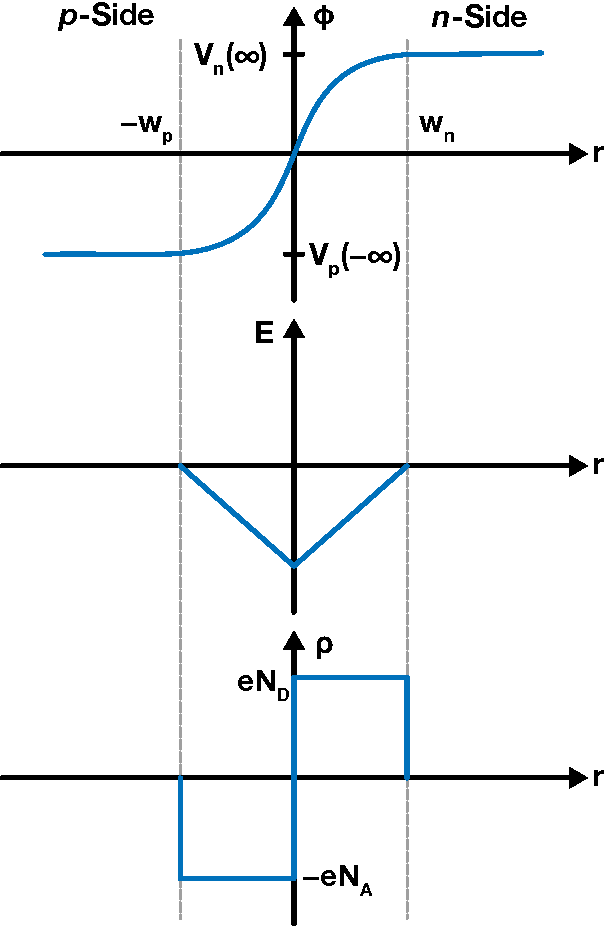
\includegraphics[width=0.5\textwidth]{Figures/Schematics/Theoretical Foundations/p-n-junction-potential-efield-charge-carrier-density.pdf}
	\caption{Schematic illustration of the electrostatic potential $\phi\left(r\right)$, the electric field $E\left(r\right)$ and the charge carrier density $\rho\left(r\right)$ across a $p$-$n$-junction, where the dashed lines indicate the width of the depletion region from $-w_p$ to $w_n$ \cite{Hook1991,Piprek2003,Kittel2004}.}
	\label{fig:p-n-junction-potential-efield-charge-carrier-density}
\end{figure}
This bending of the electron bands can likewise be observed with a reverse bias applied (positive terminal connected to the $n$-side and negative terminal to the $p$-side), where the flow of majority charge carriers across the diode is drastically reduced through the increased potential barrier, effectively minimizing the charge flow \cite{Hook1991,Piprek2003,Kittel2004}.
\section{Numerical Modeling of Semiconductor Nanostructures} \label{sec:nextnano-modeling}
Over the past 50 years, unprecedented technological advances have made large scale modeling and simulation of sophisticated nanoscale structures and electrical circuits computationally and economically viable \cite{More1965,Bank1990,Smith1997,Flamm2003,Wachutka2004,Mack2011,Leiserson2020}. On this basis, the \emph{nextnano} software package\footnote{A software license was graciously provided by Dr.~Stefan Birner for the purpose of this work.} enables the characterization of various physical and optical properties of such nanodevices by solving the Schrödinger-Poisson-current equation and 8-band $\vb{k}\cdot\vb{p}$~model self-consistently \cite{Birner2006,Trellakis2006,Birner2007}, as described in detail in \cref{ssec:k-p-method,ssec:schrödinger-current-poisson-equation,ssec:numerical-approaches}.
\subsection{\boldmath\texorpdfstring{$\vb{k}\cdot\vb{p}$}{k·p} Perturbation Theory} \label{ssec:k-p-method}
While various different methods and approximations for determining the band structure and related physical and optical properties of solids have been developed throughout the years, such as density functional theory \cite{Hellmann1935,Hohenberg1964,Kohn1965,Topp1973,Langreth1983,Becke1988,Perdew1992}, Green's functions methods and the Korringa-Kohn-Rostoker method \cite{Korringa1947,Kohn1954,Dupree1961,Morgan1966,Beeby1967,Madelung1967,Zeller1995,Wildberger1997,Papanikolaou2002,Buth2005,Jiang2011}, the tight-binding model \cite{Slater1954,Kwon1994,Lenosky1997,Schulz2005}, dynamic mean field theory \cite{Georges1992,Georges1996,Kotliar2004,Vollhardt2010}, the Kronig-Penney model \cite{Kronig1931,Singh1983,Cho1987,Yuh1988}, or the Hubbard model \cite{Hubbard1963-I,Hubbard1964-II,Hubbard1964-III}, this section focuses on the (multi-band) $\vb{k}\cdot\vb{p}$~method, as used by \emph{nextnano} \cite{Birner2006,Trellakis2006,Birner2007}. One advantage of this approach is that the band structure over the whole Brillouin zone can be extrapolated from the energy of the zone's center, yielding analytical expressions for the band dispersion and effective masses around high symmetry points \cite{Kittel1987,Piprek2003,Yu2010}.

Using the $\vb{k}\cdot\vb{p}$~approximation, the band structure of solids around $\vb{k}_0$\footnote{Usually the $\Gamma$-Point where $\vb{k}_0 = 0$ \cite{Kittel1987,Piprek2003,Yu2010}.}, for which the solution of the Schrödinger equation is known, can be extrapolated by a perturbation theory approach \cite{Kittel1987,Piprek2003,Yu2010}. Inserting the Bloch functions~\labelcref{eq:bloch-theorem} into the single-electron Schrödinger equation yields:
\begin{equation}
  \left[ \frac{p^2}{2m_0} + \frac{\hbar}{m_0}\vb{k}\cdot\vb{p} + eV\left(\vb{r}\right)\right]u_{n,\vb{k}}\left(\vb{r}\right) = \left[E_n\left(\vb{k}\right) - \frac{\hbar^2k^2}{2m_0}\right]u_{n,\vb{k}}\left(\vb{r}\right),
\end{equation}
allowing for the linear expansion of the Bloch functions $u_{n,\vb{k}}\left(\vb{r}\right)$ of the solution $u_{n,\vb{k}_0}\left(\vb{r}\right)$ at the known wave vector $\vb{k}_0$:
\begin{equation}
  u_{n,\vb{k}}\left(\vb{r}\right) = \sum_m a_{n,m} u_{m,\vb{k}_0}\left(\vb{r}\right),
\end{equation}
with the expansion coefficients $a_{n,m}$ \cite{Kittel1987,Piprek2003,Yu2010}. With this, the Hamiltonian can be simplified:
\begin{equation}
  H = H_0 + H_{\vb{k}}',
\end{equation}
with the unperturbated Hamiltonian $H_0$ and the perturbation $H_{\vb{k}}'$, giving the $\vb{k}\cdot\vb{p}$~method its distinctive name \cite{Kittel1987,Piprek2003,Yu2010}.

In the non-degenerate case, the eigenfunctions $u_{n,\vb{k}}\left(\vb{r}\right)$ and eigenvalues $E_{n,\vb{k}}$ can be expanded to second order in $\vb{k}$, yielding:
\begin{align}
  u_{n,\vb{k}}\left(\vb{r}\right) &= u_{n,\vb{k}_0}\left(\vb{r}\right) + \frac{\hbar}{m_0}\sum_{n'\neq n} \frac{\mel**{u_{n,\vb{k}_0}\left(\vb{r}\right)}{\vb{k}\cdot\vb{p}}{u_{n',\vb{k}_0}\left(\vb{r}\right)}}{E_{n,\vb{k}_0} - E_{n',\vb{k}_0}} u_{n',\vb{k}_0} \\
  E_{n,\vb{k}} &= E_{n,\vb{k}_0} + \frac{\hbar^2k^2}{2m_0} + \frac{\hbar^2}{m_0^2}\sum_{n' \neq n} \frac{|\mel**{u_{n,\vb{k}_0}\left(\vb{r}\right)}{\vb{k}\cdot\vb{p}}{u_{n',\vb{k}_0}\left(\vb{r}\right)}|^2}{E_{n,\vb{k}_0} - E_{n',\vb{k}_0}},
\end{align}
where the linear terms in $k$ vanish \cite{Kittel1987,Piprek2003,Yu2010}. The energy $E_{n,\vb{k}}$ can thus be rewritten for small~$k$:
\begin{equation}
  E_{n,\vb{k}} = E_{n,\vb{k}_0} + \frac{\hbar^2k^2}{2_m^\ast},
\end{equation}
from which the effective mass $m^\ast$ can be derived \cite{Kittel1987,Piprek2003,Yu2010}:
\begin{equation}
  \frac{1}{m^\ast} = \frac{1}{m_0} + \frac{1}{m^2k^2} \sum_{n' \neq n} \frac{|\mel**{u_{n,\vb{k}_0}\left(\vb{r}\right)}{\vb{k}\cdot\vb{p}}{u_{n',\vb{k}_0}\left(\vb{r}\right)}|^2}{E_{n,\vb{k}_0} - E_{n',\vb{k}_0}}.
\end{equation}
For a more accurate description of the band structure, it is necessary to consider the spin-orbit interaction, for which the Hamiltonian becomes:
\begin{equation}
  H_k' = \frac{p^2}{2m_0} + \frac{\hbar}{m_0}\vb{k}\cdot\vb{p} + \frac{\hbar^2k^2}{2m_0} + V\left(\vb{r}\right) + \frac{\hbar}{4m_0^2c^2} \left(\grad V\left(\vb{r}\right) \cp \left(\vb{p} + \hbar\vb{k}\right)\right) \cdot \vb{\sigma},
\end{equation}
with the three Pauli matrices $\vb{\sigma} = \left(\sigma_x, \sigma_y, \sigma_z\right)$ \cite{Kittel1987,Piprek2003,Yu2010}.

Separating the electron bands into two groups $A$ and $B$ allows for the derivation of a finite dimensional Hamiltonian \cite{Loewdin1951,Kane1966}, where the number of bands in group $A$ gives rise to the different multi-band $\vb{k}\cdot\vb{p}$~methods \cite{Luttinger1955,Luttinger1956}, with the most commonly used ones being the 4-band\footnote{The 4~bands are: conduction~(C), heavy hole~(HH), light hole~(LH) and split-off~(SO) \cite{Deen2012,Piprek2003}.} method \cite{Deen2012,Piprek2003}, the 6-band method \cite{Chao1992,Zhukov2013} and the 8-band method \cite{Kane1957,Chuang1996,Bahder1990,Enders1995}.
\subsection{Schrödinger-Poisson-Current Equation} \label{ssec:schrödinger-current-poisson-equation}
A description of the electrostatic potential of semiconductors is given by the Poisson equation:
\begin{equation}
  \grad\left[\epsilon\left(\vb{r}\right)\grad \phi \left(\vb{r}\right)\right] = -\rho\left(\vb{r}\right),
\end{equation}
from which the charge density can be derived:
\begin{equation}
  \rho\left(\vb{r}\right) = e \left[p\left(\vb{r}\right) - n\left(\vb{r}\right) + N_D\left(\vb{r}\right) - N_A\left(\vb{r}\right)\right],
\end{equation}
with the electron and hole concentration $n\left(\vb{r}\right)$ and $p\left(\vb{r}\right)$ \cite{Li2004,Birner2006}.

A unique solution within a given region $\mathcal{R}$ can be obtained through specific boundary conditions:
\begin{alignat}{3}
  \phi\left(\vb{r}\right) \rvert_{\vb{r} \in \partial \mathcal{R}} &= f\left(\vb{r}\right) &\qquad\text{Dirichlet}&\\
  \partial_{\vb{n}}\phi\left(\vb{r}\right)\rvert_{\vb{r} \in \partial \mathcal{R}} &= g\left(\vb{r}\right) &\qquad\text{von Neumann}&,
\end{alignat}
where the given functions $f\left(\vb{r}\right)$ and $g\left(\vb{r}\right)$ lie on the boundary of $\mathcal{R}$ and $\vb{n}$ denotes the normal with regard to the boundary $\partial \mathcal{R}$ \cite*{Jomaa2005,Ma2013}.

The carrier transport under an applied bias can be described with a quantum-drift-diffusion model through the Boltzmann equations, yielding the current density:
\begin{equation}
  \vb{j}\left(\vb{r}\right) = \mu\left(\vb{r}\right) n\left(\vb{r}\right) \grad E_F\left(\vb{r}\right) \quad ; \quad \div \vb{j}\left(\vb{r}\right) = 0,
\end{equation}
with the carrier density $n\left(\vb{r}\right)$, the mobility $\mu\left(\vb{r}\right)$ and the quasi Fermi level $E_F\left(\vb{r}\right)$ \cite{Sabathil2002,Birner2007}. Alternatively, a contact block reduction method can be used, which does not include any scattering or decoherence \cite{Mamaluy2003,Mamaluy2005}.
\subsection{Numerical Approaches} \label{ssec:numerical-approaches}
\emph{nextnano}, like all other computer-based methods, needs to find numerical techniques and approaches to solve analytical problems. All equations that need solving within \emph{nextnano} are partial differential equations, using box integration finite differences for discretization \cite{Trellakis2006}. The strain of the system can be calculated with a continuum elasticity approach, whereas the (conduction and valence) band edges are derived from band offsets and deformation potential theory, after which the coupled multi-band Schrödinger, Poisson and current equations can be solved self-consistently \cite{Birner2006,Birner2007}. Iterative methods \cite{Greenbaum1997,Bai2000} such as the preconditioned conjugate gradient method \cite{Hestenes1952}, the preconditioned composite step conjugate gradient method, or the preconditioned composite step biconjugate gradient method \cite{Lanczos1952,Bank1993} and incomplete Cholesky factorization \cite{Meijerink1977} or the Dupont-Kendall-Rachford method \cite{Dupont1968} as a preconditioner can be utilized, along with a predictor-corrector method based on the Newton-Raphson method with inexact line search \cite{Trellakis1997}, when solving the coupled Schrödinger and Poisson equations \cite{Birner2006}. Eigenvalues can be found using the Lanczos or Arnoldi iteration methods \cite{Greenbaum1997,Bai2000,Birner2006}, along with the \emph{ARPACK} software package with an optimized preconditioner using Chebyshev polynomials \cite{Lehoucq1998,Birner2006}, or in the case of non-extreme eigenvalues using the Jacobi-Davidson method \cite{Sleijpen1996}. In order to guarantee the hermiticity of the Hamiltonians, \emph{nextnano} employs a combination of forward and backward differentiation \cite{Birner2006}. For the case of metal oxide surfaces, the site-binding model allows for the consideration of interface reactions \cite{Bergveld1970,Healy1978,Bayer2005,Birner2006}.

Although numerical simulations are in excellent agreement with the theoretically expected behavior of the modeled specimens, they often fail to accurately incorporate various real-world effects observed during measurements (e.\,g.\ surface effects resulting from ion-induced defects during the specimen preparation stage \cite{Twitchett2002,Beleggia2003,Cooper2006,Cooper2007,Twitchett-Harrison2007,Cooper2009,Somodi2013,Yazdi2015}), necessitating the need for an alternative model that takes these effects into account.
\section{Off-Axis Electron Holography} \label{sec:electron-holography}
Science's pursuit of investigating ever-smaller micro- and nanoscale structures has also led to a need for correspondingly high-resolution observation and imaging methods. Driven by these demands for an imaging method that is vastly superior to classical light microscopy in regard to angular resolution, transmission electron microscopy~(TEM), and by that extent electron holography (EH), has emerged as one of the most pivotal\footnote{For his invention of the first TEM in 1931 \cite{Ruska1932-I,Ruska1932-II}, Ernst~Ruska was awarded the Nobel~Prize in 1986 \cite{Ruska1986,Robinson1986}, an achievement shared by Dennis~Gabor, who likewise received the Nobel~Prize in 1971 \cite{Gabor1971} for his invention of electron holography in 1947 \cite{Gabor1948,Gabor1949}.} methods over the last 90~years \cite{Curry2006,Kisielowski2008,Deepak2015,Franken2017,Li2019}. Particularly for the observation of electrostatic potential distribution in nanoelectronic devices, electron holography, with its separate access to amplitude and phase information of reconstructed electron waves, provides a well established imaging method \cite{Lichte1986,Tonomura1987,Cowley1992,DuninBorkowski2004}, as described in detail in \cref{ssec:electron-interference,ssec:electron-holography-electrostatic-potential,ssec:electron-holography-pn-junctions}.
\subsection{Electron Interference} \label{ssec:electron-interference}
The relative phase distribution of an electron wave propagating through a TEM can be determined from the interference pattern, produced by superimposing the modulated object wave $\psi_{\mathit{obj}}\left(\vb{r}\right)$ propagating through the specimen and the unmodulated reference wave $\psi_{\mathit{ref}}\left(\vb{r}\right)$ propagating undisturbed through a nearby vacuum region (\cref{fig:TEM-off-axis-holography-setup}):
\begin{equation}
  \psi_{\mathit{obj}}\left(\vb{r}\right) = a_{\mathit{obj}}\left(\vb{r}\right)e^{i \varphi_{\mathit{obj}}\left(\vb{r}\right)} \quad ; \quad \psi_{\mathit{ref}}\left(\vb{r}\right) = a_{\mathit{ref}}\left(\vb{r}\right)e^{i \varphi_{\mathit{ref}}\left(\vb{r}\right)},
\end{equation}
where $a_{\mathit{obj}}\left(\vb{r}\right)$ and $a_{\mathit{ref}}\left(\vb{r}\right)$, and $\varphi_{\mathit{obj}}\left(\vb{r}\right)$ and $\varphi_{\mathit{ref}}\left(\vb{r}\right)$ are the respective amplitude and phase of the object and reference wave \cite{Voelkl1999,Lehmann2002,Lichte2008}.
\begin{figure}[H]
	\centering
	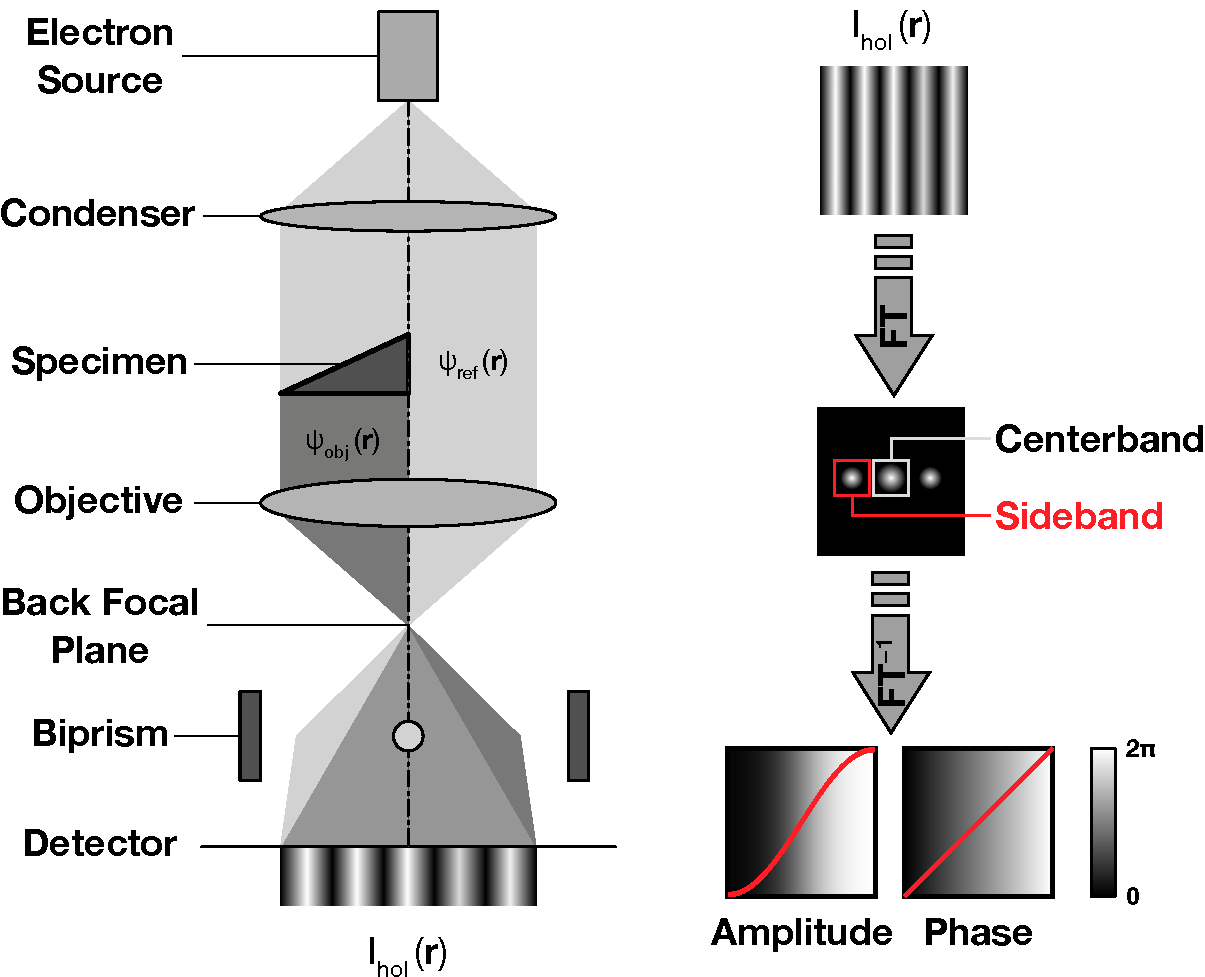
\includegraphics[width=0.8\textwidth]{Figures/Schematics/Theoretical Foundations/TEM-off-axis-holography-setup.pdf}
	\caption{\emph{Left:} Schematic illustration of the acquisition of an off-axis electron hologram in a TEM \cite{Lehmann1994,Voelkl1995,Voelkl1999,Lehmann2002,Lichte2008}. Part of electron wave propagates through the specimen, resulting in the modulated object wave ${\psi}_{\mathit{obj}}\left(\vb{r}\right)$, while the other part propagates through a nearby vacuum region, resulting in the unmodulated reference wave ${\psi}_{\mathit{ref}}\left(\vb{r}\right)$, ultimately creating an interference pattern after being superimposed through the deflection of a biprism \cite{Moellenstedt1956,Lehmann1994,Voelkl1995,Voelkl1999,Lehmann2002,Lichte2008}. \emph{Right:} Schematic illustration describing the reconstruction process of an off-axis electron hologram \cite{Lehmann1994,Voelkl1995,Voelkl1999,Lehmann2002,Lichte2008}. After the interference pattern is Fourier transformed, resulting in a centerband and two sidebands $\left(\pm 1\right)$, one of the two sidebands is inversely Fourier transformed, yielding the amplitude $a\left(\vb{r}\right)$ and the phase $\varphi\left(\vb{r}\right)$ (with their profiles indicated by the red curves) \cite{Lehmann1994,Voelkl1995,Voelkl1999,Lehmann2002,Lichte2008}.}
	\label{fig:TEM-off-axis-holography-setup}
\end{figure}
By coherently overlapping both electron waves under an angle $\beta$ through the deflection of a so called Möllenstedt biprism \cite{Moellenstedt1956}, the desired hologram can be obtained:
\begin{equation}
	I_{\mathit{hol}}\left(\vb{r}\right) = 1 + a^2\left(\vb{r}\right) + 2\mu a\left(\vb{r}\right)\cos(2\pi \vb{q}_c\vb{r} + \varphi\left(\vb{r}\right) + \theta\left(\vb{r},\vb{q}_c\right)),
\end{equation}
with the amplitude $a\left(\vb{r}\right)$ and the phase $\varphi\left(\vb{r}\right) = {\varphi}_{\mathit{obj}}\left(\vb{r}\right) - {\varphi}_{\mathit{ref}}\left(\vb{r}\right)$ of the reconstructed electron wave ${\psi}_{\mathit{el}}\left(\vb{r}\right)$, the carrier frequency of the interference fringes $\abs{\vb{q}_c} = {\beta}/{\lambda}$\footnote{For his introduction of the wavelength of particles $\lambda = h / p$ in 1924 \cite{BrogliePhD1924}, Louis~de~Broglie was awarded the Nobel~Prize in 1929 \cite{Broglie1929}.}, the corresponding contrast $\mu = \left(I_{\mathit{max}}\left(\vb{r}\right) - I_{\mathit{min}}\left(\vb{r}\right)\right) / \left(I_{\mathit{max}}\left(\vb{r}\right) + I_{\mathit{min}}\left(\vb{r}\right)\right)$ \cite{Voelkl1999,Lehmann2002,Lichte2008} and an additional phase modulation $\theta\left(\vb{r}, \vb{q}_c\right)$ \cite{LehmannPhD1997}. The resulting hologram therefore contains information about the amplitude in the form of contrast modulation and the phase in the form of interference fringe bending \cite{Voelkl1999,Lehmann2002,Lichte2008}.

The above mentioned distortion-induced phase modulations $\theta\left(\vb{r}, \vb{q}_c\right)$, representing the microscope's non-isoplanatic aberrations, make the recording of an empty hologram, where the specimen is removed and both the object and reference wave propagate through the vacuum region, directly after each object hologram necessary, allowing for the normalization of the amplitude and resulting in \cite{Voelkl1999,Lehmann2002,Lichte2008}:
\begin{equation}
  I_{\mathit{emp}}\left(\vb{r}\right) = 1 + 2\mu \cos(2\pi \vb{q}_c \vb{r} + \theta\left(\vb{r}, \vb{q}_c\right)).
\end{equation}
Being a two-step process, electron holography requires the subsequent numerical reconstruction of the recorded hologram \cite{Voelkl1999,Lehmann2002,Lichte2008}. For this purpose, the Fourier transform of the electron hologram can be calculated \cite{Lehmann1994,Voelkl1995,Voelkl1999,Lehmann2002,Lichte2008}:
	\begin{alignat}{3}
		\mathcal{F}\left\{ I_{\mathit{hol}}\left(\vb{r}\right) \right\} &= \mathcal{F}\left\{ 1 + a^2\left(\vb{r}\right) \right\} &\qquad\text{Centerband}& \notag \\
		&+ \mu \mathcal{F}\left\{ a\left(\vb{r}\right)e^{i\left(\varphi\left(\vb{r}\right) + \theta\left(\vb{r},\vb{q}_c\right)\right)} \right\} * \delta\left(\vb{q} - \vb{q}_c\right) &\quad\text{Sideband $\left(+1\right)$}& \notag \\
		&+ \mu \mathcal{F}\left\{ a\left(\vb{r}\right)e^{-i\left(\varphi\left(\vb{r}\right) + \theta\left(\vb{r},\vb{q}_c\right)\right)}\right\} * \delta\left(\vb{q} + \vb{q}_c\right) &\qquad\text{Sideband $\left(-1\right)$}&.
	\end{alignat}
Subsequently centering and isolating one\footnote{Usually the sideband in reference wave direction.} of the two sidebands and calculating the inverse Fourier transform $\mathcal{F}^{-1}$ results in the reconstructed electron wave (\cref{fig:TEM-off-axis-holography-setup}):
\begin{equation}
	{\psi}_{\mathit{el}}\left(\vb{r}\right) = \mu a\left(\vb{r}\right)e^{i\varphi\left(\vb{r}\right)},
\end{equation}
where the phase $\varphi\left(\vb{r}\right)$ is $2\pi$-wrapped to an interval of $\interval{-\pi}{\pi}$ \cite{Lehmann1994,Voelkl1995,Voelkl1999,Lehmann2002,Lichte2008}.

It should further be noted that although the reference wave is often assumed to be free from perturbations, various stray field effects in real-world experimental setups, especially in electrical biasing EH, necessitate shielding against these unwanted modulations \cite{Wagner2019,Wagner2022}.

\subsection{Electron Holography of the Electrostatic Potential} \label{ssec:electron-holography-electrostatic-potential}
The potential distribution of a specimen is encoded in its object hologram, where, in the absence of a magnetic vector potential, the object phase can derived from the Wentzel-Kramer-Brillouin approximation:
\begin{equation}
  \label{eq:electron-holography-electrostatic-potential}
  \varphi_{\mathit{obj}}\left(\vb{r}\right) = \frac{\pi}{\lambda E}\int\limits_{L} \phi\left(\vb{r}\right) \dd{z} = \sigma \phi_{\mathit{proj}}\left(\vb{r}\right),
\end{equation}
with a straight line integration path $L$ parallel to the $z$-axis (i.\,e.\ the electron beam direction), an acceleration voltage dependent interaction constant $\sigma = \pi / \lambda E$ and the projected electric potential $\phi_{\mathit{proj}}\left(\vb{r}\right)$ \cite{Voelkl1999,Lehmann2002,Lichte2008}. From this phase shift, the mean inner potential can be derived:
\begin{equation}
  \label{eq:electron-holography-MIP}
  \varphi_{\mathit{obj}}\left(\vb{r}\right) = \sigma \phi_{\mathit{MIP}}\left(\vb{r}\right) t
\end{equation}
with the intrinsic mean inner potential $\phi_{\mathit{MIP}}\left(\vb{r}\right)$, given by the electrostatic potential of the nuclei, and the specimen thickness $t$ \cite{Voelkl1999,Lehmann2002,Lichte2008}. This possibility to extract information about the electrostatic potential distribution in specimens, especially when the amplitude profile is unmodulated and offers no significant insight into the investigated specimen, makes electron holography an excellent method for in situ investigations of semiconductor nanodevices (i.\,e.\ electrical biasing electron holography) \cite{Tonomura1987,Lehmann2002,Lichte2008}, as described in the following \cref{ssec:electron-holography-pn-junctions}.
\subsection[Electron Holography of \texorpdfstring{$p$-$n$}{\textit{p}-\textit{n}}-Junctions]{Electron Holography of $\boldsymbol{p}$-$\boldsymbol{n}$-Junctions} \label{ssec:electron-holography-pn-junctions}
Based on \cref{eq:electron-holography-electrostatic-potential,eq:electron-holography-MIP}, the phase shift of a $p$-$n$-junction is given by:
\begin{equation}
  \label{eq:EH-phase-shift-specimen}
  \varphi\left(\vb{r}, U_{\mathit{ext}}\right) = \sigma \left[\phi_{\mathit{MIP}}\left(\vb{r}\right)\left(t_{\mathit{act}} + 2t_0\right) + \phi_{\mathit{pn}}\left(\vb{r}, U_{\mathit{ext}}\right)t_{\mathit{act}}\right],
\end{equation}
with the electrostatic potential of the $p$-$n$-junction $\phi_{\mathit{pn}}\left(\vb{r}, U_{\mathit{ext}}\right)$ and the specimen thickness $t$, which is made up of an electrically inactive\footnote{Recent investigations have shown that the electrically inactive boundary layer across the specimen does indeed contribute to the measured phase shift \cite{Wagner2022}.} boundary layer $t_0$ and an electrically active layer $t_{\mathit{act}}$ \cite{Frabboni1987,Twitchett2002,Cooper2006,Cooper2007,Cooper2009,He2013,Yazdi2015}. Using the electrostatic potential, and by that extent the phase shift obtained through electron holography, the electric field $E_{\mathit{pn}}\left(r, U_{\mathit{ext}}\right)$ and charge carrier density $\rho\left(r, U_{\mathit{ext}}\right)$ can be derived using Poisson's equation \cite{Frabboni1987,Twitchett2002,Yazdi2015}.

As described in \cref{ssec:band-structure-p-n-junctions}, the electric properties of a $p$-$n$-junction, such as the phase jump (or potential step) $\Delta \varphi_{\mathit{pn}}\left(U_{\mathit{ext}}\right)$, depend on the applied bias $U_{\mathit{ext}}$, with electric stray fields below and above the specimen leading to an additional phase shift that extend into the vacuum reference region \cite{Frabboni1987,Twitchett2002,Yazdi2015}.

The above detailed description of the electrostatic potential assumes a constant distribution in $z$-direction (i.\,e.\ the electron beam direction), which is often not the case for real-world measurements \cite{Twitchett-Harrison2007,Wagner2019}. Electron tomography, being a projective measurement method, is able to resolve this additional information in $z$-direction, as detailed in the following \cref{sec:electron-tomography}.

\section{Electron Tomography} \label{sec:electron-tomography}
Tomographic reconstruction is an imaging method that uses $k$ $\left(n - 1\right)$-dimensional projections of an object of interest to create a $n$-dimensional map \cite{Ramm1996,Herman2009,Kuchment2014}. The mathematical foundation for tomographic reconstructions was given by Johann Karl August Radon in 1917 \cite{Radon1917}, after whom the corresponding (inverse) Radon transform is named.

Given a 2D function $f\left(x, z\right)$, the integral along the path $L$ is given by:
\begin{equation}
  \label{eq:2D-radon-transform}
  \hat{f}_{\alpha} \left(x\right) = \int \limits_{L} f\left(x, z\right) \dd{z},
\end{equation}
where $\alpha$ describes the direction along which the path $L$ runs parallel to the $z$-axis (i.\,e.\ the electron beam direction) \cite{Ramm1996,Herman2009,Kuchment2014}. This continuous accumulation of 1D~projections towards a 2D~function $\hat{f}\left(\alpha, l\right)$ (i.\,e.\ the Radon transform) yields the so called sinogram \cite{Ramm1996,Herman2009,Kuchment2014}.

The projection-slice theorem further states that the $\left(n - 1\right)$-dimensional projection of a $n$-dimensional function in real space corresponds to a $\left(n - 1\right)$-dimensional cut through the origin of the $n$-dimensional Fourier transform in Fourier space:
\begin{equation}
  \hat{F}_{\vb{\xi}} \left(g\right) = \iint \limits_{-\infty}^{+\infty} F\left(\vb{\hat{g}'}\right) \delta \left(\vb{\hat{g}'} - g \vb{\hat{\xi}}\right) \dd[2]{g'},
\end{equation}
where $F\left(\vb{\hat{g}'}\right)$ is the 2D~Fourier transform of the 1D~function $f\left(\hat{\vb{r}}\right)$ and $\hat{\vb{\xi}} = \left[\cos\left(\alpha\right), \sin\left(\alpha\right)\right]^\intercal$ \cite{Ramm1996,Herman2009,Kuchment2014}.

The reconstruction of the original image from the sinogram constitutes an inverse problem \cite{Ramm1996,Herman2009,Kuchment2014}. Given infinite angular resolution, an inverse Radon transform of the sinogram yields a perfect reconstruction that is identical to the original image \cite{Ramm1996,Herman2009,Kuchment2014}. Since infinite resolution is not feasible with current experimental methods, various reconstruction approaches have been developed over the years \cite{Ramm1996,Herman2009,Kuchment2014}. One of the most common techniques is the so called filtered (or weighted) back-projection, where each 1D~projection is back-projection against its projection direction and summed up:
\begin{equation}
  \tilde{F}\left(\vb{\hat{g}}\right) = \iint \limits_{-\infty}^{+\infty} F\left(\vb{\hat{g}'}\right) \delta \left(\vb{\hat{g}'} - g \vb{\hat{\xi}}\right) \dd{\vb{\hat{\xi}}} \dd[2]{g'} = \frac{F\left(\vb{\hat{g}}\right)}{\lvert g \rvert},
\end{equation}
where $\lvert g \rvert$ is the weighting filter caused by the overemphasis on low spatial frequencies in Fourier space \cite{Ramm1996,Herman2009,Kuchment2014}. This improper weighting of low spacial frequencies can be partially compensated for by a suitable filter (e.\,g.\ ramp, Hann, Gaussian), lessening the observed smearing in the reconstructed image \cite{Ramm1996,Herman2009,Kuchment2014}.

An alternative approach is the iterative reconstruction, where an algorithm starts with an assumed image and tries to minimize the difference between the current computed reconstruction and the original image \cite{Ramm1996,Herman2009,Kuchment2014}. This approach, while sometimes more accurate, is usually computationally more expensive \cite{Ramm1996,Herman2009,Kuchment2014}.

Further limitations arise not only from a limited angular range that is smaller than the ideal $\alpha = \pm \SI{90}{\degree}$ (i.\,e.\ missing wedge) \cite{Ramm1996,Herman2009,Kuchment2014}, but also from a detector that captures an region of interest smaller than the entire object (i.\,e.\ interior radon transform) \cite{Maass1992,Pan2005,DaSilva2018}.

In a TEM, the 2D~projections of the 3D~specimen are given by the electron beam propagating through the specimen towards the detector, where recent developments have demonstrated electron tomography with atomic spacial resolution \cite{Scott2012,Miao2016,Yang2017}. In detail, the 2D~phase shift of a 3D~potential distribution for a constant tilt angle $\alpha$ is given according to \cref{eq:electrostatic-poisson-green} \cite{Wolf2014,Lubk2014}:
\begin{equation}
  \varphi_{\mathit{obj}}\left(\vb{r}, \alpha \right) = \sigma \int\limits_{L\left(\alpha\right)} \phi\left(\vb{r}\right) \dd{z}.
\end{equation}

\chapter{Experimental Methods} \label{chap:experimental-methods}
The following chapter presents the methods used for investigating the physical properties of semiconductor nanostructure specimens using off-axis electron holography, including their preparation, numerical modeling and the automation of the measurement and reconstruction process.
\section{Specimen Preparation} \label{sec:specimen-preparation}
Following the rapid development of integrated circuits (particularly in regards to their transistor density) in the 1980s and onwards, focused ion beam (FIB) milling has emerged as one of the most well established techniques for the analysis of such nanoscale structures \cite{Orloff2003,Giannuzzi2005}. Resembling a scanning electron microscopes (SEM), the FIB substitutes the focused electron beam with a focused ion beam produced by high electric fields \cite{Orloff2003,Giannuzzi2005}. While liquid metal ion sources (LIMS), especially Ga ion sources, comprise a large share of currently available instruments, gas field ion sources (GFIS) using plasma beams of noble gases, such as Xe, have become more widespread in recent time \cite{Orloff2003,Giannuzzi2005,Burnett2016}. The FIB's inherently destructive behavior towards the specimen by ion implantation into the specimen surface makes it a suitable tool for high precision milling \cite{Orloff2003,Giannuzzi2005}. This ability to remove selected areas with a precision of $\SI{10}{\nm}$ or less has established FIB milling as an viable and practical technique that goes far beyond TEM specimen preparation \cite{Orloff2003,Giannuzzi2005}.

The following \cref{ssec:specimen-preparation-capacitor,ssec:specimen-preparation-pn-junction} give a brief insight into the preparation of a coplanar capacitor and $p$-$p^+$-$n^+$-junction specimen using a FEI™ Helios NanoLab 600 DualBeam, consisting of both a SEM and a FIB.
\newpage
\subsection{Coplanar Capacitor} \label{ssec:specimen-preparation-capacitor}
The first specimen, a coplanar capacitor, is used a reference specimen for evaluation purposes due to its well known geometry, electric behavior and potential distribution.

The capacitor was produced utilizing FIB milling of an Au~film (roughly $\SI{25}{\um} \times \SI{16}{\um} \times \SI{3}{\um}$), which was transferred using an Oxford Instruments™ OmniProbe micromanipulator and contacted via FIB induced Pt~deposition onto a Protochips™ MEMS-based carrier FIB-E-Chip (\cref{fig:capacitor-specimen-FIB-preperation-SEM}a).
\begin{figure}[H]
	\centering
	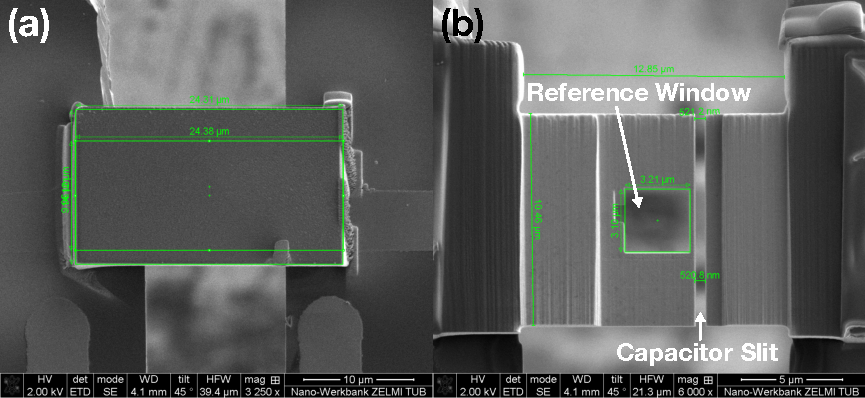
\includegraphics[width=\textwidth]{Figures/Specimen/Capacitor/capacitor-specimen-FIB-preperation-SEM.pdf}
	\caption{SEM images of the coplanar capacitor with (a) the placement/contacting (FIB induced Pt~deposition) of the Au~film and (b) the finished processed capacitor with a reference window in the left electrode.}
	\label{fig:capacitor-specimen-FIB-preperation-SEM}
\end{figure}
In the area of interest, the Au~film was thinned to a thickness of approximately $\SI{500}{\nm}$, separated over the entire width of the film (parallel to the electrodes of the carrier chip) to a distance of approximately $\SI{500}{\nm}$, resulting in two free-standing coplanar electrodes, and fitted with a reference window of roughly $\SI{3}{\um} \times \SI{3}{\um}$ near the slit of the capacitor (\cref{fig:capacitor-specimen-FIB-preperation-SEM}b). This cutout serves as an almost undisturbed region for the reference wave to propagate through, since the conductive edge of the reference window acts like a Faraday cage, therefore shielding the reference wave from unwanted modulations, which are especially present in electric biasing EH \cite{Wagner2019,Wagner2022}.
\newpage
\subsection[\texorpdfstring{$p$-$p^+$-$n^+$}{\textit{p}-\textit{p}\textsuperscript{+}-\textit{n}\textsuperscript{+}}-Junction]{$\boldsymbol{p}$-$\boldsymbol{p^+}$-$\boldsymbol{n^+}$-Junction} \label{ssec:specimen-preparation-pn-junction}
The second specimen, a $p$-$p^+$-$n^+$-junction, was cut out from a Si~wafer using standard FIB procedures and placed (similar to the above described coplanar capacitor) onto the carrier chip (\cref{fig:pn-junction-specimen-FIB-preperation-SEM}a and b).
\begin{figure}[H]
	\centering
	\includegraphics[width=\textwidth]{Figures/Specimen/pn-Junction/pn-junction-specimen-FIB-preperation-SEM.pdf}
	\caption{SEM images related to the specimen preparation of the $p$-$p^+$-$n^+$-junction with (a) the electrode geometry of the FIB-E-Chip, (b) the transfer of the FIB cut-out using the micromanipulator, (c) the contacted TEM lamella featuring the $p$-$p^+$-$n^+$-junction and a reference window close to it and (d) a side view of the TEM lamella during the thinning and cleaning process.}
	\label{fig:pn-junction-specimen-FIB-preperation-SEM}
\end{figure}
The lamella was contacted (FIB induced Pt~deposition) in such a way that the interface of the junction sits parallel to free-standing electrodes of the carrier chip (\cref{fig:pn-junction-specimen-FIB-preperation-SEM}c). The finished specimen was thinned to a thickness of approximately $\SI{350}{\nm}$ and fitted with a reference window close to the $p^+$-$n^+$-junction (\cref{fig:pn-junction-specimen-FIB-preperation-SEM}d). Through this geometry, the diode current is directly guided through the lamella (and its surface) with externally applied bias.
\newpage
\section{Numerical Modeling} \label{sec:numerical-modeling}
In order to accurately interpret and understand the experimental results obtained from off-axis electron holography measurements of the above mentioned two specimens, 2D~numerical simulations were carried out using different finite element method (FEM) software packages.
\subsection{2D Modeling of the Specimen} \label{ssec:2d-modeling-specimen}
A half-modeling approach that utilities the axial symmetry of the specimens can be used to reduce the computational complexity of the simulations. Specifically, only half of the specimens and stray fields were simulated, which significantly reduced the amount of RAM and computation time needed to obtain results. In order to obtain physical quantities, such as the electrostatic potential or phase, from the simulated half-model, appropriate adjustments were made to account for the symmetry of the problems.

The coplanar capacitor was modeled using the \emph{ONELAB} software bundle \cite{Geuzaine2013}, consisting of \emph{Gmsh} (a FEM mesh generator) \cite{Geuzaine2009} and \emph{GetDP} (a discrete physical problem solver) \cite{Dular1998}. For this, two coplanar plates of thickness $t = \SI{250}{\nm}$ each were placed $d = \SI{480}{\nm}$ apart from each other, with the stray field extending into the vacuum below the specimen, for a total dimension of $\SI{5000}{\nm} \times \SI{8000}{\nm}$ (\cref{fig:specimen-capacitor-layout}). The two capacitor plates were biased with $-U_{ext}$ and $U_{ext}$ using Dirichlet boundary conditions, whereas the vacuum uses a von~Neumann boundary condition of zero.
\begin{figure}[H]
	\centering
	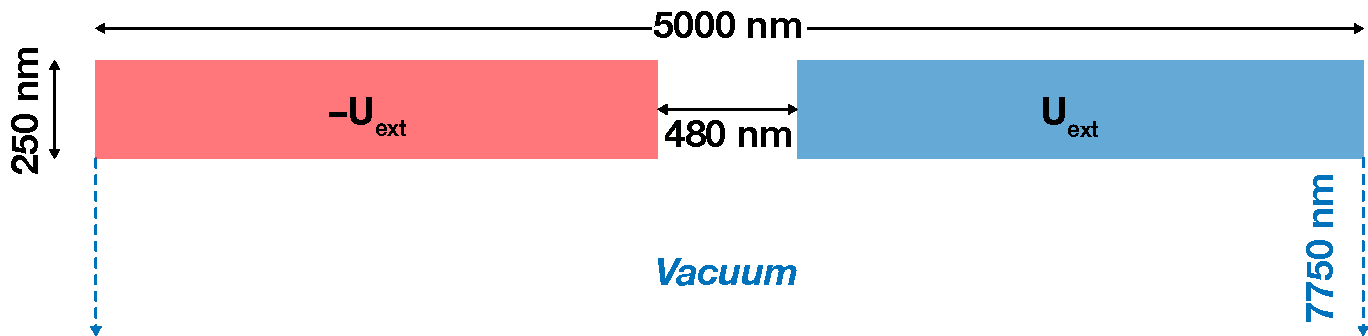
\includegraphics[width=\textwidth]{Figures/Specimen/Capacitor/specimen-capacitor-layout.pdf}
	\caption{Schematic illustration of the coplanar capacitor modeled using \emph{ONELAB}. The capacitor plates are spaced $d = \SI{480}{\nm}$ with a thickness of $t = \SI{250}{\nm}$ each, while the stray field extends into the vacuum region below the specimen for $\SI{7750}{\nm}$. Both capacitor plates are biased with $-U_{ext}$ and $U_{ext}$ using Dirichlet boundary conditions, whereas the vacuum uses a von~Neumann boundary condition of zero.}
	\label{fig:specimen-capacitor-layout}
\end{figure}
The $p$-$p^+$-$n^+$-junction was modeled using \emph{nextnano}. Here, three different Si~specimen regions with two different doping concentrations and equivalent lengths of $\SI{1000}{\nm}$ and thicknesses of $\SI{150}{\nm}$ each were defined (\cref{fig:specimen-nextnano-layout}). The weakly doped ($\SI[per-mode=power]{1e16}{\per\cubic\cm}$) $p$-region on the left features an abrupt transition to a heavily doped ($\SI[per-mode=power]{1e19}{\per\cubic\cm}$) $p^+$-region on the right, which in turn features an abrupt transition to an equivalently doped $n^+$-region. The specimen is further equipped with Schottky Pt contacts of $\SI{50}{\nm}$ width on both sides. The stray field extends below the specimen into the vacuum region for $\SI{2500}{\nm}$, while a temperature of $T = \SI{300}{\kelvin}$ was assumed.

To reduce the already high computational cost of the \emph{nextnano} simulation, the 2D~grid points were spaced only in the regions of interest (i.\,e.\ the $p$-$p^+$ and $p^+$-$n^+$-junction) with a distance of $\SI{1}{\nm}$. For the rest of the specimen and vacuum region, a grid point spacing of $\SI{10}{\nm}$ is sufficient, with no abrupt transition between the two spacing factors.
\begin{figure}[H]
	\centering
	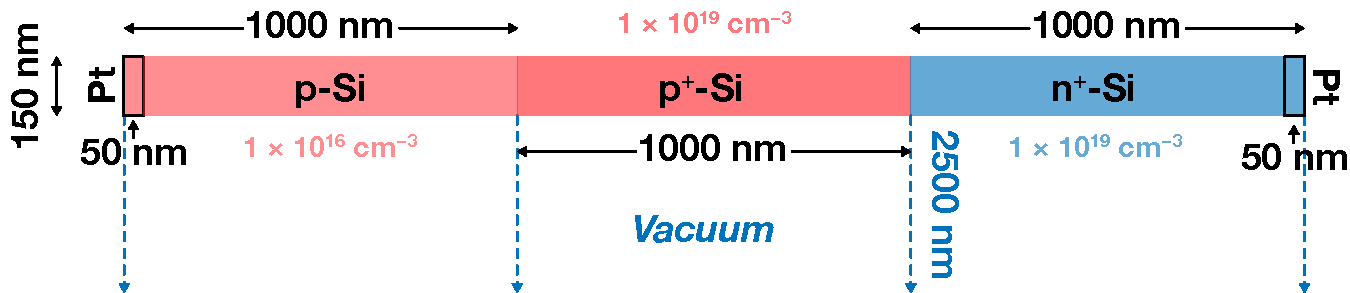
\includegraphics[width=\textwidth]{Figures/Specimen/pn-Junction/specimen-nextnano-layout.pdf}
	\caption{Schematic illustration of the $p$-$n$-junction modeled using \emph{nextnano}. All three specimen regions feature the same width of $\SI{1000}{\nm}$ and thickness of $\SI{150}{\nm}$ each, while the doping abruptly changes from $\SI[per-mode=power]{1e16}{\per\cubic\cm}$ to $\SI[per-mode=power]{1e19}{\per\cubic\cm}$ at the $p$-$p^+$-junction. Furthermore, Pt contacts are placed at both ends of the same with a width of $\SI{50}{\nm}$ each, whereas the stray field extends into the vacuum region for $\SI{7750}{\nm}$.}
	\label{fig:specimen-nextnano-layout}
\end{figure}
The coupled Schrödinger-Poisson-current equations were then solved iteratively, with the maximum number of iterations limited to $\num{10000}$.
\subsection{Simulated Potential and Phase} \label{ssec:FEM-simulated-potential-and-phase}
In order to extract the electrostatic potential, and with that the electric phase, from the above mentioned 2D~simulations, the output has to be parsed differently, depending on which software package was used.

For the \emph{ONELAB} simulation, the output of the simulation is the electrostatic potential with regards to the generated mesh of the corresponding physical problem. These mesh-based values can be exported to a generic text file using the \emph{CutParametric} plugin, where the required computation time and storage is heavily dependent on the global mesh size factor and number of points used for the parametric plane. This generic text file can then be parsed to \textsc{python}, where the electrostatic potential values are contained in the last 1D~column and reshaped to a proper 2D~grid according to the previously defined dimensions of the simulation. The object phase $\varphi_{\mathit{obj}}$ can be obtained by projecting the electrostatic potential in the electron beam propagation direction, i.\,e.\ by calculating the cumulative sum over all columns and extracting the last row. In addition, similar to the experimental measurement, a reference phase $\varphi_{\mathit{ref}}$ of the same width but different position can be subtracted from the object phase between the capacitor plates. Furthermore, the different contributions to the calculated phase $\varphi = \varphi_{\mathit{obj}} - \varphi_{\mathit{ref}}$ from the capacitor itself and the stray field can be adjusted through a pair of weighted thickness parameters influencing the projection of the electrostatic potential. At last, the calculated phase is multiplied with the interaction constant $\sigma$ (\cref{eq:electron-holography-electrostatic-potential}), where $\sigma = \SI{6.53}{rad \per \volt \um}$ for an acceleration voltage of $U_{\mathit{acc}} = \SI{300}{\kilo\volt}$ \cite{Beleggia2014}.

In comparison, \emph{nextnano} outputs the calculated electrostatic potential using the \emph{Visualization Toolkit} (i.\,e.\ \texttt{.vtr}) file format. Here, the \emph{nextnanopy} software package \cite{nextnanopy} provides an easy-to-use interface for parsing \emph{nextnano}'s output, where, in addition to the electrostatic potential, the Euclidian coordinates of the simulated grid points, along with their corresponding units, can be accessed. Similar to above, the object phase $\varphi_{\mathit{obj}}$ is calculated from the projection of the electrostatic potential through a cumulative sum over all columns (\cref{fig:flowchart-automatic-nextnano-post-processing}).
\begin{figure}[H]
	\centering
	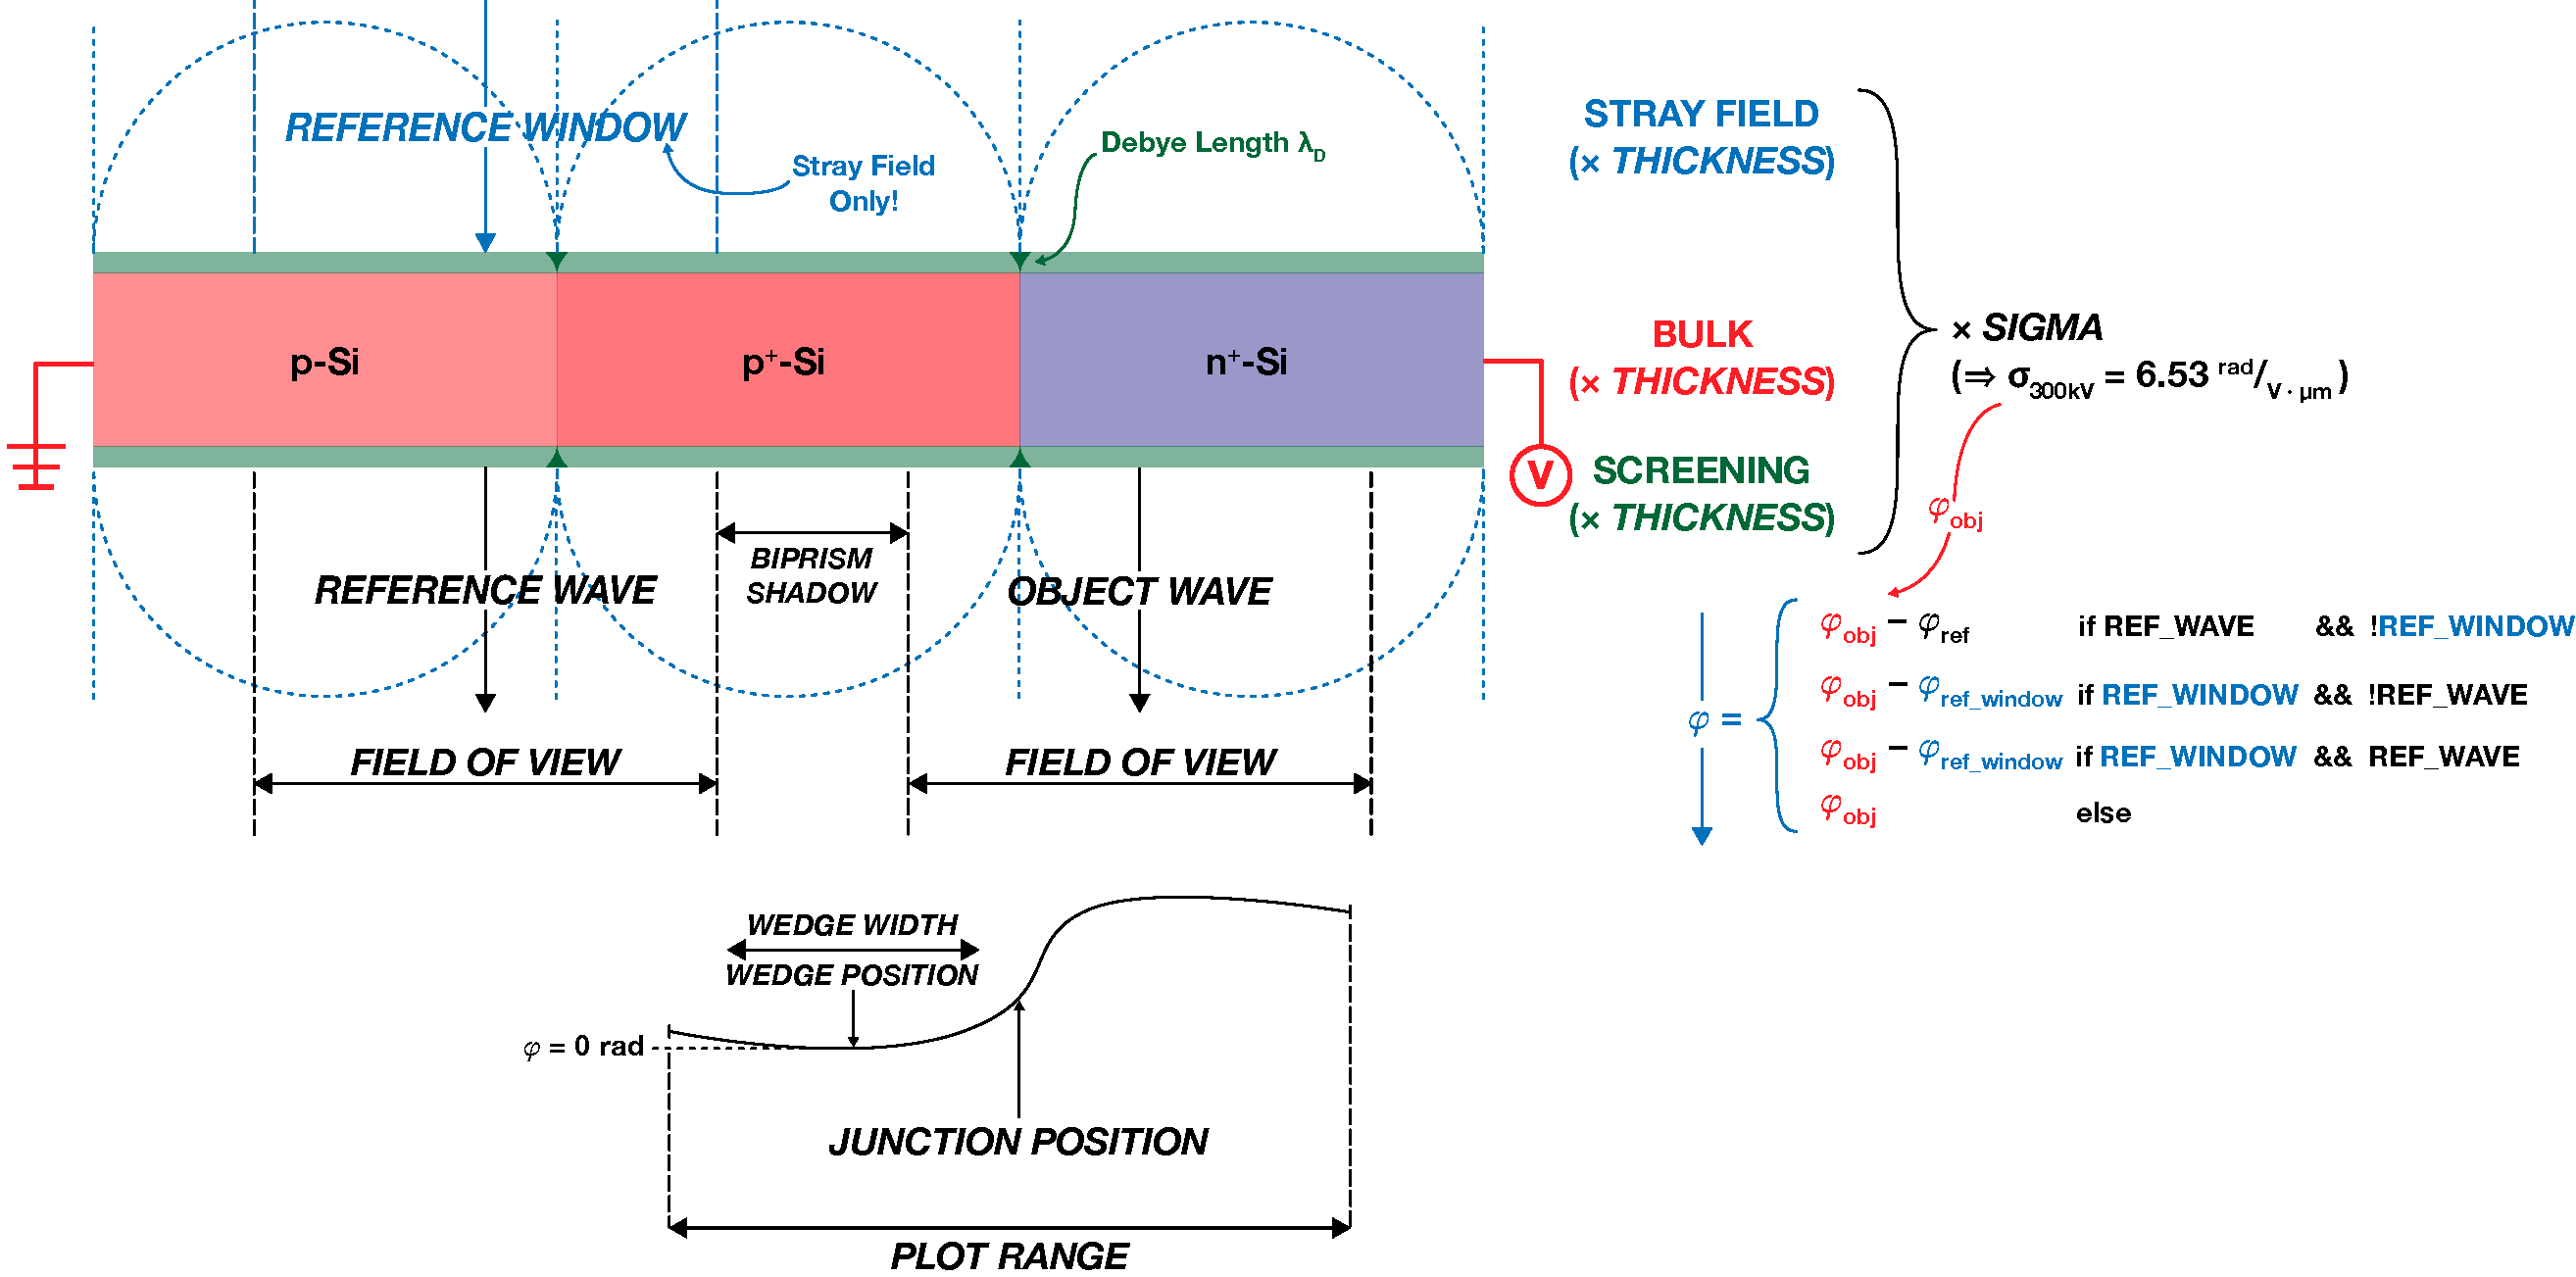
\includegraphics[width=\textwidth]{Figures/Schematics/Automation/flowchart-automatic-nextnano-post-processing.pdf}
	\caption{Schematic illustration detailing how the phase is calculated from the simulated electrostatic potential using \emph{nextnano} and \emph{nextnanopy}. Here, the object wave and reference wave strech over the same field of view and are separated by the biprism shadow. Either the reference phase $\varphi_{\mathit{ref}}$ or the reference window phase $\varphi_{\mathit{ref\_window}}$, which only contains contributions from the stray field, is subtracted from the object phase $\varphi_{\mathit{phase}}$, resulting in $\varphi$.}
	\label{fig:flowchart-automatic-nextnano-post-processing}
\end{figure}
Here, the object wave and reference wave are separated by the biprism shadow, and the width of each wave is given by the field of view. In contrast to the above described coplanar capacitor, the phase is not only made up of contributions from the inner bulk-like material and the stray field, but also a surface layer, where all three contributions can again be adjusted through a set of weighted thickness parameters. An additional reference window contribution $\varphi_{\mathit{ref\_window}}$ is added, which is equal to only the stray field contribution inside the reference wave region. Depending on the choice of parameters, the resulting phase $\varphi$ is calculated through the difference of the object phase $\varphi_{\mathit{obj}}$, which contains the acceleration dependent interaction constant $\sigma$ (\cref{eq:electron-holography-electrostatic-potential}), with either the reference phase $\varphi_{\mathit{ref}}$ or the reference window phase $\varphi_{\mathit{ref\_window}}$.
\newpage
\section{Off-Axis Electron Holography}
In order to investigate the two above detailed specimens, a self-developed and extensive automation scheme for the measurement and reconstruction of off-axis EH is utilized.
\subsection{Experimental Setup} \label{ssec:off-axis-EH-experimental-setup}
The electron holographic investigations were conducted on the FEI™ Titan 80-300 Berlin Holography Special TEM at an acceleration voltage of $U_{\mathit{acc}} = \SI{300}{\kilo\volt}$. Furthermore, the TEM was used in Lorentz mode for medium resolution, yielding a field of view of approximately $\SI{1.5}{\um} \times \SI{1.5}{\um}$. The biprism was oriented parallel to the slit of the capacitor and the interface of the $p^+$-$n^+$-junction such that reference wave was taken from an area within the reference window (\cref{fig:TEM-overview-holo-BP}).
\begin{figure}[H]
	\centering
	\includegraphics[width=\textwidth]{Figures/Specimen/TEM-overview-holo-BP.pdf}
	\caption{TEM overview micrographs of (a) the coplanar capacitor and (b) the $p$-$p^+$-$n^+$-junction, both acquired in Lorentz mode (i.\,e.\ with the objective lens disabled) and with the biprism and reference window visible. Here, the filament voltage $U_f$ is turned off (i.\,e.\ $U_f = \SI{0}{\volt}$) for (a) and at $U_f = \SI{60}{\volt}$ for (b).}
	\label{fig:TEM-overview-holo-BP}
\end{figure}
Here, the filament voltage was adjusted to accommodate hologram widths between $\SI{1}{\um}$ and $\SI{1.5}{\um}$. The external bias was applied via a Keithley™ 2460 Source Measure Unit (SMU), connected to a modified Protochips™ Aduro electrical biasing TEM holder \cite{Wagner2022}. Additionally, a Gatan™ US1000 CCD camera was used for the acquisition of the holograms.
\subsection{Automated Measurement} \label{ssec:holosuite-automated-measurement}
Modern-day science, with its ever-increasing datasets \cite{Tate2016,Baldwin2018,Ophus2019,Spurgeon2021}, benefits greatly from automated and integrated workflows. Automation not only results in significant time savings, allowing scientists to better allocate their time towards further research, but it also prevents (sometimes difficult to detect) human errors caused by the repetition of mundane tasks. For this reason, extensive automation routines (named \emph{HoloSuite}) have been developed to deal not only with the actual measurements, but also with the reconstruction and post-processing of off-axis electron holograms.

Using the experimental setup detailed in the previous \cref{ssec:off-axis-EH-experimental-setup}, the automated measurement implemented in \emph{HoloSuite} can be broken down into three main sections (\cref{fig:flowchart-automatic-holography-measurement}): To begin with, the first section acquires the desired number of holograms at the specified external biasing voltages, along with their normalization holograms and $I$-$V$~curves, followed by the second section, which repeats this hologram acquisition with the specimen removed, after which the third section measures the dark currents with the electron beam blanked.
\begin{figure}[H]
	\centering
	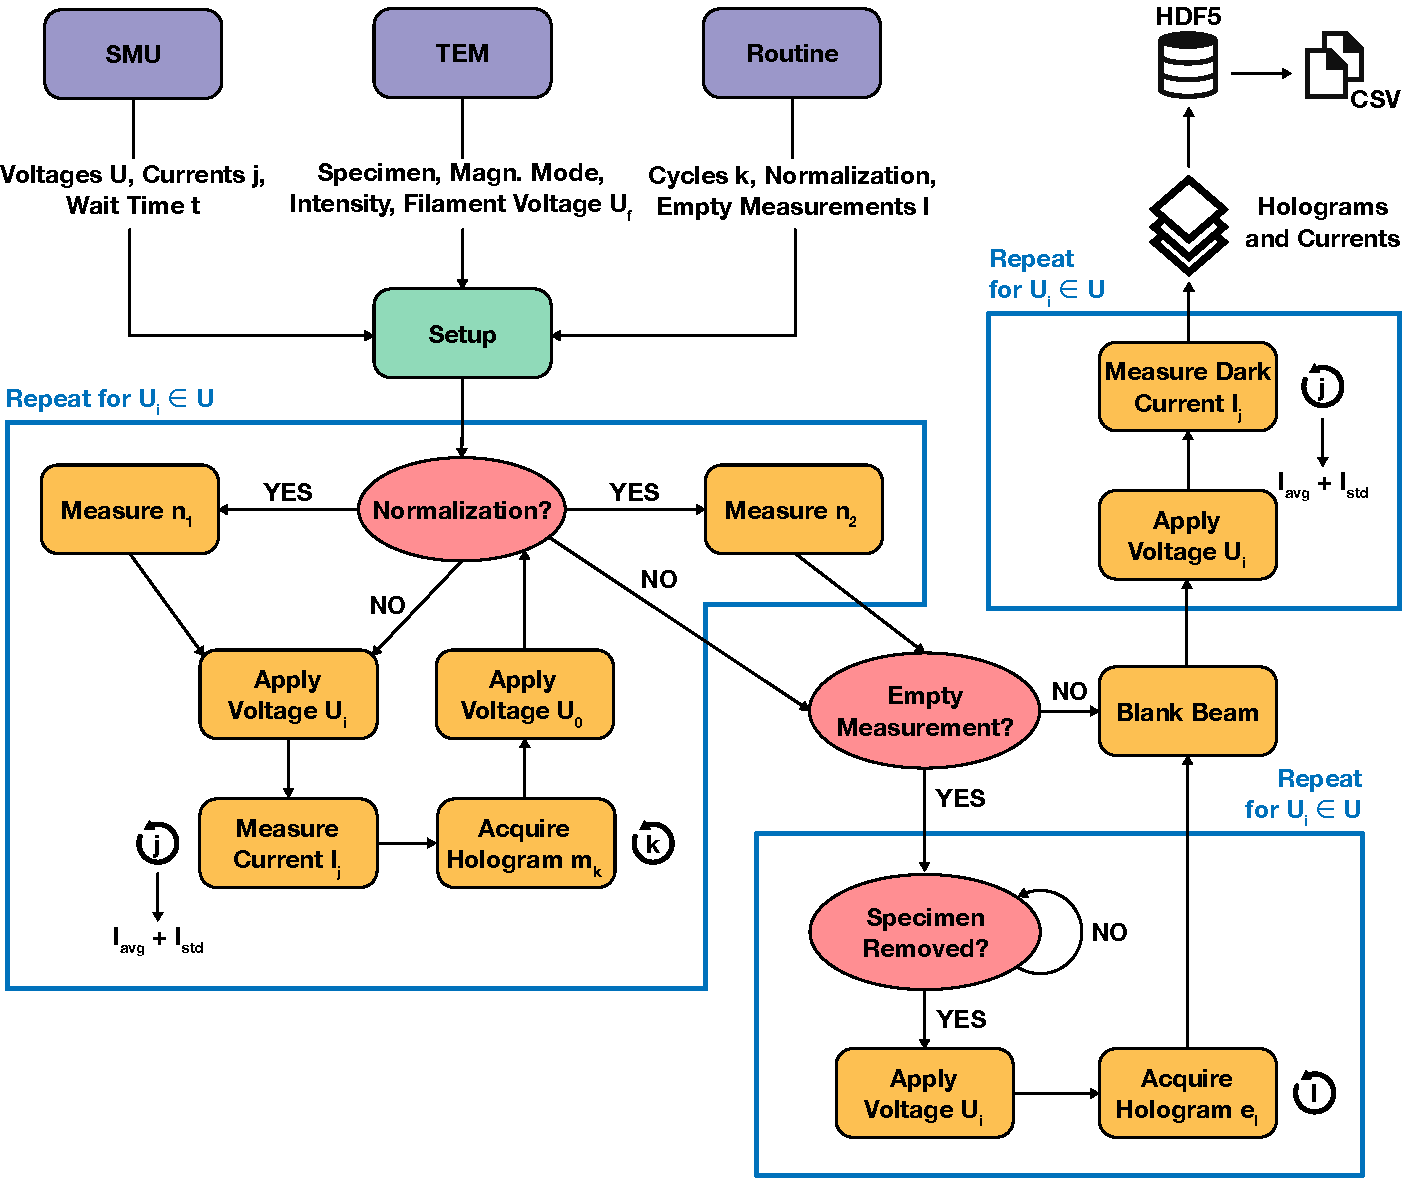
\includegraphics[width=\textwidth]{Figures/Schematics/Automation/flowchart-automatic-holography-measurement.pdf}
	\caption{Flowchart detailing the automated measurement process using the self-developed \emph{HoloSuite} software package: Extensive customization options regarding the various measurement parameters concerning the SMU, TEM and measurement routine allow for the fully automated acquisition of the electron holograms $m_k$, the normalization holograms $n_1$ and $n_2$, and the empty holograms $e_l$ for every applied bias voltage $U_i$, as well as the average (dark) currents $I_{\mathit{avg}}$ and corresponding standard deviation $I_{\mathit{std}}$.}
	\label{fig:flowchart-automatic-holography-measurement}
\end{figure}
In order to obtain the desired measurement data, \emph{HoloSuite} offers extensive customization options regarding the various measurement parameters found in a modern experimental setup. These parameters can be classified into three groups, depending on whether they concern the SMU, the TEM or the actual measurement routine. The parameters regarding the SMU specify the external biasing voltages $U_{\mathit{ext}}$ that are applied to the specimen, defined by a start and end voltage, along with the step size between them, the voltage and current range of the SMU, the number of currents $j$ that are measured for each applied voltage $U_i$ and subsequently averaged, and the wait time $t$ between the various changes of the SMU and the hologram acquisition. The second set of parameters concerns all settings regarding the TEM and is mostly used to properly name the resulting dataset, containing the name of the specimen, the magnification mode (i.\,e.\ SA or Lorentz mode), the C2~lens intensity, the filament voltage $U_f$ and the acceleration voltage $U_{\mathit{acc}}$, along with the exposure time $t_{\mathit{exp}}$ for each acquired hologram. The final set of parameters deals with the automated measurement routine itself and contains the number of holograms $k$ acquired per applied voltage $U_i$, whether to obtain two normalization holograms $n_1$ and $n_2$ and the number of empty holograms $l$ per applied voltage $U_i$.

With the all required parameters specified, \emph{HoloSuite} first connects to the SMU using a network socket and a specified IP~address and port. If the connection was successful, the output terminals of the SMU are turned on and the specified voltage and current ranges are applied (therefore disabling the default auto range option). The remote connection to the TEM is likewise established using the \emph{temscript} software package, a \textsc{python} wrapper for the TEMScripting interface by FEI™ \cite{temscript}, via a provided IP~address and port. After a successful connection to the TEM, the output dataset is allocated on the hard disk, where the filename is generated from the second set of parameters specified above. The dataset itself is written to and accessed by using the \emph{h5py} package, where the open HDF5 standard is optimized for storing and accessing large amounts of data and not only allows filesystem-like arbitrary organization into (sub-)groups, but also flexible metadata associated with every object \cite{Collette2014}.

The first series of measurements is acquired by looping over every external bias voltage, starting from the one with the smallest absolute value\footnote{Usually $U_{\mathit{ext}} = \SI{0}{\volt}$.} and increasing in an alternating pattern between forward and reverse bias\footnote{This is done in order to minimize the change of damaging the specimen by suddenly applying a large external bias voltage.}. For every voltage $U_i$, a corresponding group is created in the HDF5 dataset, with the applied voltage as its name. After which, if specified, the first normalization hologram $n_1$ of the unbiased specimen (i.\,e.\ $U_{\mathit{ext}} = \SI{0}{\volt}$), with the desired exposure time $t_{\mathit{exp}}$, is acquired. Afterwards, the current biasing voltage $U_i$ is applied via the SMU and the current is measured $j$ times, yielding the corresponding average current $I_{\mathit{avg}}$ and standard deviation $I_{\mathit{std}}$. Thereafter, the $k$ actual electron holograms $m_k$ are measured, each with an exposure time of $t_{\mathit{exp}}$. Upon applying a biasing voltage of $U_{\mathit{ext}} = \SI{0}{\volt}$ again, the second normalization hologram $n_2$ is acquired, if specified.

The second series of measurements contains all empty holograms, where $l$ empty holograms $e_l$ are acquired for every applied voltage $U_i$. Here, if needed, the user is given the opportunity to remove the specimen from the field of view and thus also from acquired holograms.
\newpage
Regardless of whether \emph{HoloSuite} is set to acquire empty holograms or not, the automated measurement always contains a series of dark currents. Here, the electron beam is first blanked, after which the current is measured $j$ times for every applied voltage $U_i$, resulting in the corresponding average dark current $I_{\mathit{avg}}$ and standard deviation $I_{\mathit{std}}$.

In addition to the HDF5 dataset, that not only contains all holograms but also the average (dark) currents $I_{\mathit{avg}}$ and corresponding standard deviations $I_{\mathit{std}}$, the $I$-$V$~curves are written as comma-separated values (CSV) to a text file. \emph{HoloSuite} therefore significantly cuts down on measurement time, reducing the required time (excluding TEM alignment) from a full work day to around 30~minutes or less, where the resulting HDF5 dataset ranges from a few hundred~MB to multiple~GB, depending on the specified voltage range and desired number of holograms. The automated measurement finishes by unblanking the electron beam, turning off the SMU outputs and closing the connecting network socket.
\subsection{Automated Reconstruction} \label{ssec:holosuite-automated-reconstruction}
In order to obtain the full set of information carried by the previously acquired electron
holograms, a two-step reconstruction process has to be carried out \cite{Voelkl1999,Lehmann2002,Lichte2008}. While improving the signal-to-noise ratio (SNR) can, in principle, be done by lengthened exposure times $t_{\mathit{exp}}$, a multitude of instrumental instabilities (especially in the high-resolution domain) make this approach, at least without sophisticated feedback control in the experimental setup \cite{Gatel2018,Takahashi2020}, practically unfeasible \cite{Niermann2014}. Using a special reconstruction algorithm featuring an advanced averaging scheme implemented in the \emph{holoaverage} software package proves to be a viable and suitable solution \cite{Niermann2014}, motivating the acquisition of multiple holograms per applied bias voltage $U_i$ in the automated measurement process of \emph{HoloSuite}.
\newpage
With the measurement dataset obtained by automated acquisition detailed in \cref{ssec:holosuite-automated-measurement}, the automated reconstruction and post-processing of electron holograms implemented in \emph{HoloSuite} can be divided into two parts (\cref{fig:flowchart-automatic-holography-post-processing}): While the first part deals with the actual reconstruction of the electron holograms using \emph{holoaverage}'s averaging scheme \cite{Niermann2014}, the second part obtains various physical quantities of the specimen, such as the phase modulation $\varphi$ and its first- and second-order derivative $\dv*{\varphi}{x}$ and $\dv*[2]{\varphi}{x}$ (which are proportional to the electric field $E$ and the charge carrier density $\rho$, respectively), through a multi-step post-processing method.
\begin{figure}[H]
	\centering
	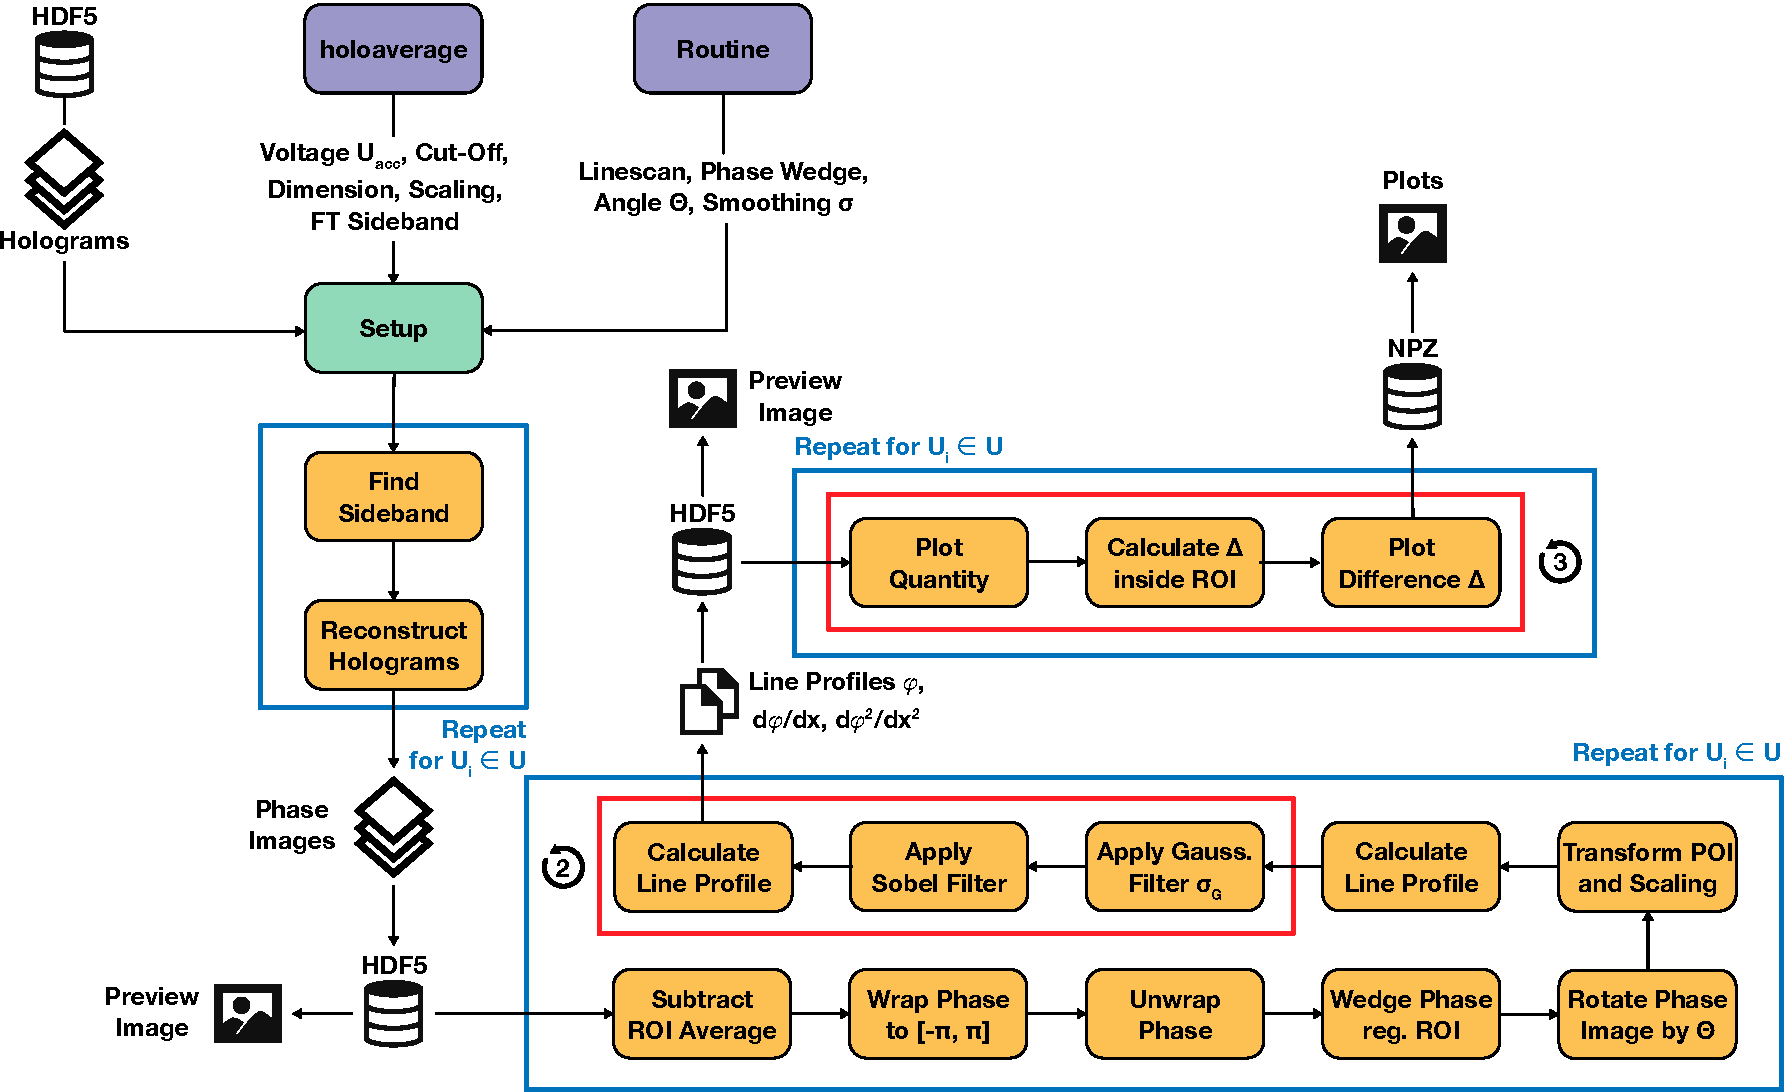
\includegraphics[width=\textwidth]{Figures/Schematics/Automation/flowchart-automatic-holography-post-processing.pdf}
	\caption{Flowchart detailing the automated reconstruction and post-processing method using the self-developed \emph{HoloSuite} software package: Initially, the previously acquired electron holograms are reconstructed using \emph{holoaverage}'s reconstruction algorithm \cite{Niermann2014}, followed by a multi-step post processing method to obtain various physical quantities of the specimen, such as the phase modulation $\varphi$ and its first- and second-order derivative $\dv*{\varphi}{x} \propto E$ and $\dv*[2]{\varphi}{x} \propto \rho$.}
	\label{fig:flowchart-automatic-holography-post-processing}
	\vspace*{-3mm}
\end{figure}
In line with the previously described automated measurement process, \emph{HoloSuite} offers extensive customization options regarding the actual electron hologram reconstruction as well as the post-processing routine. These parameters can again be classified into different groups, depending on whether they concern the electron hologram reconstruction using \emph{holoaverage} or the post-processing of these reconstructed holograms. The parameters regarding \emph{holoaverage} specify the acceleration voltage $U_{\mathit{acc}}$ used for acquisition, the cut-off frequency in Fourier space, the size of the reconstructed object hologram, the sampling factor and the quadrant of the sideband in Fourier space. The second set of parameters contains all the information needed for the post-processing of the reconstructed electron holograms, consisting of the line profile coordinates and width, the phase wedge position, width and number of times it is applied, the angle $\theta$ by which the electron holograms are rotated and the standard deviation $\sigma_G$ of the Gaussian kernel used for smoothing.

After all necessary parameters are specified, \emph{HoloSuite} begins with the reconstruction of the electron holograms through the supplied HDF5 dataset. For each applied bias voltage $U_i$, \emph{HoloSuite} automatically finds the pixel position of the sideband in Fourier space needed for reconstruction. This is done by cropping the electron holograms to the specified quadrant, on top of a (customize) cut-off around the edges\footnote{This additional cut-off around the edges of the isolated quadrant in Fourier space is done in order to ensure that the brightest pixel actually corresponds to the sideband and not the autocorrelation of the electron hologram.}, and finding the brightest pixel. After which, a (customizable) region of interest (ROI) around this pixel is isolated and a center of mass calculation is applied using the \emph{SciPy} software package \cite{Virtanen2020} (which is also used for the Fourier transform and the later image rotation, smoothing and derivative) to find the sub-pixel position of the sideband. This sub-pixel position of the sideband, along with all the above mentioned parameters, are passed to \emph{holoaverage}, yielding the (complex valued) averaged reconstructions of the normalized and drift aligned object holograms for every applied bias voltage $U_i$. In order to also obtain the phase images, the counterclockwise angles from the positive real axis on the complex plane are calculated using the \emph{NumPy} software package \cite{Harris2020} (which is also used for all general mathematical calculation, such as averaging, standard deviation and so forth). If specified, the two normalization measurements $n_1$ and $n_2$ are passed as pseudo-empty measurements to \emph{holoaverage} instead of the acquired holograms $e_l$.

After all acquired measurements have been reconstructed, \emph{HoloSuite} outputs all electron holograms and phase images to a HDF5 dataset, where each group corresponds to the applied bias voltage $U_i$ and contains two 2D~datasets with the above specified output dimension, along with one preview phase image (for a customizable bias voltage) as a TIFF file. In addition, all metadata provided by \emph{holoaverage}, such as the scaling factor of the reconstructed electron holograms and the spatial frequency of the reconstructed sideband, is copied over and written as attributes to the HDF5 output file for each dataset.

With the reconstruction completed, the phase images have to be post-processed using a comprehensive workflow. For this, \emph{HoloSuite} starts by looping over every phase image in the provided HDF5 dataset and subtracting the average of the phase wedge ROI (i.\, e. offsetting them so that they are close to zero within the phase wedge ROI). Since this leads to the phase images no longer being constrained to an interval of $\interval{-\pi}{\pi}$, they are again wrapped back to $\interval{-\pi}{\pi}$:
\begin{equation}
\vb*{\varphi}_{2\pi} = \arg\left(e^{i \cdot \vb*{\varphi}_{\mathit{off}}}\right),
\end{equation}
where $\vb*{\varphi}_{2\pi}$ represents the $\interval{-\pi}{\pi}$ wrapped phase image, $\vb*{\varphi}_{\mathit{off}}$ the non-constrained phase image obtained through the subtraction of the phase wedge ROI and $\arg$ the angle of the complex argument. This phase wrapping to $\interval{-\pi}{\pi}$ is done to ensure that the subsequent phase unwrapping using \emph{scikit-image}'s implementation \cite{Vanderwalt2014} of a fast 2D~and 3D~algorithm based on sorting by reliability following a non-continuous path \cite{Herraez2002,AbdulRahman2005} produces reliable results. After unwrapping, the average of the phase wedge ROI is again subtracted from the phase images. Next, the phase images are modulated using a self-developed phase wedge method, where for every row inside the phase wedge ROI, a linear fit is calculated. These multiple linear fits are then averaged, and this average linear fit is extrapolated to all rows of the phase image and subsequently subtracted. This procedure is then repeated for every column, resulting in the wedged phase image:
\begin{gather}
\vb*{\varphi}_w = \vb*{\varphi}_{\gamma} - \overline{\mathcal{X}}_R\left(\vb*{\varphi}_{\gamma}\right) - \overline{\mathcal{X}}_C\left(\vb*{\varphi}_{\gamma}\right), \label{eq:holosuite-phase-wedge} \\
\overline{\mathcal{X}}_R = \sum\limits_{a=1}^{p \in \mathbb{N}} \frac{\mathcal{X}\left(\vb*{\varphi}_{\gamma}^a\right)}{p} \quad ; \quad \overline{\mathcal{X}}_C = \sum\limits_{b=1}^{p \in \mathbb{N}} \frac{\mathcal{X}\left(\vb*{\varphi}_{\gamma}^b\right)}{p}, \label{eq:holosuite-phase-wedge-average-fit}
\end{gather}
with the wedged phase image $\vb*{\varphi}_w$, the unwrapped and phase wedge ROI average subtracted phase image $\vb*{\varphi}_{\gamma}$, the linear fit $\mathcal{X}$ applied to every row $a$ and column $b$ across the phase wedge width $p$ (with $a, b, p \in \mathbb{N}$), and the averaged linear fits $\overline{\mathcal{X}}_R$ and $\overline{\mathcal{X}}_C$. Since the averaged linear fits inside the phase wedge ROI are sometimes not sufficiently flat enough after one calculation, the phase wedge is applied multiple times, where the number of repetitions is customizable.

Next, the phase images are rotated by the specified angle $\theta$, where $\theta$ is chosen such that the $p$-$n$-junction is orthogonal to the $x$-axis. Rotating an image by $\theta \in \left\{n \cdot \pi / 2 \, \middle| \, n \in \mathbb{N}\right\}$ yields an output image of equal shape. If, however, the angle is chosen such that $\theta \in \mathbb{R} \setminus \left\{n \cdot \pi / 2 \, \middle| \, n \in \mathbb{N}\right\}$, the output image has to either be cropped (if the same shape as the input image is desired, therefore losing information) or reshaped (if the input image is to be completely contained within output image, therefore increasing the image's shape through interpolation). Here, the output image is reshaped, meaning that all spatially dependent parameters, such as the line profile position, the phase wedge position or the scaling factor, have to be recalculated through a transformation from the input image to the output image.

Following the rotation of the phase images and the transformation of all points of interests, the first set of line profiles is calculated using \emph{scikit-image} at the specified start and end point. For every phase image, the line profile is reduced across the specified line profile width from a 2D~rectangle to 1D~curve, where the aggregation of pixel values perpendicular to the line profile is calculated through averaging. This 1D line profile returns the phases $\varphi$ (i.\,e.\ the projected electrostatic potentials $\phi$) for every applied bias voltage $U_i$. In order to obtain a quantity proportional to the electric fields $E$ across the same line profile region, the first-order derivative in $x$-direction for all phase images is calculated. This is done through the convolution with a Sobel filter, where all phase images are smoothed beforehand using a 2D~Gaussian filter and the specified $\sigma_G$. After which, the same 1D line profile can be calculated, yielding $\dv*{\varphi}{x} \propto E$. A second subsequent and identical smoothing and second-order derivative is applied, from which, with the use of the aforementioned line profile, a quantity proportional to the charge carrier density $\rho$ can be calculated, resulting in $\dv*[2]{\varphi}{x} \propto \rho$. As with the automatic reconstruction using \emph{holoaverage}, a preview PNG image is saved for a customizable external bias voltage, with the phase wedge ROI and line profile area indicated by differently colored rectangles.

One of the advantages of the automated acquisition of large datasets is the ability to investigate the changes in the various physical properties of the specimen caused by applying an external bias voltage. Of particularly great interest is the change in the phase, and thus the first- and second-order derivative, when an external bias voltage is applied in both forward and reverse direction, compared to the case where no external bias voltage is applied. For the three above mentioned physical properties $\varphi$, $\dv*{\varphi}{x}$ and $\dv*[2]{\varphi}{x}$, this is done by:
\begin{itemize}
	\item \textbf{Phase $\varphi$}: Find the $\SI{10}{\percent}$ interval with the highest average value in a range of $\SIrange{40}{80}{\percent}$ and subtract if from the closest average to zero in a range of $\SIrange{10}{40}{\percent}$;
	\item \textbf{First-Order Derivative $\dv*{\varphi}{x} \propto E$}: Find the $\SI{10}{\percent}$ interval with the lowest average value in a range of $\SIrange{20}{80}{\percent}$ and subtract if from the closest average to zero in a range of $\SIrange{10}{40}{\percent}$;
	\item \textbf{Second-Order Derivative $\dv*[2]{\varphi}{x} \propto \rho$}: Find the $\SI{10}{\percent}$ interval with the lowest or highest average value in a range of $\SIrange{20}{80}{\percent}$ and subtract if from the closest average to zero in a range of $\SIrange{10}{40}{\percent}$ or $\SIrange{60}{90}{\percent}$, respectively.
\end{itemize}
The average values for this computation are calculated by taking a moving average equal in size to approximately $\SI{10}{\percent}$ of the whole 1D~line profile, where the step size is one data point. By not searching the entire 1D~line profile for the highest/lowest average interval, but omitting at least approximately $\SI{10}{\percent}$ of the line profile at both ends, ensures that outliers caused e.\,g.\ by boundary effects at the contacts have no influence on the automatic post-processing. For all calculated data points $\Delta \varphi$, $\Delta \dv*{\varphi}{x}$ and $\Delta \dv*[2]{\varphi}{x}$, the measurement uncertainty is given by the standard deviation of the corresponding $\SI{10}{\percent}$ interval.

After processing all 1D~line profiles and their changes for different externally applied bias voltages, they are plotted using the \emph{matplotlib} software package \cite{Hunter2007}. Furthermore, the post-processed phase images, along with their first- and second-order derivatives, are stored in an additional HDF5 dataset, along with their respective 1D~line profiles. These 1D~line profiles and their changes for different externally applied bias voltages, which are in the form of binary \emph{NumPy} arrays (i.\,e.\ \texttt{.npy}), are further stored in an uncompressed container format (i.\,e.\ \texttt{.npz}) for easier post-processing.

\chapter{Results} \label{chap:experimental-results}
Using the automated measurement and post-processing workflow for off-axis EH detailed in \cref{ssec:off-axis-EH-experimental-setup} as well as FEM simulations using the \emph{ONELAB} and \emph{nextnano} software packages described in \cref{sec:numerical-modeling}, the following chapter details the results obtained from both experimental measurements and simulations and compares them in the context of quantitative agreement.
\section{Coplanar Capacitor} \label{sec:experimental-results-coplanar-capacitor}
The ubiquitous coplanar capacitor, whose preparation is described in detail in \cref{ssec:specimen-preparation-capacitor}, was used as a reference specimen due to its well known geometry and electrostatic behavior.
\subsection{Off-Axis Electron Holography} \label{ssec:experimental-results-capacitor-EH}
For the first measurement series, three object holograms and two empty holograms were recorded for an exposure time of $T_{\mathit{exp}} = \SI{5}{\second}$ each using a filament voltage of $U_f \approx \SI{75}{\volt}$. The external electrical bias $U_{\mathit{ext}}$ was chosen from $\SIrange{-1.5}{1.5}{\volt}$ in increments of $\SI{0.3}{\volt}$ as well as $\SIrange{-1.0}{1.0}{\volt}$ in increments of $\SI{0.5}{\volt}$. The acquired holograms were then reconstructed using the upper sideband where a 14\textsuperscript{th} degree Butterworth filter with a cut-off frequency of $1/\SI[per-mode=power]{11.4}{\per\nm}$, yielding a spatial resolution of approximately $\SI{20}{\nm}$ \cite{Lehmann2002,Lichte2008}, was applied.
\newpage
For an external bias voltage of $U_{\mathit{ext}} = \SI{1}{\volt}$ applied to the upper contact, with the lower contact grounded, the reconstructed amplitude $A$ (normalized to $1$) and its line profile $A\left(x\right)$ (illustrated by a blue rectangle with an arrow indicating the direction) show a constant behavior between the capacitor plates with slight modulations at the edges due to Fresnel fringes (\cref{fig:capacitor-off-axis-EH-linescans}a). The reconstructed phase $\varphi$ on the other hand is constrained to an interval of $\interval{-\pi}{\pi}$, where its line profile $\varphi\left(x\right)$ in the same region as \cref{fig:capacitor-off-axis-EH-linescans}a) shows a linear trend between the capacitor plates and noise within them (\cref{fig:capacitor-off-axis-EH-linescans}b).
\begin{figure}[H]
	\centering
	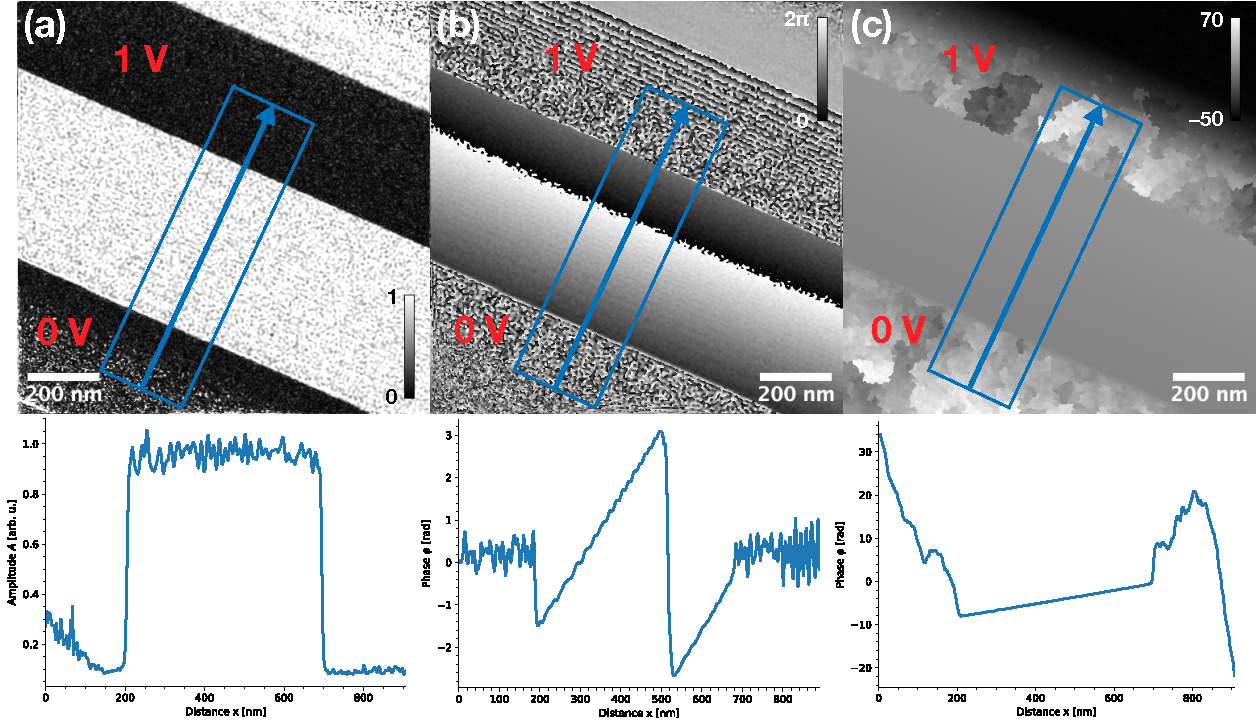
\includegraphics[width=\textwidth]{Figures/Results/Capacitor/Holography/capacitor-off-axis-EH-linescans.pdf}
	\caption{Electron holography for a coplanar capacitor biased with $U_{\mathit{ext}} = \SI{1}{\volt}$ with (a) the reconstructed amplitude and its corresponding line profile $A\left(x\right)$, (b) the reconstructed phase and its corresponding $2\pi$-wrapped line profile $\varphi\left(x\right)$ and (c) the same reconstructed phase and its line profile unwrapped.}
	\label{fig:capacitor-off-axis-EH-linescans}
\end{figure}
Unwrapping the phase image yields the same linear trend with the $2\pi$ phase jumps removed (\cref{fig:capacitor-off-axis-EH-linescans}c), while the unwrapping algorithm produces undefined behavior for the contacts consisting primarily of noise and arbitrary phase offsets for non-contiguous areas (e.\,g.\ reference window).
\newpage
Comparing the phase image for an applied external bias of $U_{\mathit{ext}} = \SI{1}{\volt}$ with the phase image for a short-circuited setup (i.\,e.\ $U_{\mathit{ext}} = \SI{0}{\volt}$), the vacuum region between the electrodes exhibits a characteristic gradient perpendicular to the surfaces of the capacitor plates (\cref{fig:capacitor-off-axis-EH-slope}a). Furthermore, varying the applied external bias between $U_{\mathit{ext}} = \SI{-1.5}{\volt}$ and $U_{\mathit{ext}} = \SI{1.5}{\volt}$ and normalizing the phase slopes $\dv*{\varphi}{x}$ calculated inside the vacuum region (illustrated by a blue rectangle with an arrow indicating the direction) to the phase slope at $U_{\mathit{ext}} = \SI{0}{\volt}$ displays the expected linear proportionality between the phase (and therefore the electrostatic potential) and the applied external voltage (\cref{fig:capacitor-off-axis-EH-slope}b).
\begin{figure}[H]
	\centering
	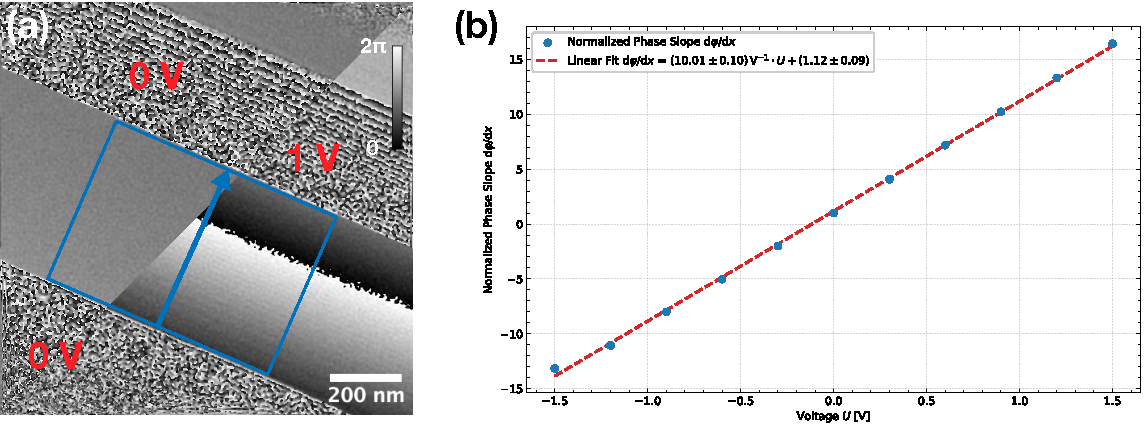
\includegraphics[width=\textwidth]{Figures/Results/Capacitor/Holography/capacitor-off-axis-EH-slope.pdf}
	\caption{Electron holography for a coplanar capacitor (a) biased with $U_{\mathit{ext}} = \SI{0}{\volt}$ and $U_{\mathit{ext}} = \SI{1}{\volt}$ and (b) the phase slopes $\dv*{\varphi}{x}$ for different external biasing voltages normalized to the phase slope at $U_{\mathit{ext}} = \SI{0}{\volt}$.}
	\label{fig:capacitor-off-axis-EH-slope}
\end{figure}
These observations not only illustrate the excepted linear slope of the electrostatic potential inside a vacuum region between two capacitor plates, which is linearly proportional to the applied external bias, but also show that EH is a suitable technique for the measurement of pure phase objects (as is the case here) where there is no apparent amplitude modulation.
\newpage
\subsection{Finite Element Method Simulation} \label{ssec:experimental-results-capacitor-FEM-simulation}
A comparable coplanar capacitor is modeled using the \emph{ONELAB} software package (\cref{fig:capacitor-FEM-EH-linescan-comparison}), whose exact geometric layout (\cref{fig:specimen-capacitor-layout}) is described in detail in \cref{ssec:2d-modeling-specimen}.
\begin{figure}[H]
	\centering
	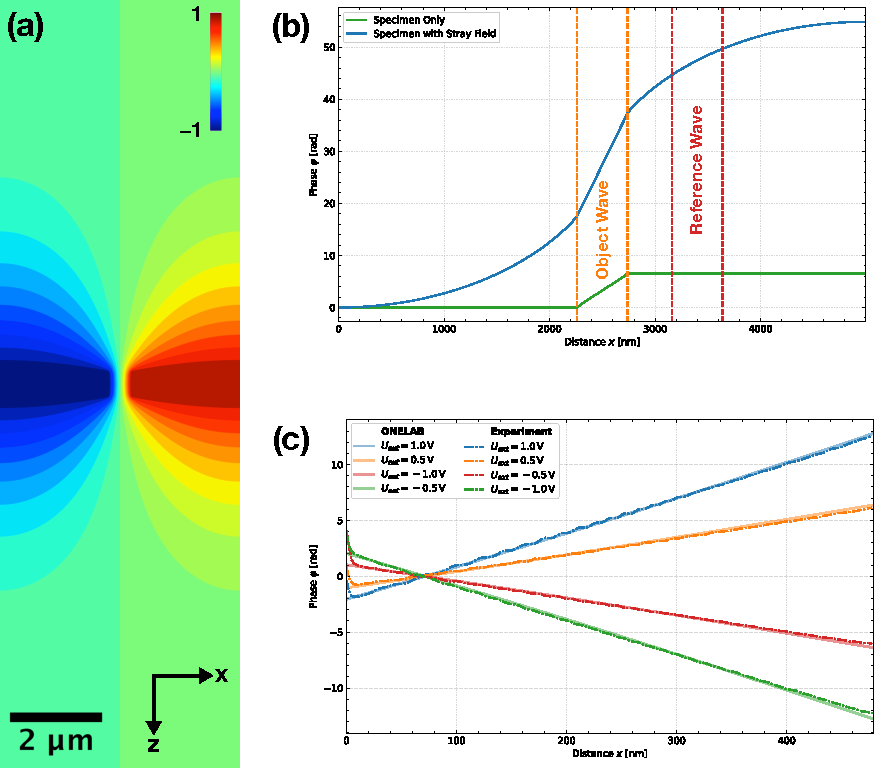
\includegraphics[width=\textwidth]{Figures/Results/Capacitor/Simulations/capacitor-FEM-EH-linescan-comparison.pdf}
	\caption{FEM simulation of the coplanar capacitor biased with $U_{\mathit{ext}} = \SI{1}{\volt}$ where (a) the 2D~electrostatic potential $\phi$ yields (b) the phase $\varphi$ through projection, (c) which is compared with the above detailed experimentally acquired holograms for different applied bias voltages.}
	\label{fig:capacitor-FEM-EH-linescan-comparison}
\end{figure}
The 2D~electrostatic potential $\phi$ obtained through this method shows that, while the contacts exhibit a constant potential of $\pm U_{\mathit{ext}}$, respectively, the stray field extents deep into the vacuum region above and below the capacitor, only approaching zero after several $\si{\um}$ (\cref{fig:capacitor-FEM-EH-linescan-comparison}a). This behavior is especially apparent when calculating the phase $\varphi$ through a projection (without any weighting applied to the different specimen regions), where the specimen (i.\,e.\ the capacitor itself) only contributes a small parts to the overall phase (approximately 8\% of the maximum phase shift), which is predominantly made up of the stray field contribution (\cref{fig:capacitor-FEM-EH-linescan-comparison}b, with both phases offset to zero through subtraction by the first value). Additionally, by defining the object wave $\varphi_{\mathit{obj}}$ to correspond to the vacuum region between the contacts (\cref{fig:capacitor-FEM-EH-linescan-comparison}b, indicated by the dashed orange lines) and the reference wave $\varphi_{\mathit{ref}}$ to a region of the same size offset $\SI{800}{\nm}$ to the right (\cref{fig:capacitor-FEM-EH-linescan-comparison}b, indicated by the dashed red lines), comparisons to the above experimentally acquired phases are made (\cref{fig:capacitor-FEM-EH-linescan-comparison}c).

Here, it is evident that for all external bias voltages $U_{\mathit{ext}}$, ranging from $\SIrange{-1.0}{1.0}{\volt}$ in increments of $\SI{0.5}{\volt}$, the simulated phases are in excellent agreement with the experimental phases acquired through off-axis EH.\footnote{Since the simulated coplanar capacitor was electrically biased by applying $\pm U_{\mathit{ext}}$ at the contacts, while the experimentally measured capacitor was grounded at one of the contacts, a scaling factor of $2$ has been applied when calculating the phase through projection.}

Through the comparison with 2D~simulations of the electrostatic potential, it is evident that FEM simulations are in excellent agreement with real-world measurements and are able to reliably describe the behavior of simple specimens. Furthermore, by separating the projected electrostatic potential into a specimen and stray field region, it is apparent that the specimen region of the coplanar capacitor only contributes a small part to the overall phase, necessitating a model which takes these effects into account.
\section[\texorpdfstring{$p$-$p^+$-$n^+$}{\textit{p}-\textit{p}\textsuperscript{+}-\textit{n}\textsuperscript{+}}-Junction]{$\boldsymbol{p}$-$\boldsymbol{p^+}$-$\boldsymbol{n^+}$-Junction}
The previous \cref{sec:experimental-results-coplanar-capacitor} successfully demonstrated the reliability of off-axis EH by analyzing the electrostatic behavior exhibited by a coplanar capacitor, which served as a well-understood reference specimen. This section shifts the focus towards the investigation of real semiconductor nanostructures, where a $p$-$p^+$-$n^+$-junction, whose preparation is described in detail in \cref{ssec:specimen-preparation-pn-junction}, serves as an exemplary specimen.
\subsection{Off-Axis Electron Holography} \label{ssec:experimental-results-ppn-junction-off-axis-EH}
The measurement series for the $p$-$p^+$-$n^+$-junction consisted of three object holograms and two empty holograms with an exposure time of $T_{\mathit{exp}} = \SI{5}{\second}$ each. The filament voltage was set to $U_f \approx \SI{69}{\volt}$ and the external electrical bias $U_{\mathit{ext}}$ was chosen from $\SIrange{0.0}{3.0}{\volt}$ in increments of $\SI{0.5}{\volt}$. Similar to the above described coplanar capacitor, the acquired holograms were reconstructed by applying a 14\textsuperscript{th} degree Butterworth filter with a cut-off frequency of $1/\SI[per-mode=power]{11.4}{\per\nm}$, whereas in this case the lower sideband was used.
\newpage
The diode was contacted with an external bias $U_{\mathit{ext}}$ at the $n^+$-doped region, whereas the $p$-doped region was grounded. By applying an external bias of $U_{\mathit{ext}} = \SI{2}{\volt}$ (i.\,e.\ reverse bias), the reconstructed amplitude $A$ exhibits a constant line profile $A\left(x\right)$ (illustrated by a blue rectangle with an arrow indicating the direction) across the junction (\cref{fig:pn-junction-off-axis-EH-linescans}a), similar to the above described coplanar capacitor. As is the case with the coplanar capacitor, the reconstructed phase $\varphi$ (with a phase wedge applied in the $p$-doped region) is constrained to an interval of $\interval{-\pi}{\pi}$, with its line profile $\varphi\left(x\right)$ displaying a characteristic phase jump caused by the built up of a potential barrier at the depletion region (\cref{fig:pn-junction-off-axis-EH-linescans}b).
\begin{figure}[H]
	\centering
	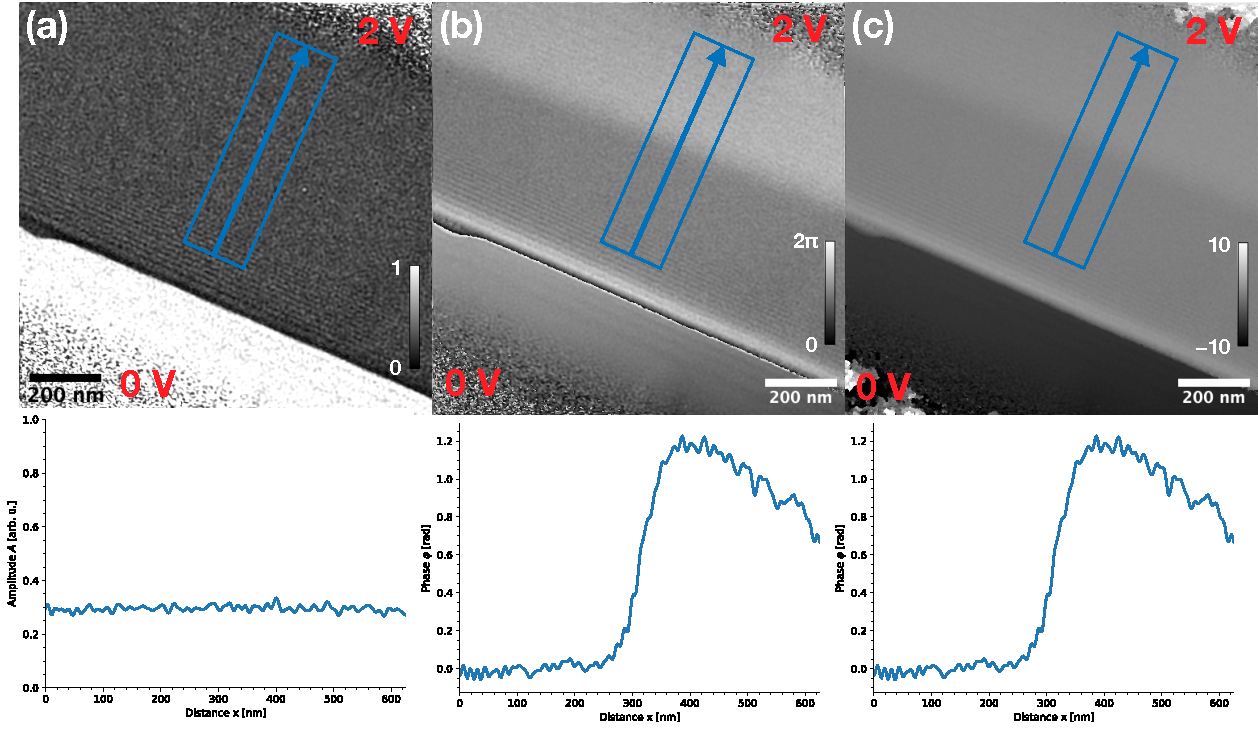
\includegraphics[width=\textwidth]{Figures/Results/pn-Junction/Holography/pn-junction-off-axis-EH-linescans.pdf}
	\caption{Electron holography for a $p$-$p^+$-$n^+$-junction reverse biased with $U_{\mathit{ext}} = \SI{2}{\volt}$ with (a) the reconstructed amplitude and its corresponding line profile $A\left(x\right)$, (b) the reconstructed phase (with a phase wedge applied in the $p$-doped region) and its corresponding $2\pi$-wrapped line profile $\varphi\left(x\right)$ and (c) the same reconstructed phase and its line profile unwrapped.}
	\label{fig:pn-junction-off-axis-EH-linescans}
\end{figure}
Unwrapping the phase image reveals an identical line profile across the junction due to the measured phase jump being smaller than $2\pi$ (\cref{fig:pn-junction-off-axis-EH-linescans}c), while unwrapping algorithm once again produces undefined behavior towards the contacts of the specimen.
\newpage
By comparing the phases images for an applied external bias of $U_{\mathit{ext}} = \SI{0}{\volt}$ and $U_{\mathit{ext}} = \SI{3}{\volt}$, only a moderate difference in the phase jump in reverse bias condition is observed (i.\,e.\ smaller than $2\pi$), indicating an abnormal switching behavior (\cref{fig:pn-junction-off-axis-EH-phase-jump}a). By comparing the phase jumps $\Delta \varphi\left(x\right)$ across the junction (illustrated by a blue rectangle with an arrow indicating the direction) for the different external bias voltages (after unwrapping and modulating each phase image by a phase wedge), the phase jumps, nonetheless, qualitatively demonstrate the expected proportionality to the externally applied voltage (\cref{fig:pn-junction-off-axis-EH-phase-jump}b).
\begin{figure}[H]
	\centering
	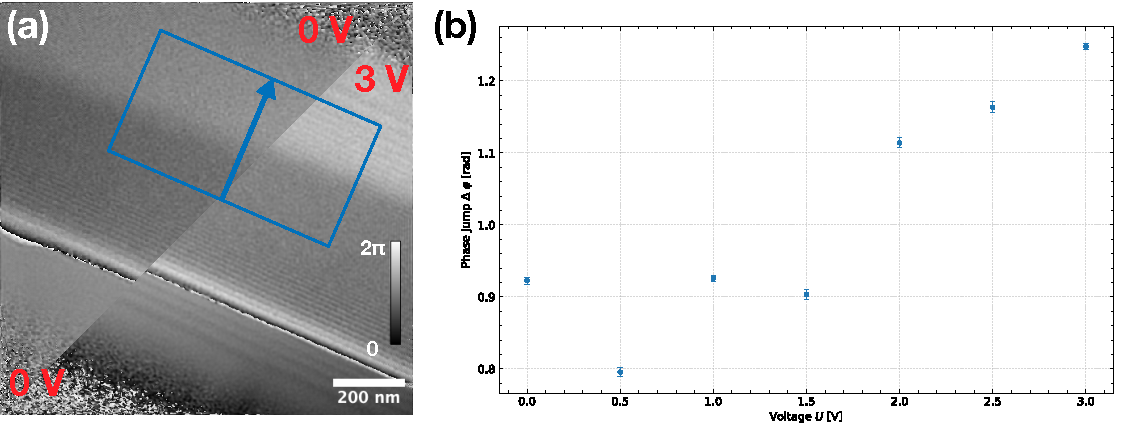
\includegraphics[width=\textwidth]{Figures/Results/pn-Junction/Holography/pn-junction-off-axis-EH-phase-jump.pdf}
	\caption{Electron holography for a $p$-$p^+$-$n^+$-junction (a) $U_{\mathit{ext}} = \SI{0}{\volt}$ and $U_{\mathit{ext}} = \SI{3}{\volt}$ at the $n^+$-doped region and grounded (i.\,e.\ $U_{\mathit{ext}} = \SI{0}{\volt}$) at the $p$-doped region and (b) the phase jumps $\Delta \varphi\left(x\right)$ for different external biasing voltages.}
	\label{fig:pn-junction-off-axis-EH-phase-jump}
\end{figure}
These observations, through the investigation of the proportionality of the phase jumps to the applied external bias, once again demonstrate the robustness of off-axis EH as a measurement technique suitable for different kinds of specimen.
\newpage
\subsection{Finite Element Method Simulation} \label{ssec:experimental-results-pnjunction-FEM-simulation}
Similar to \cref{ssec:experimental-results-capacitor-FEM-simulation}, a comparable $p$-$p^+$-$n^+$-junction is modeled using the \emph{nextnano} software package (\cref{fig:pn-junction-FEM-EH-linescan-comparison}), whose exact geometric layout (\cref{fig:specimen-nextnano-layout}) is described in detail in \cref{ssec:2d-modeling-specimen}.
\begin{figure}[H]
	\centering
	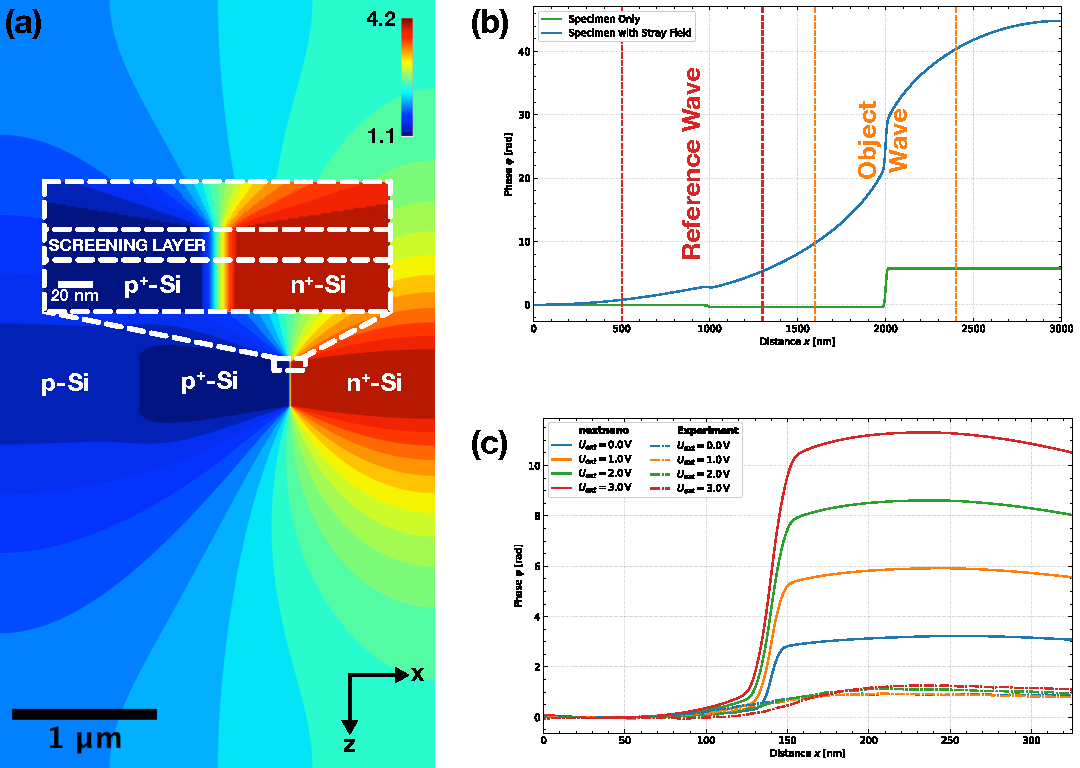
\includegraphics[width=\textwidth]{Figures/Results/pn-Junction/Simulations/pn-junction-FEM-EH-linescan-comparison.pdf}
	\caption{FEM simulation of the $p$-$p^+$-$n^+$-junction reverse biased with $U_{\mathit{ext}} = \SI{2}{\volt}$ where (a) the 2D~electrostatic potential $\phi$ yields (b) the phase $\varphi$ through projection, (c) which is compared with the above detailed experimentally acquired holograms for different applied bias voltages.}
	\label{fig:pn-junction-FEM-EH-linescan-comparison}
\end{figure}
The 2D~electrostatic potential $\phi$ obtained through this method shows, similar to the above described coplanar capacitor, that, while the contacts exhibit a constant potential in $z$-direction in agreement with the expected behavior for a reverse biased diode, the stray field extents deep into the vacuum above and below the diode\footnote{By default, \emph{nextnano} assumes von~Neumann boundary conditions.} (\cref{fig:pn-junction-FEM-EH-linescan-comparison}a). Calculating the phase $\varphi$ through a projection of the electrostatic potential (without any weighting applied to the different specimen regions), where the specimen (i.\,e.\ the region inside the doped diode) once again only contributes a small parts to the overall phase (approximately 12\% of the maximum phase shift), which is predominantly made up of the stray field contribution (\cref{fig:pn-junction-FEM-EH-linescan-comparison}b, with both phases offset to zero through subtraction by the first value). Furthermore, by centering the object wave $\varphi_{\mathit{obj}}$ around the depletion region at the $p^+$-$n^+$-interface (\cref{fig:pn-junction-FEM-EH-linescan-comparison}b, indicated by the dashed orange lines) and the reference wave $\varphi_{\mathit{ref}}$\footnote{According to \cref{ssec:FEM-simulated-potential-and-phase}, only the stray field contribution is considered for the reference wave (\cref{fig:flowchart-automatic-nextnano-post-processing}).} around a region of equal size offset $\SI{300}{\nm}$ to the left (\cref{fig:pn-junction-FEM-EH-linescan-comparison}b, indicated by the dashed red lines), comparisons to the above experimentally acquired phases are made (\cref{fig:pn-junction-FEM-EH-linescan-comparison}c).

For every externally applied reverse bias $U_{\mathit{ext}}$ ranging from $\SIrange{0.0}{3.0}{\volt}$, the simulated phases were an order of magnitude larger their phase jump and an order of magnitude smaller in their depletion region width, indicating large deviations between them. Even when taking into account the significantly smaller phase jumps, the experimentally acquired holograms do not exhibit the linear proportionality between the phase jumps and the externally applied bias voltage, suggesting an abnormal switching behavior caused by improper contacting.

The screening layer at the surface of the diode, whose thickness is characterized by the Debye length $\lambda_D$, has a negligibly small contribution to the overall phase, where $\lambda_D = \SI{18 \pm 5}{\nm}$ (\cref{fig:pn-junction-FEM-EH-linescan-comparison}a) is in the expected range for a sheet-like specimen \cite{Gurugubelli2015}. It is also worth noting that \emph{nextnano} only calculates the electrostatic potential $\phi_{\mathit{pn}}$ without considering the mean inner potential $\phi_{\mathit{MIP}}$ (\cref{eq:EH-phase-shift-specimen}), whose contribution, however, does not need to be taken into account due to the $p^+$-$n^+$-junction being a homojunction (i.\,e. $\phi_{\mathit{MIP}}$ would only add a constant phase shift).

Here, the experimentally acquired 2D~phase images were likewise modulated through the subtraction of a phase wedge (\cref{eq:holosuite-phase-wedge,eq:holosuite-phase-wedge-average-fit}), whereas the simulated phases were modulated through the subtraction of a linear fit, ranging from 10\% to 20\% and extrapolated to the entire field of view, from all values (\cref{ssec:FEM-simulated-potential-and-phase}).
\newpage
The above detailed simulations represent the electrostatic potential of a specimen that has suffered no sub-surface preparation damage. Even when accounting for the spatially widely extended stray field, which extends several $\si{\um}$ deep into the vacuum above and below the specimen, the simulated phases fail to accurately represent the experimentally obtained results, deviating by an order of magnitude in both the maximum phase shift and the depletion region width.

These observations suggest the existence of an electrically damaged crystalline layer (below the electrically inactive surface layer) resulting from Ga-induced defects during the FIB preparation stage (\cref{fig:FIB-preparation-damage-layer}), which is in agreement with previous results \cite{Twitchett2002,Beleggia2003,Cooper2006,Cooper2007,Twitchett-Harrison2007,Cooper2009,Somodi2013,Yazdi2015}.
\begin{figure}[H]
	\centering
	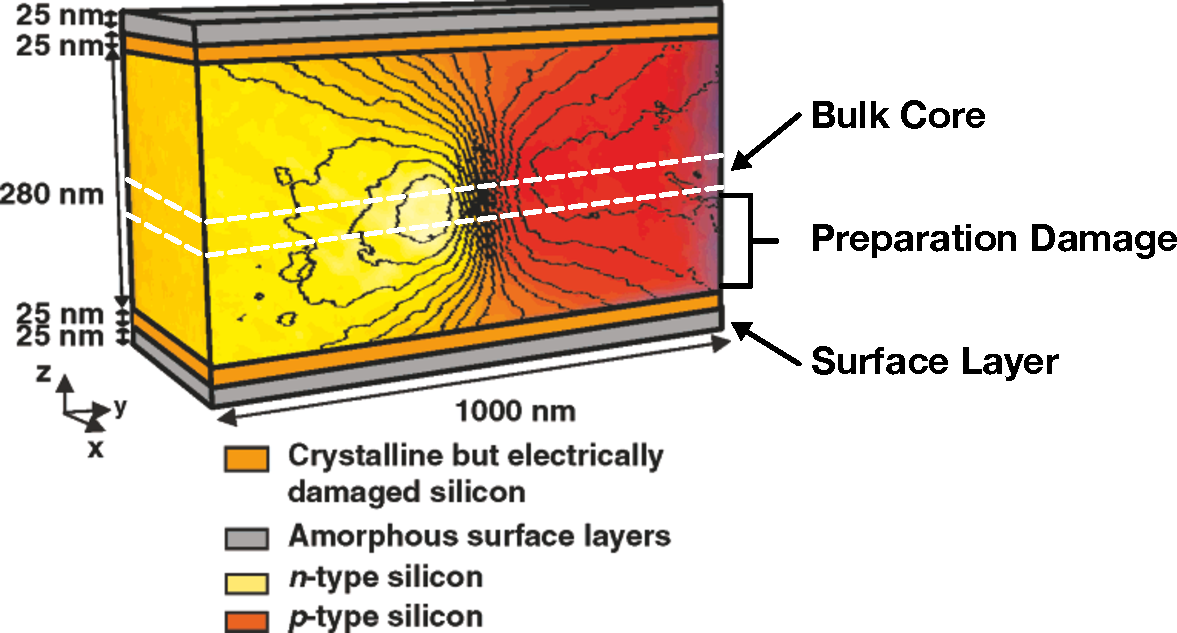
\includegraphics[width=\textwidth]{Figures/Schematics/FIB-preparation-damage-layer.pdf}
	\caption{3D~electrostatic potential obtained from the tomographic reconstruction of an electrically biased $p$-$n$-junction. Ga-induced defects caused by the FIB preparation of the specimen result in an electrically damaged crystalline layer below the electrically inactive surface layer (adapted from \cite{Twitchett-Harrison2007}).}
	\label{fig:FIB-preparation-damage-layer}
\end{figure}
Since the description of such damage effects with conventional FEM software packages proves to be impractical (as the exact distribution of the defects cannot be known), an alternative model, capable of accurately describing such real-world preparation defects (ideally with minimal prior knowledge of the specimen), is needed.

\chapter{Simple Intuitive Model for Potentials} \label{chap:SIMP}
The following chapter introduces a simple intuitive model for potentials (\emph{SIMP}) for both the coplanar capacitor and the $p$-$n$-junction, as well as its comparison with FEM simulations and experimental results obtained through off-axis electron holography and tomography.
\section{Mathematical Foundations}
Most software packages use some form of FEM (utilizing a mesh-based approach) for solving the Poisson (partial differential) equation, making such simulations computationally complex. The following \cref{ssec:classical-electrostatics} gives a brief insight into the Poisson equation and its solution using Green's function, while \cref{ssec:SIMP-alternative-model} derives an alternative model for the description of such electrostatic potentials in complex real-world specimens.
\subsection{Classical Electrostatics} \label{ssec:classical-electrostatics}
One of the foundations of electrostatics involves solving the Poisson equation:
\begin{equation}
  \laplacian \phi \left(\vb{r}\right) = -\frac{\rho\left(\vb{r}\right)}{\epsilon_0}
\end{equation}
for a given charge carrier density $\rho\left(\vb{r}\right)$ \cite{Jackson1999}. The solution for the scalar electrostatic potential is therefore given by:
\begin{equation}
  \phi \left(\vb{r}\right) = \frac{1}{4\pi \epsilon_0} \int \frac{\rho\left(\vb{r'}\right)}{\lvert \vb{r} - \vb{r'}\rvert} \dd{\vb{r'}} = \frac{1}{4\pi \epsilon_0} \int \rho\left(\vb{r'}\right) G_0\left(\vb{r}, \vb{r'}\right) \dd{\vb{r'}},
\end{equation}
where $G_0\left(\vb{r}, \vb{r'}\right) = \lvert \vb{r} - \vb{r'}\rvert^{-1}$ is the free space Green's function yielding the response at point $\vb{r}$ due to a point charged placed at $\vb{r'}$ \cite{Jackson1999}.

Using the Poisson equation for such a point charge yields \cite{Jackson1999}:
\begin{equation}
  \laplacian \frac{1}{\lvert \vb{r} - \vb{r'}\rvert} = \laplacian G_0\left(\vb{r}, \vb{r'}\right) = -4\pi \delta\left(\vb{r} - \vb{r'}\right).
\end{equation}
Considering that charges can collect on a surface $S$ of a volume $V$ with given boundary conditions, Green's second identity can be used to find the solution as:
\begin{align}
  \label{eq:electrostatic-poisson-green}
  \phi \left(\vb{r} \in V \right) & = \frac{1}{4\pi \epsilon_0} \int \limits_V \rho\left(\vb{r'}\right) G_0\left(\vb{r}, \vb{r'}\right) \dd{\vb{r'}} \notag \\
  &+ \frac{1}{4\pi} \oint \limits_S \left[ G_0\left(\vb{r}, \vb{r'}\right) \pdv{\phi \left(\vb{r'}\right)}{n'} - \phi \left(\vb{r'}\right) \pdv{G_0\left(\vb{r}, \vb{r'}\right)}{n'} \right] \dd{S'},
\end{align}
where the unit normal $\vb{n'}$ points outwards from $V$ \cite{Jackson1999}.

While \cref{eq:electrostatic-poisson-green} might yield a correct solution in the context of electrostatic problems, it requires extensive knowledge about the charge carrier distribution and boundary conditions, something which is rarely known for complex specimens. Therefore, a simple and intuitive model utilizing the convolution of a initial potential distribution with a 1D~Gaussian kernel is developed (\cref{fig:SIMP-basic-idea}).
\subsection{Alternative Model} \label{ssec:SIMP-alternative-model}
Assuming a charge-free distribution for $z > 0$ (i.\,e.\ outside the specimen), the Poisson equation for the 3D~electrostatic potential $\phi\left(\vb{r}\right)$ is reduced to the Laplace equation \cite{Jackson1999}:
\begin{equation}
  \laplacian{\phi\left(\vb{r}\right)} = 0 \quad \forall\, \vb{r} \in \left\{\mathbb{R}^3\, \middle| \, z > 0\right\}.
\end{equation}
If distribution in $y$-direction is either homogenous or infinitely large, the 3D~problem is reduced to 2D:
\begin{equation}
	\label{eq:poisson-equation-2D-approximation}
  \left(\partial^2_x + \partial^2_z\right)\phi\left(x, z \right) = 0 \quad \forall\, x, z \in \left\{\mathbb{R}\, \middle| \, z > 0\right\},
\end{equation}
where the 2D~electrostatic potential at $z = 0$ (i.\,e.\ at the edge of the specimen) is given by the initial electrostatic potential distribution $\phi_0 \left(x\right)$:
\begin{equation}
  \phi\left(x, 0\right) = \phi_0 \left(x\right).
\end{equation}
The solution is then given by the Green's function with Dirichlet boundary conditions:
\begin{equation}
  G\left(x, x', z, z'\right) = G\left(x, x', z, z'\right) + F\left(x, x', z, z'\right),
\end{equation}
where both functions satisfy the condition \cite{Jackson1999}:
\begin{equation}
  G\left(x, x', z, 0\right) = 0 \quad ; \quad \laplacian{F\left(x, x', z, z'\right)} = 0.
\end{equation}
The function $F\left(x, x', z, z'\right)$ can be chosen arbitrarily due to the Green's function being invariant under gauge transformations (as long as the gauge invariance is not violated) \cite{Jackson1999}.

The solution for the 2D~electrostatic potential is then given (following \cref{eq:electrostatic-poisson-green}) by \cite{Jackson1999}:
\begin{align}
	\label{eq:2D-electrostatic-poisson-green}
  \phi\left(x, z\right) &= \int G\left(x, x', z, z'\right) \rho\left(x', z'\right) \dd{x'} \dd{z'} \nonumber \\
  &- \int \phi_0\left(x'\right) \underbrace{\eval{\pdv{G\left(x, x', z, z'\right)}{z'}}_{z' = 0}}_{\coloneqq \widetilde{G}\left(x, x', z'\right)} \dd{x'},
\end{align}
where the first integral vanishes because the charge carrier distribution $\rho\left(x', z'\right)$ is zero outside the specimen.
\begin{figure}[H]
	\centering
	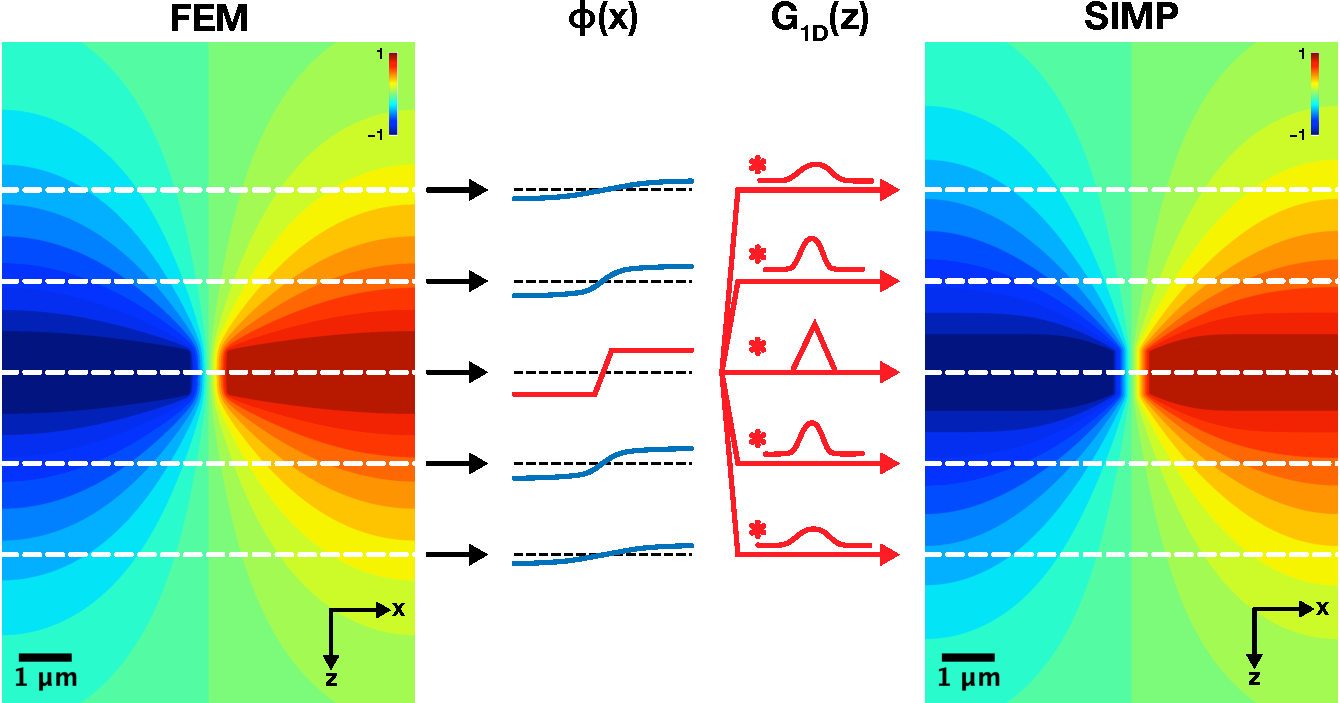
\includegraphics[width=\textwidth]{Figures/Schematics/SIMP-basic-idea.pdf}
	\caption{Schematic illustration of the mathematical foundation behind \emph{SIMP}. The line profiles $\phi\left(x\right)$ (indicated by the dashed white lines) of the 2D~electrostatic potential $\phi$ obtained from FEM simulations show the expected behavior at different projection distances $z$ from the specimen. Taking the initial electrostatic potential distribution $\phi_0\left(x\right)$ (red curve) and calculating the convolution with a projection distance dependent (normalized) 1D Gaussian kernel $G_{\mathit{1D}}\left(z\right)$ according to \cref{eq:SIMP-electrostatic-potential-convolution} yields a similar 2D~electrostatic potential.}
	\label{fig:SIMP-basic-idea}
\end{figure}
Furthermore, $\widetilde{G}\left(x, x', z'\right)$ has to obey the boundary conditions:
\begin{equation}
	\eval{\phi\left(x, z\right)}_{z \to \infty} = \text{const.} \quad ; \quad \eval{\phi\left(x, z\right)}_{z = 0} = \phi_0 \left(x\right),
\end{equation}
which therefore means that:
\begin{equation}
	\label{eq:green-function-boundary-conditions}
	\eval{\widetilde{G}\left(x, x', z'\right)}_{z \to \infty} = \text{const.} \quad ; \quad \eval{\widetilde{G}\left(x, x', z'\right)}_{z \to 0} = \delta \left(x - x'\right).
\end{equation}
The (normalized) Gaussian distribution can be described as a delta sequence \cite{Jackson1999} whose standard deviation obeys $\eval{\sigma_G}_{z \to 0} = 0$ and therefore the second condition of \cref{eq:green-function-boundary-conditions}. Additionally, the first condition of \cref{eq:green-function-boundary-conditions} is trivially fulfilled by the Gaussian distribution.

Given an initial electrostatic potential distribution $\phi_0 \left(x\right)$, the 2D~electrostatic potential can therefore be calculated (according to \cref{eq:2D-electrostatic-poisson-green}) through a convolution:
\begin{equation}
  \label{eq:SIMP-electrostatic-potential-convolution}
  \phi \left(x, z\right) = \phi_0\left(x\right) * G_{\mathit{1D}}\left(z\right),
\end{equation}
where $G_{\mathit{1D}}\left(z\right)$ is a 1D~Gaussian kernel. Here, the standard deviation $\sigma_G$ of the convolution kernel is dependent on the projection distance $z$ and scales with a power of $\ln\left(2\right)$ inside the stray field.

\emph{SIMP} consequently allows for the description of complex electrostatic problems, requiring minimal knowledge of the specimen besides an initial electrostatic potential distribution (which is given through simple analytical formulas for most geometric layouts and specimens) while significantly cutting down on computational complexity. Additionally, \emph{SIMP} offers the advantage that the computation of the 2D~electrostatic potential is done row by row, where each $\phi \left(x, z\right)$ does not depend on the previous result, allowing the computation to be parallelized and scale linearly with the available computational power.
\newpage
\section{Coplanar Capacitor} \label{sec:coplanar-capacitor-SIMP-EH-comparison}
In order to verify the validity of the presented model, the coplanar capacitor (\cref{fig:specimen-capacitor-layout}) described in \cref{ssec:2d-modeling-specimen}, whose physical behavior is well understood, is modeled and compared using both FEM simulations and \emph{SIMP}. These findings are used to compare the results obtained from \emph{SIMP} with experimental data obtained from off-axis EH and electron tomography.
\subsection{Comparison with Finite Element Method Simulations}
Due to the axial symmetry, only half of the problem's geometry, as described in \cref{ssec:2d-modeling-specimen}, needs to be modeled using FEM simulations and \emph{SIMP} (\cref{fig:capacitor-FEM-SIMP-comparison}), where appropriate adjustments were again made to account for the symmetry of the problem.
\begin{figure}[H]
	\centering
	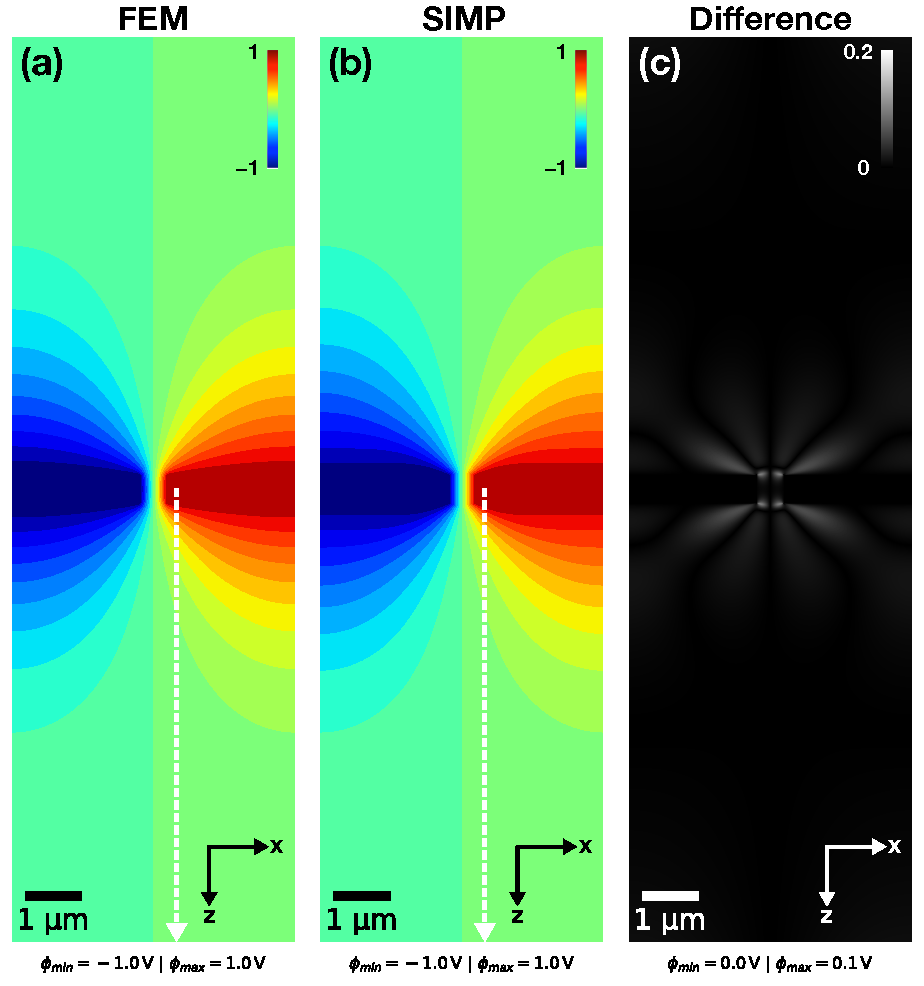
\includegraphics[width=0.8\textwidth]{Figures/Results/Capacitor/Simulations/capacitor-FEM-SIMP-comparison.pdf}
	\caption{Comparison between the 2D~electrostatic potential $\phi$ of the coplanar capacitor obtained from (a) the FEM simulation and (b) \emph{SIMP} along with (c) their absolute difference.}
	\label{fig:capacitor-FEM-SIMP-comparison}
\end{figure}
The electrostatic potential within the specimen region (i.\,e.\ for $\lvert z \rvert \le t = \SI{250}{\nm}$) is fully defined by the initial electrostatic potential distribution $\phi_0\left(x\right)$. Here, $\phi_0\left(x\right)$ is comprised of a constant potential $\phi_0\left(x\right) = \pm U_{\mathit{ext}}$ within the contacts and a linear slope between them. For $\lvert z \rvert \le t = \SI{250}{\nm}$ (i.\,e.\ for propagation distances starting at the specimen edge and extending into the vacuum region), $\phi \left(x, z\right)$ is calculated according to \cref{eq:SIMP-electrostatic-potential-convolution} from a convolution with a propagation distance dependent Gaussian kernel, where the kernel scales with a power of $\ln\left(2\right)$ and the standard deviation $\sigma_G$ ranges from $\sigma_G^{\mathit{min}} = \SI{1}{\nm}$ to $\sigma_G^{\mathit{max}} = \SI{4000}{\nm}$.

By comparing the 2D~electrostatic potential $\phi$ obtained from the FEM simulation (\cref{fig:capacitor-FEM-SIMP-comparison}a) with the one obtained from \emph{SIMP} (\cref{fig:capacitor-FEM-SIMP-comparison}b), it is apparent that presented model is in excellent agreement with well established simulation methods. As in the case with the FEM simulation, it is evident that the stray field extends well beyond the edge of the specimen into the vacuum region. Furthermore, by calculating the absolute difference of the two electrostatic potentials (\cref{fig:capacitor-FEM-SIMP-comparison}c), it is observed that the maximum deviation of $\Delta \phi_{\mathit{max}} = \SI{0.1}{\volt}$ is limited only to an area close to the contacts, where the approximations made in \cref{eq:poisson-equation-2D-approximation} are no longer valid for small $z$.
\newpage
Similar to \cref{ssec:experimental-results-capacitor-FEM-simulation}, the phase $\varphi$ can be obtained from the projection of the electrostatic potential (\cref{fig:capacitor-FEM-SIMP-linescan-comparison}a). Here it is evident that the phases (without any weighting applied to the different specimen regions), which were both offset to zero through subtraction by the first value, likewise exhibit minimal deviations. As already noted in \cref{ssec:experimental-results-capacitor-FEM-simulation}, the specimen (i.e. the region inside and between the contacts) only contributes a small part to the total phase (approximately 8\% of the maximum phase shift), which is predominantly made up of the stray field contribution. Additionally, the line profiles $\phi\left(z\right)$ of the electrostatic potential in propagation direction (indicated by the white dashed lines in \cref{fig:capacitor-FEM-SIMP-comparison}a and b) also demonstrate excellent agreement between the FEM simulation and \emph{SIMP}, with both line profiles approaching $\lim_{z\to\SI{8000}{\nm}} \phi\left(z\right) = \SI{0}{\volt}$.
\begin{figure}[H]
	\centering
	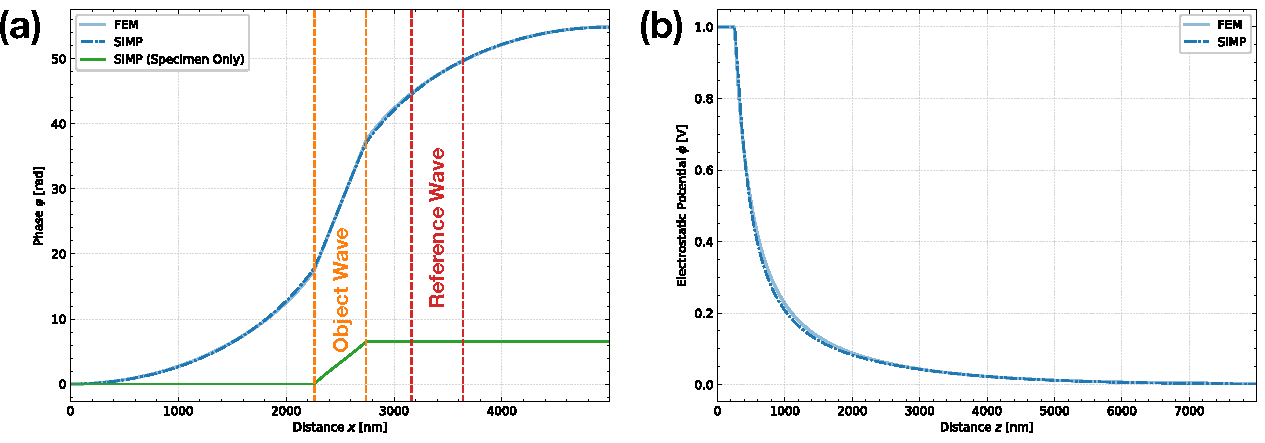
\includegraphics[width=\textwidth]{Figures/Results/Capacitor/Simulations/capacitor-FEM-SIMP-linescan-comparison.pdf}
	\caption{Comparison between the FEM simulation and \emph{SIMP} for the coplanar capacitor with (a) the phases $\varphi$ obtained through a projection of the 2D~electrostatic potential $\phi$ (with the object and reference wave indicated by the dashed orange and red lines) and (b) the line profiles $\phi\left(z\right)$ of the electrostatic potential in propagation direction (indicated by the white dashed lines in \cref{fig:capacitor-FEM-SIMP-comparison}a and b).}
	\label{fig:capacitor-FEM-SIMP-linescan-comparison}
\end{figure}
Considering the line profiles in \cref{fig:capacitor-FEM-SIMP-linescan-comparison}b, it is evident that the electrostatic potential calculated with \emph{SIMP} features the expected decay proportional to $1/z$. Furthermore, the plateau region at the beginning of both line profiles reflects the constant potential for $\lvert z \rvert \le t = \SI{250}{\nm}$ given from the initial potential distribution $\phi_0 \left(x\right)$, where the origin $z_0 = \SI{0}{\nm}$ for both line profiles lies precisely in the middle of the contacts.

Examining the line profiles further confirms the aforementioned findings, where the stray field extends well beyond the specimen edge into the vacuum region and accounts for much of the overall phase, with the electrostatic potential dropping to 10\% of its initial value of $U_{\mathit{ext}} = \pm \SI{1.0}{\volt}$ after a propagation distance of $z \approx \SI{2000}{\nm}$.

While the agreement between the FEM simulation and \emph{SIMP} for an identical specimen geometry seems promising at first, the question of the robustness of the presented model still arises. In order to verify this, it is investigated whether the same excellent agreement is achieved for a modified specimen geometry, all other parameters being equal.
\newpage
For this purpose, the distance between the capacitor plates $d$, with otherwise unchanged specimen geometry and simulation parameters, is modified to $d = \SI{960}{\nm}$ and $d = \SI{240}{\nm}$ (i.\,e.\ exactly double and half the above described distance $d$), respectively, and the deviation between the two models is investigated (\cref{fig:capacitor-FEM-SIMP-comparison-varying-distance}). To be precise, it is of interest whether a modified specimen geometry continues to produce the small deviations observed above between the two models while keeping the parameters with respect to the standard deviation of the Gaussian kernel $\sigma_G$ and the initial electrostatic potential distribution $\phi_0\left(x\right)$ unchanged.
\begin{figure}[H]
	\centering
	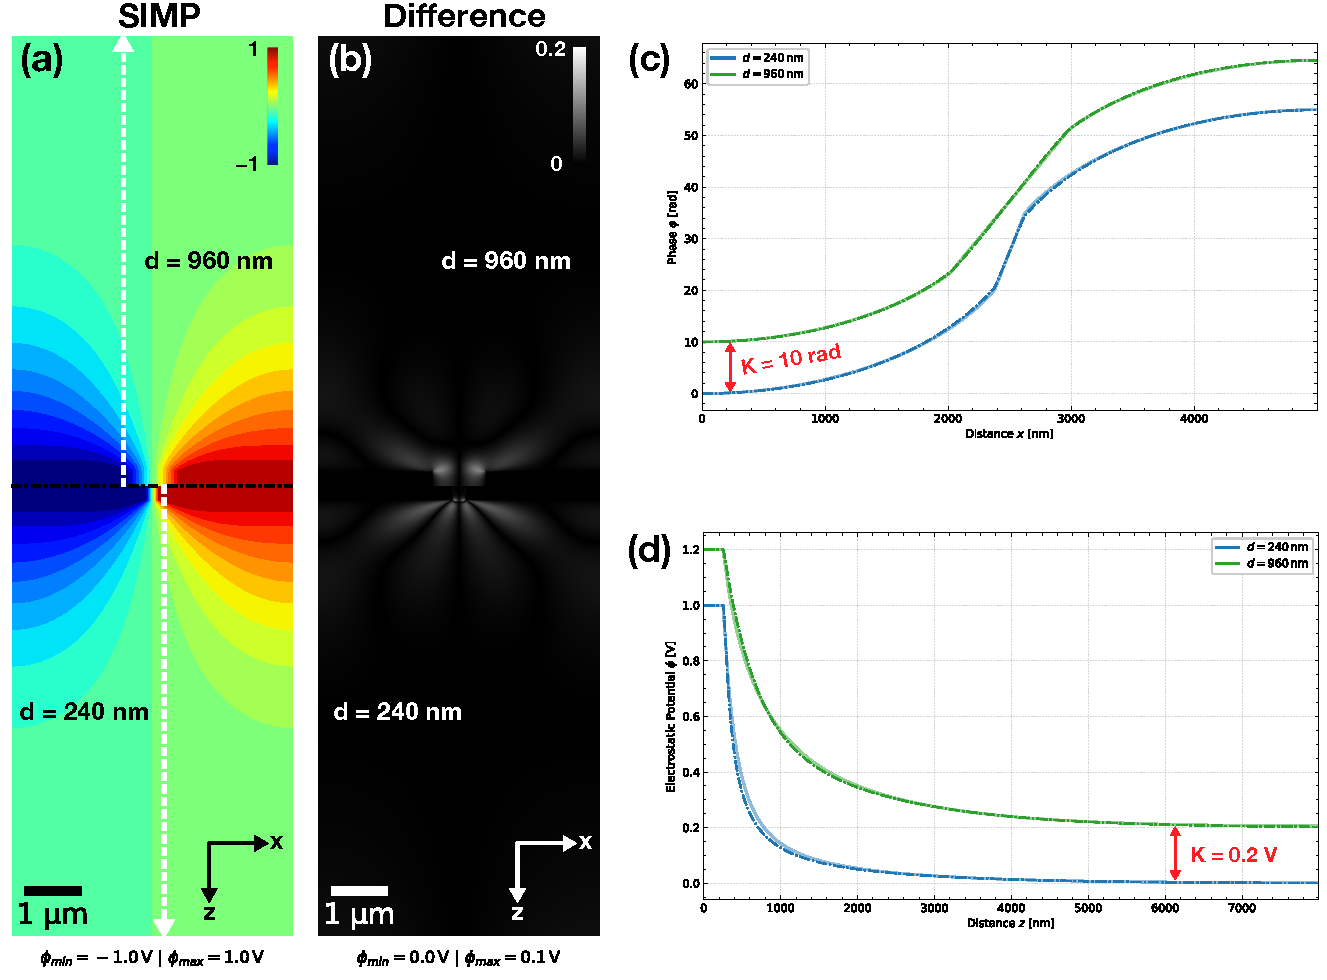
\includegraphics[width=\textwidth]{Figures/Results/Capacitor/Simulations/capacitor-FEM-SIMP-comparison-varying-distance.pdf}
	\caption{Comparison between the FEM simulation and \emph{SIMP} for the coplanar capacitor with (a) the 2D~electrostatic potential obtained from \emph{SIMP} for a distance between the capacitor plates of $d = \SI{960}{\nm}$ (upper half) and $d = \SI{240}{\nm}$ (lower half), their absolute differences in upper and lower half of (b), respectively, (c) the phases $\varphi$ obtained through a projection of the 2D~electrostatic potential $\phi$ and (d) the line profiles $\phi\left(z\right)$ of the electrostatic potential in propagation direction (indicated by the white dashed lines in a).}
	\label{fig:capacitor-FEM-SIMP-comparison-varying-distance}
\end{figure}
For the 2D~electrostatic potentials calculated from \emph{SIMP}, a behavior resembling the one mentioned above can also be observed for $d = \SI{960}{\nm}$ and $d = \SI{240}{\nm}$ (\cref{fig:capacitor-FEM-SIMP-comparison-varying-distance}a). Specifically, a modified specimen geometry with respect to the distance of the capacitor plates appears to result in negligible variations in the electrostatic potential beyond the immediate vicinity of the capacitor plate corners. For both plate distances, it can further be noted that the stray field extends far beyond the specimen edge into the vacuum. These minor variations in electrostatic potential due to modification of the specimen geometry are likewise reflected in the absolute difference between the FEM simulation and \emph{SIMP} (\cref{fig:capacitor-FEM-SIMP-comparison-varying-distance}b), where for both plate distances the maximum deviation does not exceed the previously observed value of $\Delta \phi_{\mathit{max}} = \SI{0.1}{\volt}$ and is likewise only located close to the contacts.

As with the original specimen geometry, the phase $\varphi$ can be calculated for both plate distances from a projection of the electrostatic potential (\cref{fig:capacitor-FEM-SIMP-comparison-varying-distance}c). For both plate distances $d = \SI{960}{\nm}$ and $d = \SI{240}{\nm}$ it is apparent that the FEM simulation and \emph{SIMP} are still in excellent agreement. The same observation is supported by the line profiles $\phi\left(z\right)$ of the electrostatic potential in propagation direction (\cref{fig:capacitor-FEM-SIMP-comparison-varying-distance}d, indicated by the white dashed lines in \cref{fig:capacitor-FEM-SIMP-comparison-varying-distance}a), where both line profiles likewise approach $\lim_{z\to\SI{8000}{\nm}} \phi\left(z\right) = \SI{0}{\volt}$.

In order to improve the visibility of the plotted phases, the phase for $d = \SI{240}{\nm}$ was offset to zero through subtraction by the first value, while the phase for $d = \SI{960}{\nm}$ was offset to $K = \SI{10}{rad}$. The same adjustments was made for the line profiles of the electrostatic potential, where the line profile for $d = \SI{960}{\nm}$ was offset by $K = \SI{0.2}{\volt}$ relative to line profile for $d = \SI{240}{\nm}$.

These preliminary findings (utilizing the coplanar capacitor as a reference specimen) suggest that \emph{SIMP} is a simple, yet promising, approach for the approximate modeling of electrostatic potential distributions. In order to verify the validity of the model, however, further comparisons with real-world measurements are needed, as detailed in the following \cref{ssec:experimental-results-SIMP-EH-comparison,ssec:capacitor-SIMP-tomography-comparison}.
\newpage
\subsection{Comparison with Off-Axis Electron Holography} \label{ssec:experimental-results-SIMP-EH-comparison}
Similar to \cref{ssec:experimental-results-capacitor-FEM-simulation}, comparisons are made with the experimentally obtained data described in \cref{ssec:experimental-results-capacitor-EH} (\cref{fig:capacitor-SIMP-EH-linescan-comparison}). Here, the object wave $\varphi_{\mathit{obj}}$ corresponds to the vacuum region between the contacts (\cref{fig:capacitor-FEM-SIMP-linescan-comparison}a, indicated by the dashed orange lines) and the reference wave $\varphi_{\mathit{ref}}$ to a region of the same size offset $\SI{800}{\nm}$ to the right (\cref{fig:capacitor-FEM-SIMP-linescan-comparison}a, indicated by the dashed red lines).
\begin{figure}[H]
	\centering
	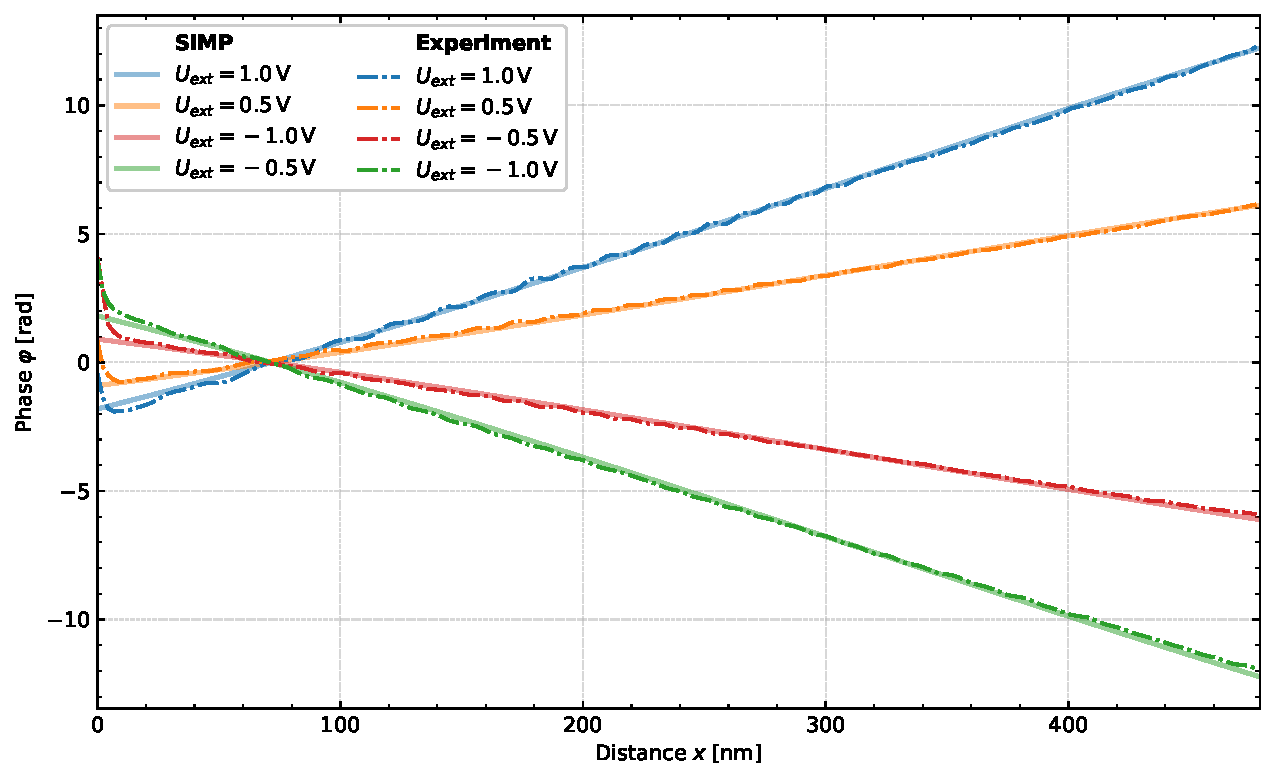
\includegraphics[width=\textwidth]{Figures/Results/Capacitor/Simulations/capacitor-SIMP-EH-linescan-comparison.pdf}
	\caption{Comparison between the phases $\varphi$ obtained from the experimentally acquired holograms (dashdotted lines) and those calculated with \emph{SIMP} (solid lines) for different bias voltages, where the reference wave $\varphi_{\mathit{ref}}$ is subtracted from the object wave $\varphi_{\mathit{obj}}$ according to the regions illustrated in \cref{fig:capacitor-FEM-SIMP-linescan-comparison}.}
	\label{fig:capacitor-SIMP-EH-linescan-comparison}
\end{figure}
As is the case with the FEM simulation, the simulated phases $\varphi$ obtained from \emph{SIMP} are in excellent agreement with the experimental phases acquired through off-axis EH for all external bias voltages $U_{\mathit{ext}}$, ranging from $\SIrange{-1.0}{1.0}{\volt}$ in increments of $\SI{0.5}{\volt}$, further supporting the validity of the proposed model.\footnote{Since the simulated coplanar capacitor was electrically biased by applying $\pm U_{\mathit{ext}}$ at the contacts, while the experimentally measured capacitor was grounded at one of the contacts, a scaling factor of $2$ has been applied when calculating the phase through projection.}

As before, the experimentally acquired 2D~phase images were modulated by subtracting a phase wedge (\cref{eq:holosuite-phase-wedge,eq:holosuite-phase-wedge-average-fit}).
\newpage
\subsection{Comparison with Electron Tomography} \label{ssec:capacitor-SIMP-tomography-comparison}
Due to its ability to obtain detailed structures of the investigated specimen in propagation direction, (electron) tomographic reconstruction represents a powerful measurement technique (a detailed description of the mathematical foundation behind (electron) tomography is given in \cref{sec:electron-tomography}). To be precise, the ability to obtain $n$-dimensional phase maps from $k$ $\left(n - 1\right)$ dimensional phase images (\cref{fig:TEM-tomography-capacitor-setup}) opens the door for the investigation of 3D~electric and magnetic properties of specimens on the nanometer scale and below.
\begin{figure}[H]
	\centering
	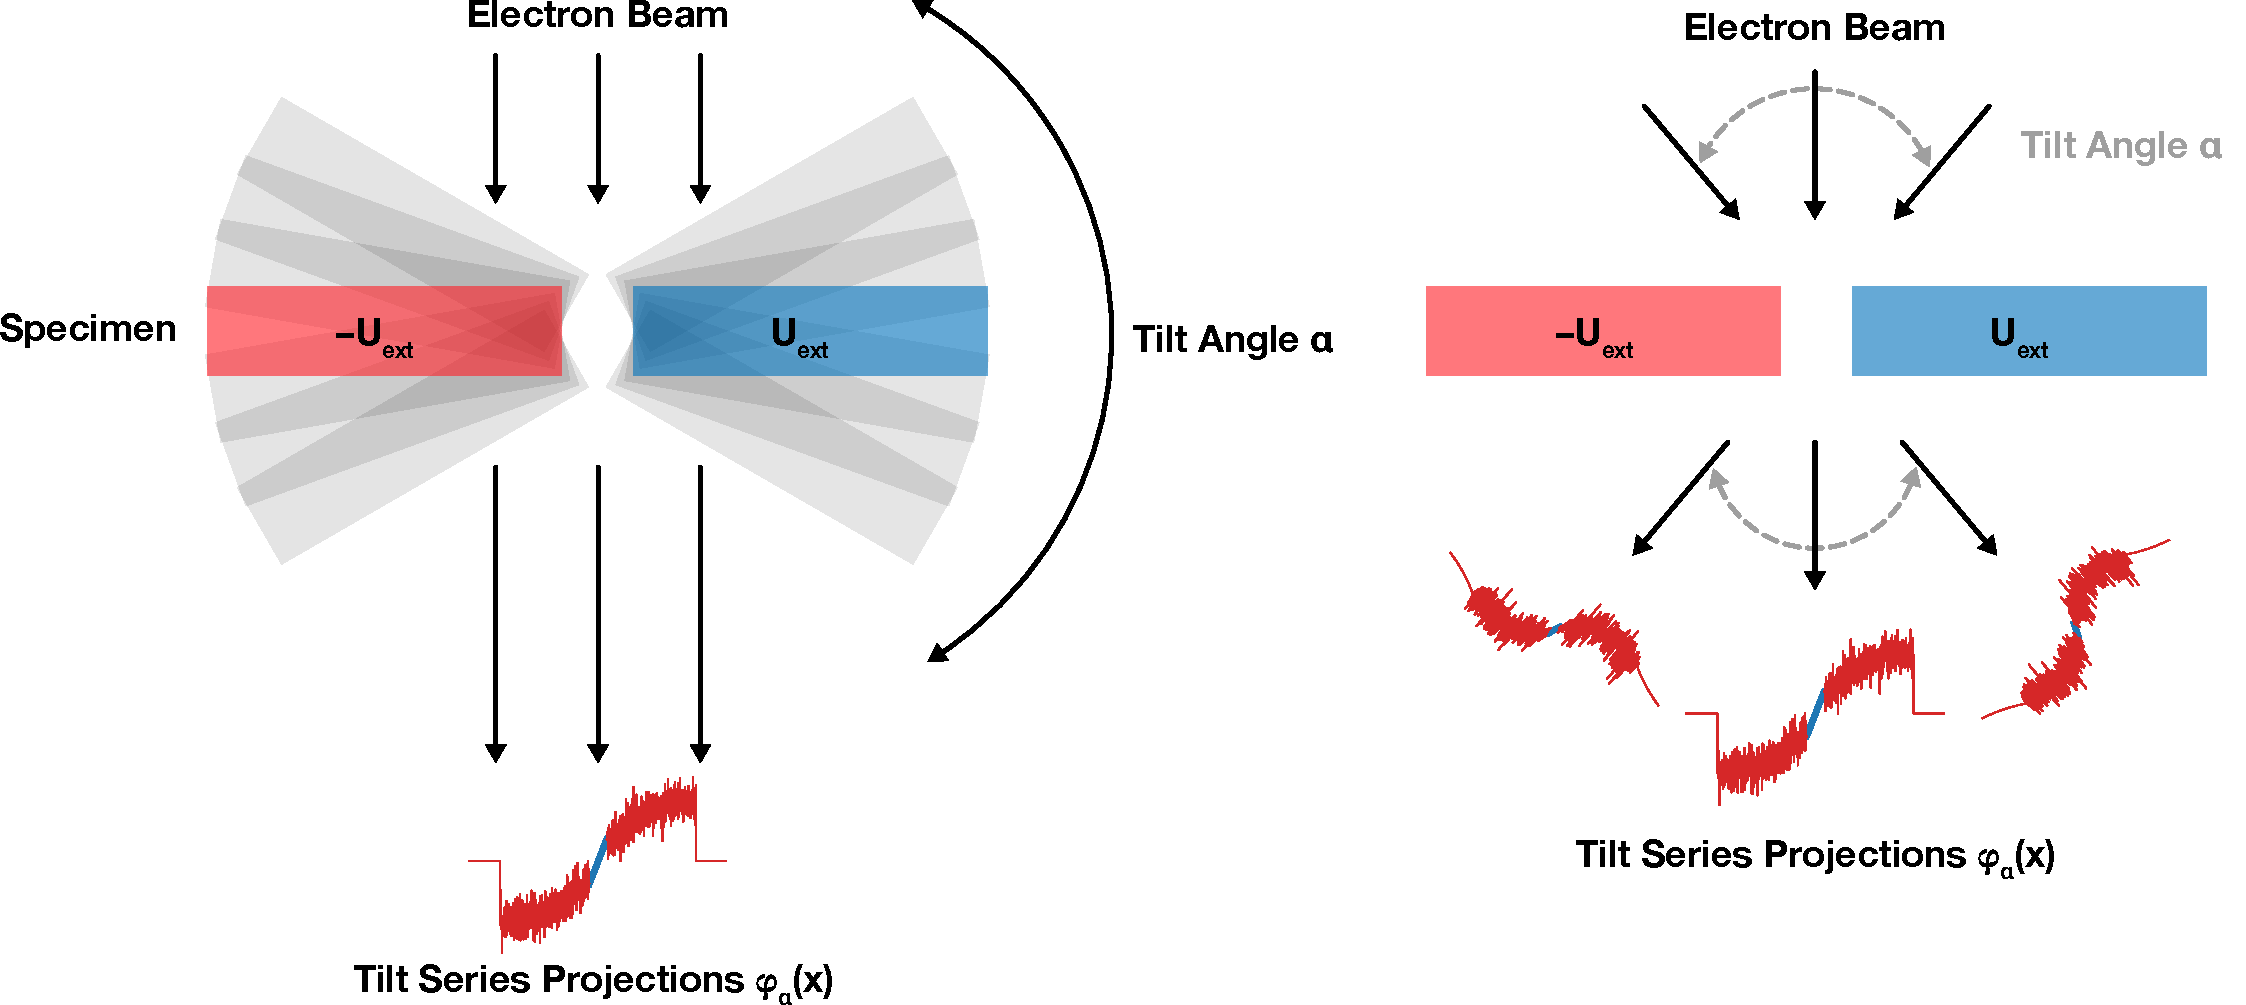
\includegraphics[width=\textwidth]{Figures/Schematics/Theoretical Foundations/TEM-tomography-capacitor-setup.pdf}
	\caption{Schematic illustration of the tomographic measurement process of the coplanar capacitor. The electron beam propagates through the specimen, which is rotated by a tilt angle $\alpha$, and generates the tilt series projection $\varphi_{\alpha}\left(x\right)$ on the detector. Since the capacitor plates are non-transparent, they cast a shadow on the detector when projected, necessitating that these areas of the projection be zeroed (illustrated by the red lines in the tilt series projections) so that the information between the electrodes (illustrated by the blue lines in the tilt series projections) remains.}
	\label{fig:TEM-tomography-capacitor-setup}
\end{figure}
In electron holographic tomography, by tilting the coplanar capacitor, a 2D~electron hologram is recorded for each tilt angle $\alpha$ (\cref{fig:TEM-tomography-capacitor-setup}), which is subsequently reconstructed as described in \cref{ssec:holosuite-automated-reconstruction}. For the phase images $\varphi$ obtained from this, a line profile between the capacitor plates is calculated for each of them as described in \cref{ssec:experimental-results-capacitor-EH}, where the composition of these 1D~line profiles $\varphi_{\alpha}\left(x\right)$ yields the 2D~sinogram $\hat{f}\left(\alpha, \varphi\right)$. In the case of the simulated 2D~electrostatic potential distributions, the 1D~line profiles follow directly from the projection through the Radon transform. The line profiles are subsequently offset to zero by subtracting their center value. Furthermore, all line profiles are zeroed in the area corresponding to the capacitor plates, reflecting the shadow the contacts cast due to their thickness (\cref{fig:TEM-tomography-capacitor-setup}, illustrated by the red lines in the tilt series projections). To do so, a linear fit between the capacitor plates is calculated and extrapolated to the whole projection, from which the capacitor plate edges can be detected with a threshold value for the deviation from the line profiles.
\newpage
In order to compare the above detailed results obtained from \emph{SIMP} with tomographically reconstructed phase images, the validity of the underlying Radon transform (\cref{eq:2D-radon-transform}) applied to the coplanar capacitor has to be verified first. For this purpose, the 2D~electrostatic potential obtained from \emph{SIMP} is Radon transformed by means of projection in an angular range of $\alpha = \pm \SI{90}{\degree}$ in $\SI{1}{\degree}$ increments, where the resulting sinogram is inverse radon transformed (\cref{fig:capacitor-SIMP-tomography-comparison}).
\begin{figure}[H]
	\centering
	\includegraphics[width=\textwidth]{Figures/Results/Capacitor/Tomography/capacitor-SIMP-tomography-comparison.pdf}
	\caption{Tomographic reconstruction utilizing \emph{scikit-image}'s implementation \cite{Vanderwalt2014} of the Radon transform (\cref{eq:2D-radon-transform}) with (a) the 2D~electrostatic potential $\phi$ obtained from \emph{SIMP}, (b) the sinogram $\hat{f}\left(\alpha, \varphi\right)$ calculated through projection (with the input assumed to be zero outside the inscribed circle), (c) the resulting tomographically reconstructed 2D~electrostatic potential $\phi_{\mathit{rec}}$ and (d) the same tomographic reconstruction $\phi_{\mathit{rec}}^{\mathit{rest}}$ with real-world like limitations and a 2D~Gaussian blur of $\sigma_G = 4.0$ applied.}
	\label{fig:capacitor-SIMP-tomography-comparison}
\end{figure}
It is observed that the sinogram $\hat{f}\left(\alpha, \varphi\right)$ (\cref{fig:capacitor-SIMP-tomography-comparison}b) following from the 2D~electrostatic potential (\cref{fig:capacitor-SIMP-tomography-comparison}a) results in a 2D~electrostatic potential which is in excellent agreement with the initially provided potential distribution (\cref{fig:capacitor-SIMP-tomography-comparison}c). The low noise observed in some areas of the tomographic reconstruction is the result of reconstruction artifacts in the Fourier transform of the filtered back projection (FBP), where a ramp filter was used in this case.

These observations validate tomographic reconstruction as a suitable measurement and analysis technique for the specimens described here. Furthermore, they demonstrate that the FBP is sufficiently accurate to yield results that match the input potential distribution of these specimens (\cref{fig:capacitor-SIMP-tomography-linescan-comparison}), thereby alleviating the need for computationally expensive iterative reconstruction schemes.

However, since real-world measurements possess several limitations, it is of interest to see how these constraints affect the tomographic reconstruction of the same 2D~electrostatic potential. In detail, it is of interest how a restriction of the tilt series to an angular range of $\alpha = \pm \SI{34}{\degree}$ in $\SI{2}{\degree}$ increments as well as a zeroing of the projection in the region of the capacitor plates affects the tomographic reconstruction. To better approximate the behavior observed in the experimental measurements, the 2D~electrostatic potential inside the contacts of the coplanar capacitor is replaced with random noise, where the values are an order of magnitude larger than externally applied bias.
\begin{figure}[H]
	\centering
	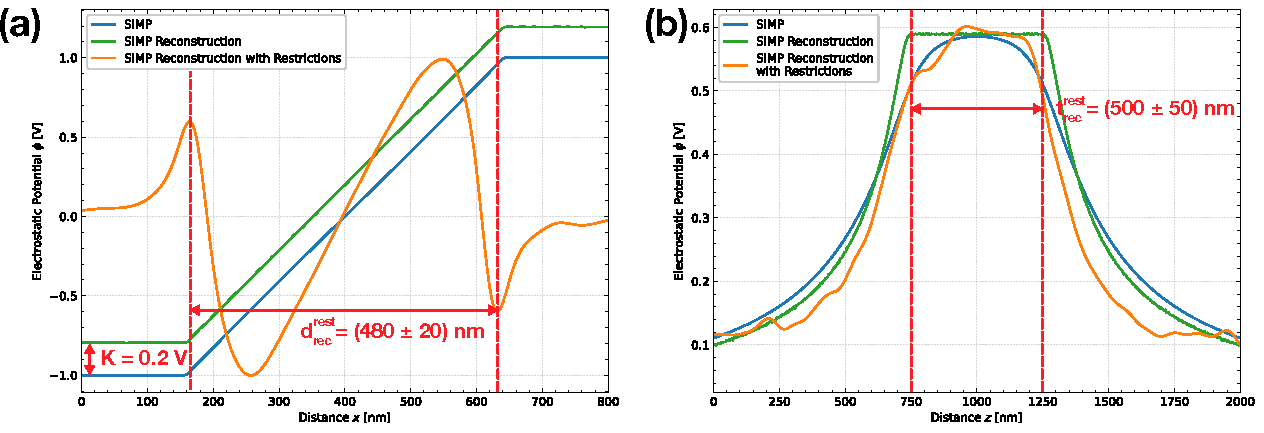
\includegraphics[width=\textwidth]{Figures/Results/Capacitor/Tomography/capacitor-SIMP-tomography-linescan-comparison.pdf}
	\caption{Comparison between the input 2D~electrostatic potential $\phi$ of the coplanar capacitor obtained from \emph{SIMP} and the tomographically reconstructed potential distributions $\phi_{\mathit{rec}}$ and $\phi_{\mathit{rec}}^{\mathit{rest}}$ with (a) the line profiles $\phi\left(x\right)$ across center of the specimen and (b) the line profiles $\phi\left(z\right)$ across the right contact (with both line profiles indicated by the solid and dashed white lines in \cref{fig:capacitor-SIMP-tomography-comparison}, respectively).}
	\label{fig:capacitor-SIMP-tomography-linescan-comparison}
\end{figure}
Here, it is apparent that the limited angular range of the tilt series (i.\,e.\ missing wedge) and the zeroing of the projection in the region of the capacitor plates (i.\,e.\ interior Radon transform) have a considerable impact on the tomographic reconstruction, which is especially noticeable in the limited spatial resolution in $z$-direction and almost completely missing information outside the region between the contacts (\cref{fig:capacitor-SIMP-tomography-comparison}d). Despite these severe limitations, the spacing of the capacitor plates can still be determined to be $d_{\mathit{rec}}^{\mathit{rest}} = \SI{480 \pm 20}{\nm}$ (\cref{fig:capacitor-SIMP-tomography-linescan-comparison}a, indicated by the red line) and the thickness of the specimen to be $t_{\mathit{rec}}^{\mathit{rest}} = \SI{500 \pm 50}{\nm}$ (\cref{fig:capacitor-SIMP-tomography-linescan-comparison}b, indicated by the red line), within whose measurement uncertainties the actual simulated values of $d = \SI{480}{\nm}$ and $t = \SI{500}{\nm}$ lie.

The deviation in slope as well as the ringing artifacts observed in the line profile of the restricted tomographic reconstruction $\phi_{\mathit{rec}}^{\mathit{rest}}\left(x\right)$ (\cref{fig:capacitor-SIMP-tomography-linescan-comparison}a) are likewise due to reconstruction artifacts arising from the previously mentioned real-world limitations (i.\,e.\ missing wedge, interior Radon transform and zeroing of the projection due to the shadow cast by the contacts).
\newpage
In order to improve the visibility of the plotted line profiles, the electrostatic potential $\phi_{\mathit{rec}}\left(x\right)$ obtained from the tomographic reconstruction of \emph{SIMP} without restrictions is offset by $K = \SI{0.2}{\volt}$.

These findings further suggest that the chosen angular resolution of $\Delta \alpha = \SI{2}{\degree}$ is sufficient enough to resolve the desired specimen features \cite{Yalisove2021}, where the achievable spacial resolution is given by the Crowther criterion \cite{Bracewell1967,Crowther1970}.

Having demonstrated the general validity of the tomographic reconstruction technique using the coplanar capacitor modeled with \emph{SIMP}, these results are compared to the tomographic reconstruction of the experimentally recorded holograms (\cref{fig:capacitor-SIMP-EH-tomography-comparison}).
\begin{figure}[H]
	\centering
	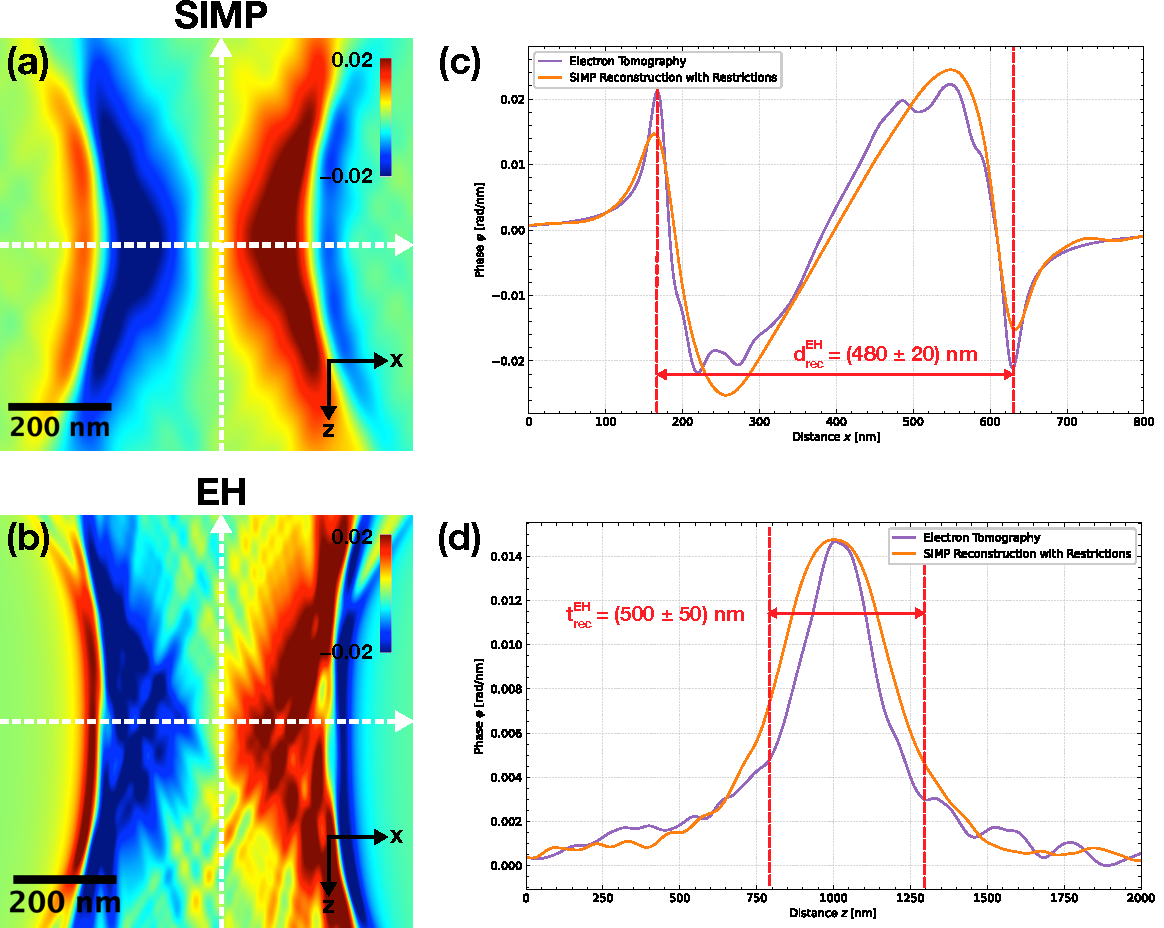
\includegraphics[width=\textwidth]{Figures/Results/Capacitor/Tomography/capacitor-SIMP-EH-tomography-comparison.pdf}
	\caption{Tomographic reconstruction of the coplanar capacitor with (a) the 2D~back-projected phase $\varphi_{\mathit{rec}}^{\mathit{rest}}$ obtained from \emph{SIMP}, (b) the 2D~back-projected phase $\varphi_{\mathit{rec}}^{\mathit{EH}}$ obtained from the experimentally acquired holograms, (c) the line profiles $\varphi\left(x\right)$ across the center of the specimen and (d) the line profiles $\varphi\left(z\right)$ across the right contact. For both 2D~back-projected phases, a 2D~Gaussian Blur of $\sigma_G = 4.0$ is applied.}
	\label{fig:capacitor-SIMP-EH-tomography-comparison}
\end{figure}
Considering the line profiles $\varphi\left(x\right)$, it is observed that, although the experimentally recorded data exhibits a noticeable degree of noise, the spacing of the capacitor plates can still be determined to be $d_{\mathit{rec}}^{\mathit{EH}} = \SI{480 \pm 20}{\nm}$ (\cref{fig:capacitor-SIMP-EH-tomography-comparison}c, indicated by the red line), which, accounting for the measurement uncertainty, is in agreement with the value obtained from \emph{SIMP}. The same applies to the line profiles $\varphi\left(z\right)$, where, despite the visible noise of the experimental data, the specimen thickness is determined to be $t_{\mathit{rec}}^{\mathit{EH}} = \SI{500 \pm 50}{\nm}$ (\cref{fig:capacitor-SIMP-EH-tomography-comparison}d, indicated by the red line), which, in the context of the measurement uncertainty, is in agreement with the value obtained from \emph{SIMP}. In general, both the 2D~back-projected phases (\cref{fig:capacitor-SIMP-EH-tomography-comparison}a and b) and the line profiles (\cref{fig:capacitor-SIMP-EH-tomography-comparison}c and d, indicated by the dashed white lines in \cref{fig:capacitor-SIMP-EH-tomography-comparison}a and b) showcase excellent agreement between the experimentally acquired holograms and the simulated specimen, further validating \emph{SIMP} as a suitable modeling approach for the approximation of electrostatic potential distributions.
\newpage
\section{Extension to Semiconductor Nanostructures}
After validating the underlying approach of the presented model in the previous \cref{sec:coplanar-capacitor-SIMP-EH-comparison} using the coplanar capacitor as a reference specimen, this chapter extends the presented model to semiconductor nanostructures using a multi-layer framework. This extension enables the study of the electrostatic potential distribution within doped semiconductor nanostructures and its impact on off-axis EH, providing valuable information for the characterization and optimization of such nanoscale electronic devices.
\subsection[\texorpdfstring{$p$-$n$}{\textit{p}-\textit{n}}-Junction]{$\boldsymbol{p}$-$\boldsymbol{n}$-Junction} \label{ssec:SIMP-pn-junction-extension}
One of the simplest semiconductor nanostructures is the symmetrically doped $p$-$n$-junction, which is used for didactical reasons. However, it should be noted that for comparison with experimental data, the previously introduced $p$-$p^+$-$n^+$-junction is used. For this, similar to the geometric layout described in \cref{ssec:2d-modeling-specimen}, two Si~specimen regions are defined and modeled, where both the $p$-region and the $n$-region are doped with $\SI[per-mode=power]{1e19}{\per\cubic\cm}$ and have a width of $\SI{2500}{\nm}$ and thickness of $\SI{150}{\nm}$ each. Outside the specimen, a vacuum region of $\SI{2500}{\nm}$ is assumed, with the overall geometry of the model being $\SI{5000}{\nm} \times \SI{2650}{\nm}$. The axial symmetry of the problem can again be exploited to reduce the computational complexity of the problem by modeling only half of the specimen's geometry.

Contrary to the coplanar capacitor, the initial electrostatic potential distribution $\phi_0\left(x\right)$ is not given by a constant potential at both contacts and a linear gradient in between, but rather by \cref{eq:pn-junction-potential}. With this initial electrostatic potential distribution, the 2D~electrostatic potential $\phi$, similar to the coplanar capacitor, can be calculated using \cref{eq:SIMP-electrostatic-potential-convolution}, where the standard deviation $\sigma_G$ of the projection distant dependent (normalized) 1D~Gaussian convolution kernel scales with a power of $\ln\left(2\right)$ outside the specimen (\cref{fig:pn-junction-SIMP-multilayer-EH-comparison}).

Comparing the 2D~electrostatic potential $\phi_{\mathit{SL}}$ obtained from \emph{SIMP} within the single-layer framework (\cref{fig:pn-junction-SIMP-multilayer-EH-comparison}a) with the experimentally acquired holograms of the $p^+$-$n^+$-junction through their phases $\varphi$ (i.\,e.\ a projection in propagation direction), it is apparent that the single-layer model fails to accurately describe the experimentally acquired holograms (\cref{fig:pn-junction-SIMP-multilayer-EH-comparison}d). Not only is the observable phase jump of the single-layer model more than twice as large as the experimentally acquired one, but the width of the depletion region $\omega$ (which follows from \cref{eq:depletion-region-width-n-region,eq:depletion-region-width-p-region}) obtained from \emph{SIMP} is also an order of magnitude smaller than the experimentally observed one.
\newpage
The primitive single-layer model, as is the case with the \emph{nextnano} simulations, assumes a specimen that has suffered no sub-surface preparation damage and is therefore not able to accurately describe the kinds of specimens investigated in a TEM. These observations consequently necessitate the need for a multi-layer framework that takes these various preparation damage effects into account while still requiring minimal knowledge about the microscopic charge carrier distribution.
\begin{figure}[H]
	\centering
	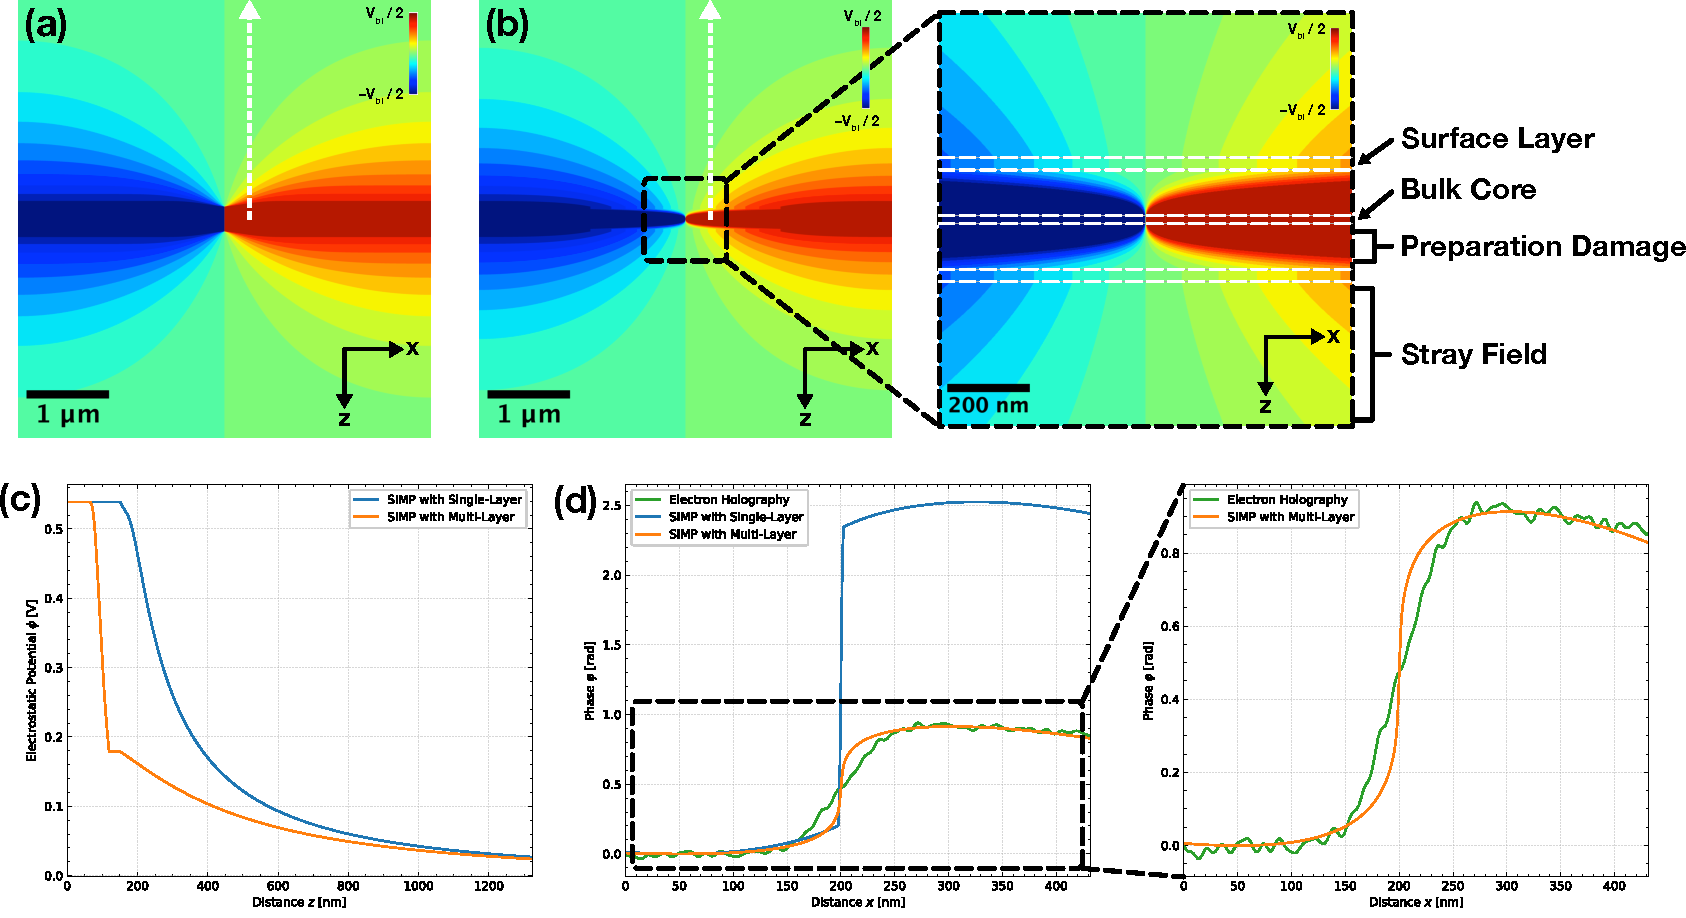
\includegraphics[width=\textwidth]{Figures/Results/pn-Junction/Simulations/pn-junction-SIMP-multilayer-EH-comparison.pdf}
	\caption{Comparison between the differently layered \emph{SIMP} frameworks for the symmetrically doped $p$-$n$-junction with (a) the 2D~electrostatic potential $\phi_{\mathit{SL}}$ obtained from the single-layer model, (b) the 2D~electrostatic potential $\phi_{\mathit{ML}}$ obtained from the multi-layer model, (c) the corresponding line profiles $\phi\left(z\right)$ in propagation direction (indicated by the white dashed lines in a and b) and (d) the phases $\varphi$ obtained through a projection of $\phi$ compared with the experimentally acquired holograms.}
	\label{fig:pn-junction-SIMP-multilayer-EH-comparison}
\end{figure}
As indicated in \cref{ssec:experimental-results-pnjunction-FEM-simulation}, the FIB preparation stage generates Ga-induced defects resulting in an electrically damaged crystalline layer below the electrically inactive surface layer \cite{Twitchett2002,Beleggia2003,Cooper2006,Cooper2007,Twitchett-Harrison2007,Cooper2009,Somodi2013,Yazdi2015}. As such, the specimen can be divided into three different regions:
\begin{itemize}
	\item \textbf{Bulk Core:} The 2D~electrostatic potential $\phi_{\mathit{ML}}$ follows the classical bulk theory for a $p$-$n$-junction (given by \cref{eq:pn-junction-potential}) and is given by the initial electrostatic potential distribution $\pdv*{\phi_0\left(x\right)}{z} = \text{const.}$;
	\item \textbf{Preparation Damage:} Here, the specimen suffers preparation damage due to the ion implantation by the FIB over an implantation depth $t_{\mathit{PD}}$. The degree of damage depends, among other things, on parameters such as the accelerating voltage $U_{\mathit{acc}}$ of the FIB and the atomic number $Z$ of the ions used for milling. The 2D~electrostatic potential $\phi_{\mathit{ML}}$ follows, similar to \cref{eq:SIMP-electrostatic-potential-convolution}, through a convolution of the bulk core potential distribution $\phi_0\left(x\right)$ with a projection distant dependent 1D~Gaussian kernel $G_{\mathit{1D}}\left(z\right)$;
	\item \textbf{Surface Layer:} This region represents an electrically inactive amorphous transition layer between the preparation damage region and the stray field. Here, the 2D~electrostatic potential $\phi_{\mathit{ML}}$ is given by the outer edge of the preparation damage layer $\pdv*{\phi_{t_{\mathit{PD}}}\left(x\right)}{z} = \text{const.}$
\end{itemize}
Given this multi-layer framework for \emph{SIMP}, a total of three distances have to be defined: The bulk core thickness $t_{\mathit{BC}}$, the implantation depth of the preparation damage region~$t_{\mathit{PD}}$ and the amorphous surface layer thickness $t_{\mathit{SL}}$.

The thickness of the amorphous surface layer $t_{\mathit{SL}}$ can be experimentally determined by comparing convergent-beam electron diffraction (CBED) measurements with off-axis EH measurements (\cref{fig:CBED-comparison-simulation-thickness}, a detailed description of CBED can be found in \cref{chap:appendix-CBED}). In detail, the crystalline part of the specimen thickness is determined to be $t_{\mathit{CBED}} = \SI{270 \pm 2}{\nm}$, where the difference to the thickness of $t_{\mathit{EH}} = \SI{325 \pm 5}{\nm}$ measured with off-axis EH (\cref{chap:appendix-specimen-thickness-off-axis-EH}) yields the surface layer thickness of $t_{\mathit{SL}} = \SI{30 \pm 5}{\nm}$.

Using a surface layer thickness of $t_{\mathit{SL}} = \SI{30}{\nm}$ and a bulk core thickness of $t_{\mathit{BC}} = \SI{10}{\nm}$, the preparation damage region has a thickness of $t_{\mathit{PD}} = \SI{110}{\nm}$. With this, along with the same parameters for the stray field as before, the 2D~electrostatic potential~$\phi_{\mathit{ML}}$ can be calculated (\cref{fig:pn-junction-SIMP-multilayer-EH-comparison}b). The single-layer model and multi-layer model can then be compared through their corresponding line profiles $\phi\left(z\right)$ in propagation direction (indicated by the white dashed lines in \cref{fig:pn-junction-SIMP-multilayer-EH-comparison}a and b), where it is apparent that, while both models match inside the bulk core region (i.\,e.\ for $\lvert z \rvert \leq t_{\mathit{BC}}$) and approach $\lim_{z\to\SI{2650}{\nm}} \phi\left(z\right) = \SI{0}{\volt}$, the preparation damage region introduced in the multi-layer model causes the electrostatic potential distribution to decay considerable earlier compared to the single-layer model (\cref{fig:pn-junction-SIMP-multilayer-EH-comparison}c). Furthermore, by comparing the phase $\varphi$ of the multi-layer model (obtained through a projection of the electrostatic potential in propagation direction) to the experimentally acquired holograms, it is apparent that the multi-layer framework is in significantly greater agreement with the real-world measurements (\cref{fig:pn-junction-SIMP-multilayer-EH-comparison}d).

As described in \cref{ssec:FEM-simulated-potential-and-phase} the phases $\varphi$ obtained from \emph{SIMP} are calculated by subtracting the reference phase $\varphi_{\mathit{ref}}$, which only contains the stray field contribution, from the object phase $\varphi_{\mathit{obj}}$ (where both are separated by the biprism shadow) and modulating them through the subtraction of a phase wedge.
\newpage
\subsection[\texorpdfstring{$p$-$p^+$-$n^+$}{\textit{p}-\textit{p}\textsuperscript{+}-\textit{n}\textsuperscript{+}}-Junction]{$\boldsymbol{p}$-$\boldsymbol{p^+}$-$\boldsymbol{n^+}$-Junction} \label{ssec:SIMP-ppn-junction-extension}
Having established the validity of the multi-layer framework for \emph{SIMP} using a symmetrically doped $p$-$n$-junction in the previous \cref{ssec:SIMP-pn-junction-extension}, the same multi-layer model can now be extended to a $p$-$p^+$-$n^+$-junction.

For this, a Si~specimen with an geometric layout identical to \cref{fig:specimen-nextnano-layout} is modeled, where each doped region has a width of $\SI{1000}{\nm}$ and a thickness of $\SI{150}{\nm}$. The vacuum region outside the specimen extends for $\SI{2500}{\nm}$, for a total geometry of $\SI{3000}{\nm} \times \SI{2650}{\nm}$. As with the previous simulations, the axial symmetry of the problem is exploited to reduce the computational complexity of the simulation.

Identical to the above described specimen, the initial electrostatic potential distribution~$\phi_0 \left(x\right)$ at the junction between the $p^+$-region and $n^+$-region, which are both doped with $\SI[per-mode=power]{1e19}{\per\cubic\cm}$, is given by \cref{eq:pn-junction-potential}. The weakly doped (i.\,e.\ $\SI[per-mode=power]{1e16}{\per\cubic\cm}$) $p$-region causes the formation of another depletion region similar to the $p^+$-$n^+$-junction, where the fundamental mechanism is likewise described by \cref{eq:pn-junction-potential} but with different boundary conditions \cite{Sabnis1978}.

With this modified initial potential distribution~$\phi_0 \left(x\right)$, where all other parameters with respect to the different thicknesses of the specimen regions and the 1D~Gaussian convolution kernel are kept the same, the 2D~electrostatic potential~$\phi_{\mathit{ML}}$ can be obtained from \emph{SIMP} (\cref{fig:ppn-junction-SIMP-multilayer-EH-comparison}).
\begin{figure}[H]
	\centering
	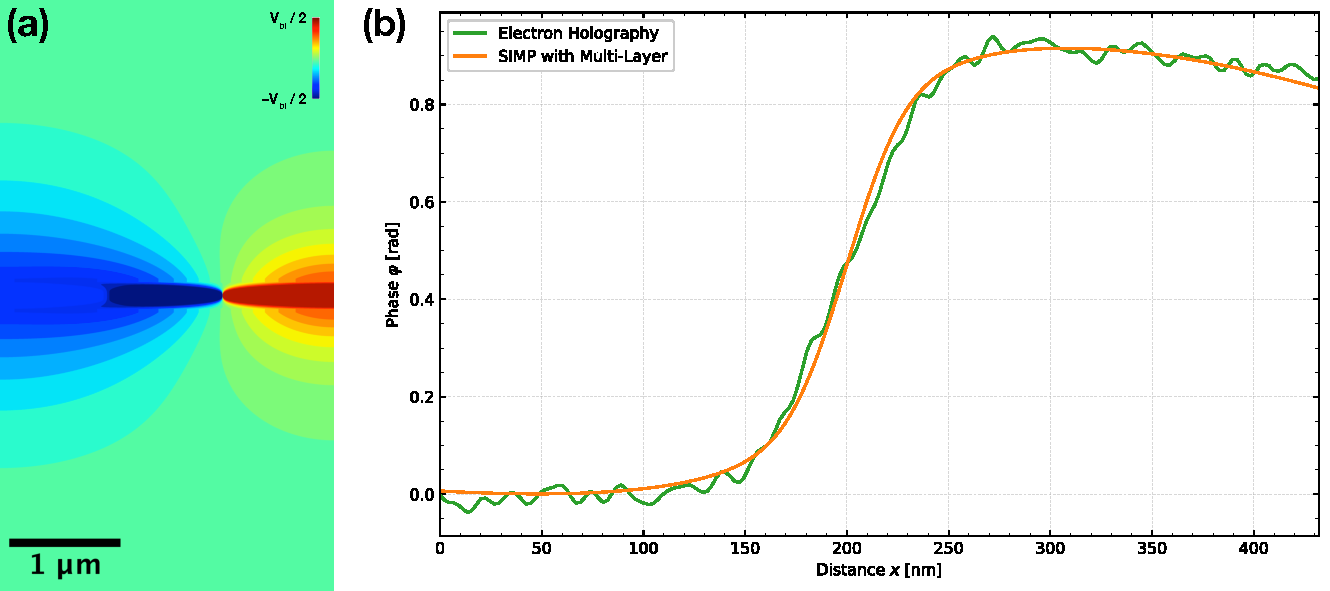
\includegraphics[width=\textwidth]{Figures/Results/pn-Junction/Simulations/ppn-junction-SIMP-multilayer-EH-comparison.pdf}
	\caption{Comparison between the multi-layer framework for \emph{SIMP} and off-axis EH with for the $p$-$p^+$-$n^+$-junction with (a) the 2D~electrostatic potential~$\phi_{\mathit{ML}}$ calculated through the above described multi-layer model and parameters and (b) the phases $\varphi$ obtained through a projection of $\phi$ in propagation direction.}
	\label{fig:ppn-junction-SIMP-multilayer-EH-comparison}
\end{figure}
By comparing the phases $\varphi$ obtained through a projection of the 2D~electrostatic potential~$\phi$ in propagation direction, it is apparent that the same multi-layer framework for \emph{SIMP} is still in great agreement with the experimentally acquired holograms (\cref{fig:ppn-junction-SIMP-multilayer-EH-comparison}b). This is particularly evident when compared to the phases obtained from the \emph{nextnano} simulations, which exhibit large deviations compared to the experimentally acquired holograms (\cref{fig:pn-junction-FEM-EH-linescan-comparison}c). Furthermore, by applying a spatial filter (i.\,e.\ 1D~Gaussian filter) which is equivalent to the mask radius chosen when reconstructing the experimentally acquired electron waves, the phase $\varphi\left(x\right)$ obtained from \emph{SIMP} is in excellent agreement with the experimentally acquired holograms (\cref{fig:ppn-junction-SIMP-multilayer-EH-comparison}b). Additionally, the $p$-$p^+$-junction has no significant influence on the projected electrostatic potential of the $p^+$-$n^+$-junction.

Similar to \cref{ssec:capacitor-SIMP-tomography-comparison}, both the experimentally acquired holograms and the multi-layer \emph{SIMP} framework are tomographically reconstructed and compared for an externally applied bias of $U_{\mathit{ext}} = \SI{2.0}{\volt}$ (\cref{fig:ppn-junction-SIMP-EH-tomography-comparison}). Here, experimentally acquired holograms of the unbiased specimen (i.\,e.\ $U_{\mathit{ext}} = \SI{0}{\volt}$) are used for normalization during the numerical reconstruction process, therefore removing unwanted phase modulations (e.\,g.\ surface charging) and yielding only the change caused by the externally applied bias \cite{Wagner2019}.
\begin{figure}[H]
	\centering
	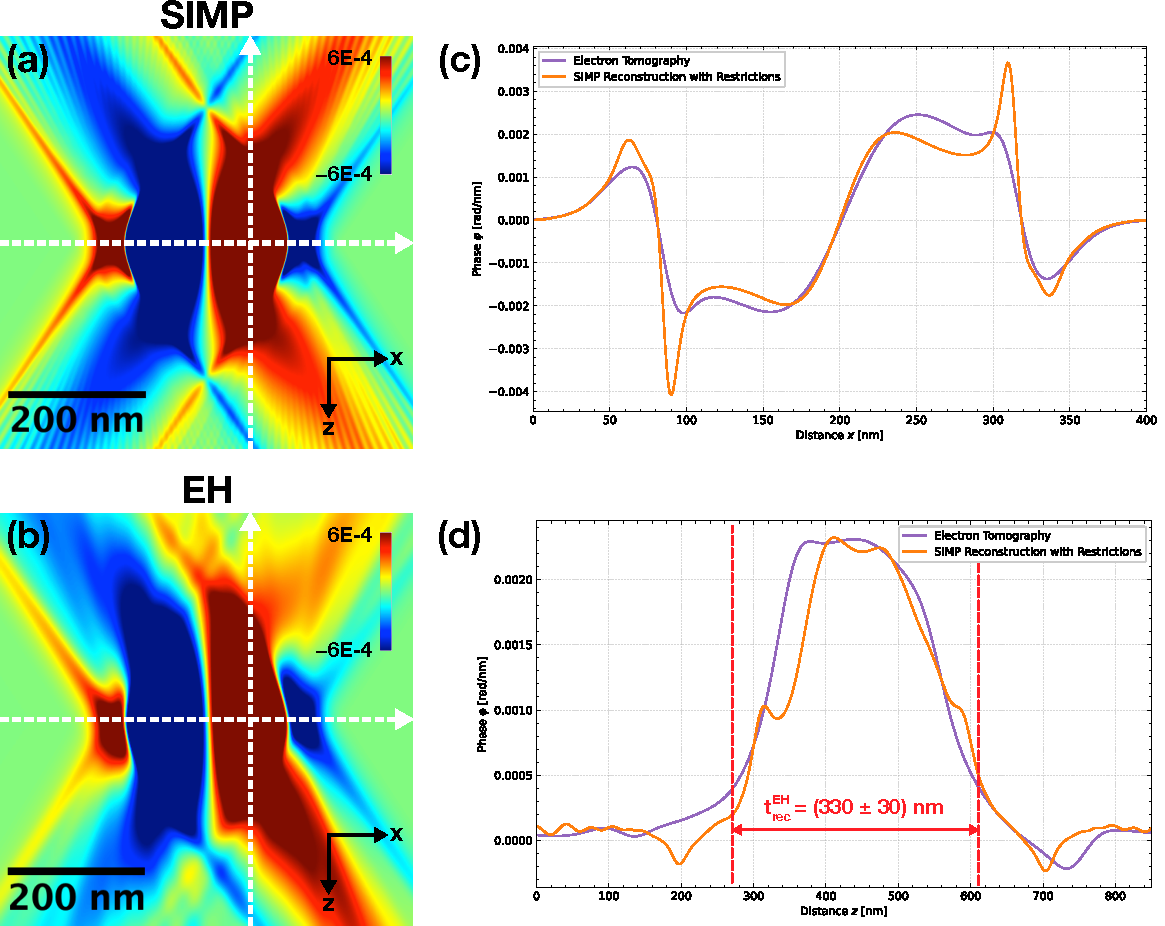
\includegraphics[width=\textwidth]{Figures/Results/pn-Junction/Tomography/ppn-junction-SIMP-EH-tomography-comparison.pdf}
	\caption{Tomographic reconstruction of the $p$-$p^+$-$n^+$-junction with (a) the 2D~back-projected phase $\varphi_{\mathit{rec}}^{\mathit{rest}}$ obtained from the multi-layer \emph{SIMP} framework, (b) the 2D~back-projected phase $\varphi_{\mathit{rec}}^{\mathit{EH}}$ obtained from the experimentally acquired holograms, (c) the line profiles $\varphi\left(x\right)$ across the center of the specimen and (d) the line profiles $\varphi\left(z\right)$ across the $n^+$-region for an externally applied bias of $U_{\mathit{ext}} = \SI{2.0}{\volt}$. For both 2D~back-projected phases, a 2D~Gaussian Blur of $\sigma_G = 4.0$ is applied.}
	\label{fig:ppn-junction-SIMP-EH-tomography-comparison}
\end{figure}
Considering the lines profiles $\varphi\left(z\right)$ (indicated by the white dashed lines in \cref{fig:ppn-junction-SIMP-EH-tomography-comparison}a and b), it is observed that both specimen thicknesses obtained from the multi-layer \emph{SIMP} framework and the experimentally acquired holograms are determined to be $t_{\mathit{rec}}^{\mathit{rest}} = t_{\mathit{rec}}^{\mathit{EH}} = \SI{330 \pm 30}{\nm}$, where both lines profiles are in excellent agreement (\cref{fig:ppn-junction-SIMP-EH-tomography-comparison}d). Despite the strongly restricted angular range of the tomographic tilt series, resulting in a limited spatial resolution in $z$-direction, a considerable reduction in the width of the potential jump located at a central region of specimen (far from the specimen surfaces) is observed in comparison with the classical reconstructed phase (\cref{fig:ppn-junction-SIMP-EH-tomography-comparison}c).

These results further corroborate the validity of the multi-layer framework for \emph{SIMP}, where the bulk core region only contributes a small part to the overall phase and the preparation damage layer caused by the FIB extends deep into the specimen. Furthermore, the multi-layer system determined through \emph{SIMP} is in excellent agreement with the specimen thickness previously obtained through the comparison between off-axis EH and CBED.

The deviations observed towards the edges of the specimen between the experimentally acquired holograms and the multi-layer framework for \emph{SIMP} for the line profiles $\varphi\left(x\right)$ (indicated by the white dashed lines in \cref{fig:ppn-junction-SIMP-EH-tomography-comparison}a and b) can again be attributed to reconstructing artifacts in the FBP. Additionally, the slight asymmetry between the $p^+$-region and $n^+$-region of the experimentally acquired holograms can potentially be attributed, among other things, to a non-zero pre-tilt of the specimen inside the holder, electron beam induced charging of the specimen surface (which is different for the $p^+$-region and $n^+$-region) or the built-up of a surface current when applying an external bias voltage to the specimen (i.\,e.\ shunt resistance).

Similar to the experimentally acquired holograms, the phases $\varphi$ are calculated through the projection of the 2D~electrostatic potential $\phi_{\mathit{ML}}$ obtained from \emph{SIMP} for every tilt angle $\alpha \in \left\{\SI{-34}{\degree}, \SI{-32}{\degree}, \dots , \SI{+32}{\degree}, \SI{+34}{\degree}\right\}$, where a cutout of similar size to the field of view is centered around the depletion region, and modulated through the subtraction of a linear fit, ranging from 10\% to 20\% and extrapolated to the entire field of view, from all values (\cref{ssec:FEM-simulated-potential-and-phase}).

To ensure comparability between \emph{SIMP} and the experimentally measured holograms, the phases for no externally applied bias (i.\,e.\ $U_{\mathit{ext}} = \SI{0}{\volt}$) must be subtracted for the multi-layer framework, as was the case for the experimentally measured $p$-$p^+$-$n^+$-junction. Due to the abnormal switching behavior of the specimen, which is in part caused by the built-up of an Schottky barrier, the increase in the phase jump $\Delta \varphi\left(x\right)$ is not given by \cref{eq:pn-junction-potential}, which would predict a phase jump of $\Delta \varphi\left(x\right) \approx \SI{3.1}{\volt}$, but rather by the considerably smaller change observed in \cref{ssec:experimental-results-ppn-junction-off-axis-EH} (\cref{fig:pn-junction-off-axis-EH-phase-jump}b). After subtracting the phases for no externally applied bias, a spatial filter (i.\,e.\ 1D~Gaussian filter) equivalent to the mask radius chosen when reconstructing the experimentally acquired electron waves is applied.

\emph{SIMP} therefore allows for the approximation of the electrostatic potential distribution in electrically biased complex real-world specimens, especially with regards to the propagation direction of the electron beam, through a limited set of parameters obtained by comparison with only one reconstructed phase.

\chapter{Conclusion and Outlook} \label{chap:Conclusion}
The overarching aim of this thesis was to investigate the influence of surface effects of electrically biased semiconductor nanostructures and their stray fields on measuring electrostatic potentials by means of off-axis electron holography. Therefore, both a combined approach, comparing established simulation methods and electron holographic measurements, was pursued and a completely new model for the approximation of complex potential distributions, which was verified by tomographic investigations, was developed.

In \cref{chap:experimental-methods}, the used experimental methods are presented. For this purpose, special automation routines were developed, which are divided into the measurement of the specimens as well as the reconstruction and post-processing of the measurement data, consequently significantly cutting down on measurement time, reducing the required time (excluding TEM alignment) from a full work day to around 30~minutes or less. Based on this automation routine, the comparison between electron holography and the simulations obtained from the different software packages was deepened in \cref{chap:experimental-results}. Here, it was shown that for both TEM-specimens the stray field extends several $\si{\um}$ deep into the vacuum region above and below the TEM-specimen. Additionally, it was revealed that the contribution of the TEM-specimen to the overall phase modulation is limited compared to the stray field (approximately 8\% for the coplanar capacitor and approximately 12\% for the $p$-$p^+$-$n^+$-junction). An excellent agreement between simulation and experimental results was observed for the coplanar capacitor, especially with respect to the expected linear proportionality between externally applied bias voltage and normalized phase slope. For the semiconductor nanostructure, in contrast, strong discrepancies between simulated and measured phases were observed, which are particularly reflected in a strong broadening of the depletion region as well as in a significantly reduced phase jump (both deviations in the range of one order of magnitude). According to the results, these deviations cannot be attributed to the influence of the stray field or the screening layer (even an extended Debye length of $\lambda_D = \SI{18 \pm 5}{\nm}$ has only a negligible influence on the overall phase modulation), but, according to literature \cite{Twitchett-Harrison2007}, originate from preparation-related Ga-ion implantation. This cannot be reproduced with conventional simulation approaches (classical electrostatic approaches require extensive knowledge about the charge carrier distribution and boundary conditions, rarely known for complex TEM-specimens), which makes a new model for the approximation of such potential distributions of real-world semiconductor nanostructures inevitable.

\Cref{chap:SIMP}, which is the core of this thesis, deals with the introduction, systematic characterization as well as the application of such a model to real-world semiconductor nanostructures, verifying its robustness by means of tomographic investigations. The model provides a simple and intuitive approach for modeling complex potential distributions, where a convolution of a initial potential distribution with a (normalized) propagation distance dependent 1D~Gaussian kernel is utilized. Hereby it is able to approximate the potential distribution of the stray field outside the TEM-specimen as well as any distributions inside the TEM-specimen (e.\,g.\ due to preparation-related artifacts) that may arise, requiring minimal knowledge of the TEM-specimen besides an initial electrostatic potential distribution. From a numerical standpoint, the presented model allows for a linear scaling with available computational power through a parallelization of the independent calculations of all intermediate results, which leads to a significant reduction of computation time and required memory (i.\,e.\ seconds instead of days and a few~GBs instead of hundreds of~GBs, respectively). Utilizing the coplanar capacitor as a well known reference specimen, the model was thoroughly tested and characterized for different geometric layouts (i.\,e.\ varying distance between the capacitor plates), resulting in a maximum deviation of $\Delta \phi_{\mathit{max}} = \SI{0.1}{\volt}$ (limited only to an area close to the contacts, where the theoretical approximations made in the model are no longer valid) in a direct comparison with finite element simulations. An excellent agreement between the model and experimental results was shown in particular with tomographic investigations, where the tilt series was limited to an angular range of $\alpha = \pm \SI{34}{\degree}$ in $\SI{2}{\degree}$ increments. Here, the spacing of the capacitor plates was accurately determined to $d_{\mathit{rec}}^{\mathit{rest}} = \SI{480 \pm 20}{\nm}$ and the thickness of the specimen to be $t_{\mathit{rec}}^{\mathit{rest}} = \SI{500 \pm 50}{\nm}$

For a $p$-$p^+$-$n^+$-junction, the self-developed model was extended to a multi-layer framework, consisting of a bulk core, preparation damage and surface layer region (where the preparation damage layer correlates to a region with a FIB-induced changing electrostatic potential distribution in electron beam direction). Through the comparison of CBED and EH measurements, the thickness of the surface was determined to be $t_{\mathit{SL}} = \SI{30 \pm 5}{\nm}$. The bulk core thickness of $t_{\mathit{BC}} = \SI{10}{\nm}$, determined through a comparison with a single reconstructed phase, yields a preparation damage depth of $t_{\mathit{PD}} = \SI{110}{\nm}$. By using these parameters for the approximation of the electrostatic potential distribution, a tomographic comparison (analog to the coplanar capacitor) yielded an excellent agreement between the self-developed model and experimental results. In detail, the specimen thicknesses determined from both methods match within the limits of their measurement uncertainty with $t_{\mathit{rec}}^{\mathit{rest}} = t_{\mathit{rec}}^{\mathit{EH}} = \SI{330 \pm 30}{\nm}$. Moreover, despite the limited resolution in $z$-direction (i.\,e.\ strongly restricted angular range), a significantly reduced width of the potential jump in a central region of the specimen (far from the specimen surfaces) is observed compared to the classical reconstructed phase. The excellent agreement of both tomographic reconstructions validates the self-developed model, where all necessary parameters were obtained from the comparison with only one reconstructed phase. A sufficiently good knowledge of the potential distribution of real-world TEM-specimens (in particular in electron beam direction) can consequently be obtained on the basis of this model with significantly reduced measurement and computational effort.

These findings show that the first major hurdle towards the quantitative investigation of real-world semiconductor nanostructures has been overcome. However, there are still some small hurdles on the way to the finish line. On the one hand, biased TEM-specimens show surface currents and charging effects, which raise the question to what extent a variation of the surface layer in the self-developed model is necessary. On the other hand, a systematic investigation of the influences of FIB parameters, such as the beam current or the acceleration voltage during specimen preparation, is required in order to match them with the adjustable model parameters (e.\,g.\ implantation depth $t_{\mathit{PD}}$). These systematic investigations would go far beyond the scope of this thesis, but provide sufficient basis for further in-depth studies of this highly interesting topic. Nevertheless, this thesis has provided a completely new set of methodological tools for investigating the influence of surface effects of electrically biased semiconductor nanostructures on EH investigations.


\printbibliography[heading=bibintoc]
\appendix
\chapter{Convergent-Beam Electron Diffraction} \label{chap:appendix-CBED}
If the specimen is illuminated by a parallel plane electron wave, electron diffraction, which is caused by electron scattering due to interaction with the atoms, occurs and the intensity in the far-field is given by:
\begin{equation}
  I\left(\vb{k}\right) = \lvert\mathcal{F}\left\{\psi_{\mathit{obj}}\left(\vb{k}\right)\right\}\rvert^2 \quad ; \quad \vb{k} = \frac{\theta}{\lambda},
\end{equation}
where $\psi_{\mathit{obj}}$ is the object wave modulated by the specimen, $\vb{k}$ the scattering vector in the detector plane and $\theta$ the scattering angle \cite{Hawkes2019,Williams2009}.

By choosing the (diffraction-limited) probe such that it is significantly larger than the electron source at the specimen, the probe described by the convergent electron beam can be considered as coherent \cite{Hawkes2019,Williams2009}. If the investigated specimen is crystalline, it therefore diffracts the electrons into discrete Bragg beams, which are broadened into discs when using the electron microscope in STEM~mode \cite{Hawkes2019,Williams2009}.
\newpage
Consequently, convergent-beam electron diffraction (CBED) allows for the measurement of the crystalline part of a specimen's thickness $t_{\mathit{CBED}}$ through a comparison with corresponding simulations (\cref{fig:CBED-comparison-simulation-thickness}).\footnote{All measurement data, simulations, analyses and plots were graciously provided by Dr.~Ines Häuser from the Humboldt University of Berlin.}
\begin{figure}[H]
  \centering
  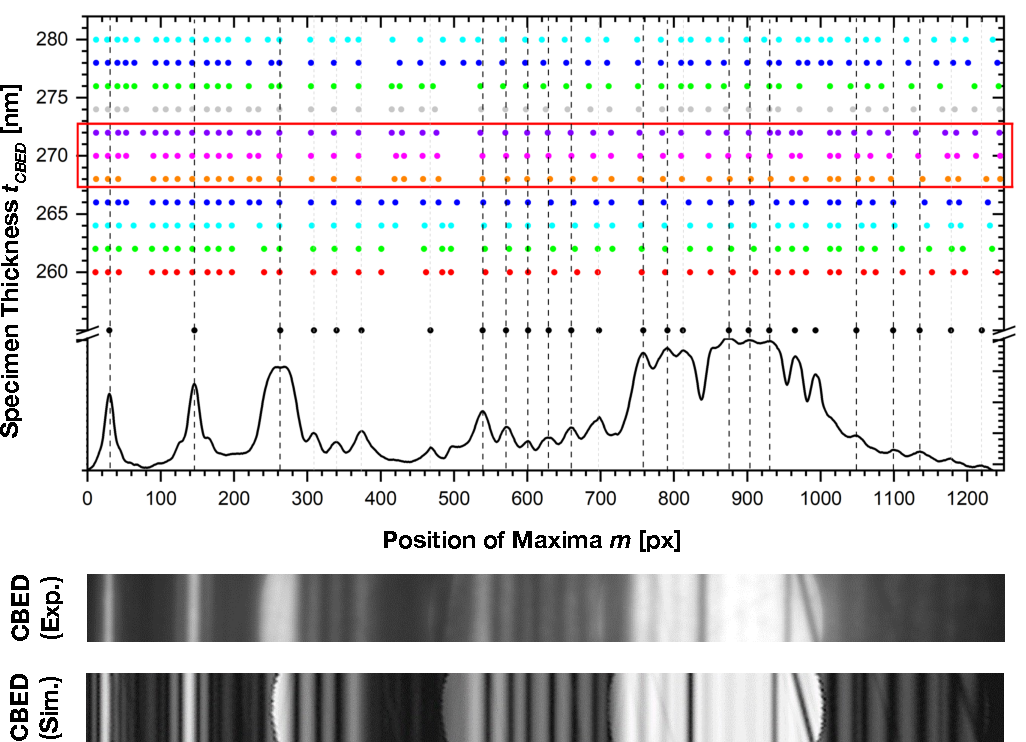
\includegraphics[width=\textwidth]{Figures/Specimen/pn-Junction/CBED-comparion-simulation-thickness.pdf}
  \caption{Determination of the specimen thickness $t_{\mathit{CBED}}$ from the comparison between CBED simulations and the experimental measurement. The thickness can be obtained by finding the corresponding simulation where the positions of the maxima $m$ of the HOLZ lines are in best agreement with the experimentally obtained diffraction pattern (indicated by the red rectangle).}
  \label{fig:CBED-comparison-simulation-thickness}
\end{figure}
For this purpose, the specimen is simulated with different thicknesses using the \emph{JEMS} software package \cite{JEMS}. By matching the position of the maxima $m$ of the higher-order Laue zones (HOLZ) lines, the crystalline part of the specimen thickness is determined to be $t_{\mathit{CBED}} = \SI{270 \pm 2}{\nm}$ (\cref{fig:CBED-comparison-simulation-thickness}, indicated by the red rectangle).

\chapter{Specimen Thickness Through Off-Axis Electron Holography} \label{chap:appendix-specimen-thickness-off-axis-EH}
Contrary to CBED (\cref{chap:appendix-CBED}), the phase shift measured in off-axis EH is dependent on the whole specimen thickness $t_{\mathit{EH}}$ and can therefore be directly calculated through the measured phase shift (\cref{fig:pn-junction-thickness-off-axis-EH}):
\begin{equation}
  \label{eq:specimen-thickness-phase-shift}
  t_{\mathit{EH}} = \frac{\varphi_{\mathit{obj}}\left(\vb{r}\right)}{\sigma \phi_{\mathit{MIP}}\left(\vb{r}\right)},
\end{equation}
where $\sigma = \pi / \lambda E$ is an acceleration voltage dependent interaction constant and $\phi_{\mathit{MIP}}\left(\vb{r}\right)$ is the mean inner potential of the specimen \cite{Voelkl1999,Lehmann2002,Lichte2008}.
\begin{figure}[H]
  \centering
  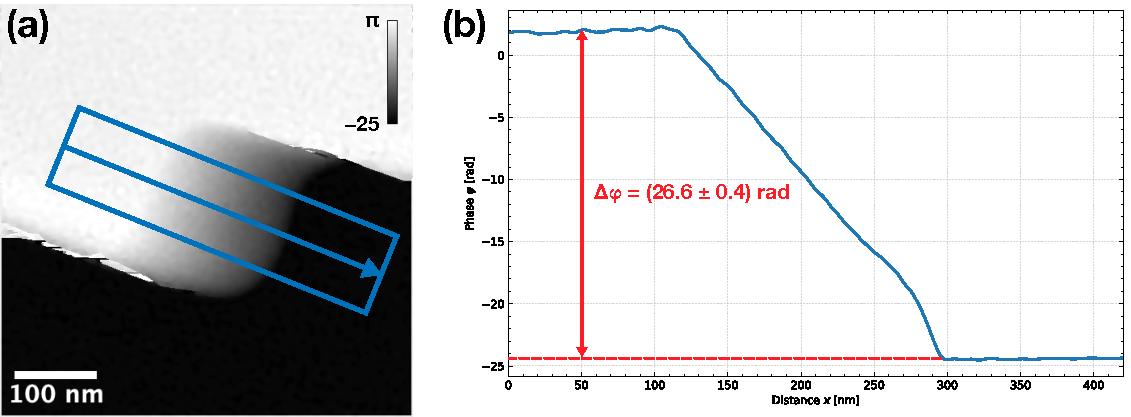
\includegraphics[width=\textwidth]{Figures/Specimen/pn-Junction/off-axis-EH-thickness.pdf}
  \caption{Determination of the specimen thickness $t_{\mathit{EH}}$ from off-axis EH with (a)~the reconstructed unwrapped phase $\varphi$ and (b) its corresponding line profile $\varphi\left(x\right)$. The specimen thickness is determined through the phase jump $\Delta \varphi = \SI{26.6 \pm 0.4}{rad}$ measured at the gradient of the specimen edge.}
  \label{fig:pn-junction-thickness-off-axis-EH}
\end{figure}
Using \cref{eq:specimen-thickness-phase-shift}, the measured phase jump of $\Delta \varphi = \SI{26.6 \pm 0.4}{rad}$ (where the measurement uncertainty is given by the standard deviation in the noise of the phase~$\varphi$), an interaction constant of $\sigma = \SI{6.53}{rad \per \volt \um}$ \cite{Beleggia2014} and a mean inner potential of $\phi_{\mathit{MIP}}\left(\vb{r}\right) = \SI{12.57}{\volt}$ for Si \cite{Kruse2006}, the specimen thickness is determined to be $t_{\mathit{EH}} = \SI{325 \pm 5}{\nm}$.

\chapter*{Acknowledgments}
The completion of this thesis could not have been possible without the help of my first examiner Prof.~Dr.~Michael Lehmann, whom I would like to sincerely thank for all the great scientific discussions we had as well as the opportunity to use his excellent laboratory.

My deepest gratitude goes to my supervisor Dr.~Tolga Wagner, who has accompanied me, both personally and scientifically, on this journey from the very beginning.

I would like to thank Dr.~Andrei Schliwa for assuming the role as second examiner, for his help with acquiring a license for the \emph{nextnano} software package and for all the productive scientific discussions we had.

I am sincerely grateful to my friend and colleague Robert Fuchs, without whose valuable discussions the mathematical foundation of \emph{SIMP} would never have come about.

I owe a debt of gratitude to my esteemed colleague Dr.~Ines Häusler from the Humboldt University of Berlin for providing me with the CBED measurement data and analysis of the $p$-$p^+$-$n^+$-junction.

Furthermore, I would like to thank my entire work group, especially Elke Wandke, for the warm reception I received from the very beginning.

I am thankful to the members of the ZELMI of the Technische Universität Berlin, especially Dr.~Christian Günther and Dr.~Dirk Berger, for providing me with the specimens and a pleasant work environment in the laboratory.

I also thank Henrik Wähnert, Jan Simke and Dr.~Nina Owschimikow for the sometimes much needed distraction and all the great conversations we had.

At last, my deepest gratitude goes to my parents Dürdane and Ali Çelik, who have given me the opportunity to pursue this degree.

\end{document}
